%%% Copyright (C) 2017 Vincent Goulet
%%%
%%% Ce fichier et tous les fichiers .tex ou .Rnw dont la racine est
%%% mentionnée dans les commandes \include ci-dessous font partie du
%%% projet «Programmer avec R»
%%% http://github.com/vigou3/programmer-avec-r
%%%
%%% Cette création est mise à disposition selon le contrat
%%% Attribution-Partage dans les mêmes conditions 4.0
%%% International de Creative Commons.
%%% http://creativecommons.org/licenses/by-sa/4.0/

\documentclass[letterpaper,11pt,x11names,english,french]{memoir}
  \usepackage{natbib,url}
  \usepackage{babel}
  \usepackage[autolanguage]{numprint}
  \usepackage{amsmath,amsthm}
  \usepackage[noae]{Sweave}
  \usepackage{framed}                  % env. snugshade*, oframed
  \usepackage{paralist}
  \usepackage[shortlabels]{enumitem}
  \usepackage[absolute]{textpos}       % éléments des pages de titre
  \usepackage{graphicx}
  \usepackage{manfnt}                  % \mantriangleright (puce)
  \usepackage{metalogo}                % \XeLaTeX logo
  \usepackage{applekeys}               % touches Mac
  \usepackage{fontawesome}             % icônes \fa*
  \usepackage{answers}                 % exercices et solutions
  \usepackage{listings}                % code informatique
  \usepackage{pgf}                     % transparence pour couverture avant

  %%% =============================
  %%%  Informations de publication
  %%% =============================
  \title{Programmer avec R}
  \author{Vincent Goulet}
  \renewcommand{\year}{2017}
  \renewcommand{\month}{08-1}
  \newcommand{\ISBN}{}
  \newcommand{\ghurl}{https://github.com/vigou3/programmer-avec-r/}

  %%% ===================
  %%%  Style du document
  %%% ===================

  %% Polices de caractères
  \usepackage{fontspec}
  \usepackage{unicode-math}
  \defaultfontfeatures{Scale=0.92}
  \setmainfont[Ligatures=TeX,Numbers=OldStyle]{Lucida Bright OT}
  \setmathfont{Lucida Bright Math OT}
  \setmonofont{Lucida Grande Mono DK}
  \setsansfont[Scale=1.0,Numbers=OldStyle]{Myriad Pro}
  \newfontfamily\fullcaps[Letters=Uppercase,Numbers=Uppercase]{Myriad Pro}
  \usepackage[babel=true]{microtype}
  \usepackage{icomma}

  %% Couleurs
  \usepackage{xcolor}
  \definecolor{comments}{rgb}{0.7,0,0}      % commentaires
  \definecolor{link}{rgb}{0,0.4,0.6}        % liens internes
  \definecolor{url}{rgb}{0.6,0,0}           % liens externes
  \definecolor{citation}{rgb}{0,0.5,0}      % citations
  \definecolor{codebg}{named}{LightYellow1} % fond code R
  \definecolor{prob}{named}{orange}         % encadrés «problème»
  \definecolor{rouge}{rgb}{0.85,0,0.07} % rouge bandeau identitaire
  \definecolor{or}{rgb}{1,0.8,0}        % or bandeau identitaire

  %% Hyperliens
  \usepackage{hyperref}
  \hypersetup{%
    pdfauthor = \theauthor,
    pdftitle = \thetitle,
    colorlinks = {true},
    linktocpage = {true},
    urlcolor = {url},
    linkcolor = {link},
    citecolor = {citation},
    pdfpagemode = {UseOutlines},
    pdfstartview = {Fit},
    bookmarksopen = {true},
    bookmarksnumbered = {true},
    bookmarksdepth = {subsubsection}}
  \setlength{\XeTeXLinkMargin}{1pt}

  %% Étiquettes de \autoref (redéfinitions compatibles avec babel).
  %% Attention! Les % à la fin des lignes sont importants sinon des
  %% blancs apparaissent dès que la commande \selectlanguage est
  %% utilisée... comme dans la bibliographie, par exemple.
  \addto\extrasfrench{%
    \def\appendixautorefname{annexe}%
    \def\figureautorefname{figure}%
    \def\exempleautorefname{exemple}%
    \def\exerciceautorefname{exercice}%
    \def\subfigureautorefname{figure}%
    \def\subsectionautorefname{section}%
    \def\subtableautorefname{tableau}%
    \def\tableautorefname{tableau}%
  }

  %% Table des matières (inspirée de classicthesis.sty)
  \renewcommand{\cftchapterleader}{\hspace{1.5em}}
  \renewcommand{\cftchapterafterpnum}{\cftparfillskip}
  \renewcommand{\cftsectionleader}{\hspace{1.5em}}
  \renewcommand{\cftsectionafterpnum}{\cftparfillskip}

  %% Titres des chapitres
  \chapterstyle{hangnum}
  \renewcommand{\chaptitlefont}{\normalfont\Huge\sffamily\bfseries\raggedright}

  %% Marges, entêtes et pieds de page
  \setlength{\marginparsep}{7mm}
  \setlength{\marginparwidth}{13mm}
  \setlength{\headwidth}{\textwidth}
  \addtolength{\headwidth}{\marginparsep}
  \addtolength{\headwidth}{\marginparwidth}

  %% Titres des sections et sous-sections
  \setsecheadstyle{\normalfont\Large\sffamily\bfseries\raggedright}
  \setsubsecheadstyle{\normalfont\large\sffamily\bfseries\raggedright}
  \maxsecnumdepth{subsection}
  \setsecnumdepth{subsection}

  %% Listes. Paramétrage avec enumitem.
  \setlist[enumerate]{leftmargin=*,align=left}
  \setlist[enumerate,2]{label=\alph*),labelsep=*,leftmargin=1.5em}
  \setlist[enumerate,3]{label=\roman*),labelsep=*,leftmargin=1.5em,align=right}
  \setlist[itemize]{leftmargin=*,align=left}

  %% Options de babel
  \frenchbsetup{CompactItemize=false,%
    ThinSpaceInFrenchNumbers=true,
    ItemLabeli=\mantriangleright,
    ItemLabelii=\textendash,
    og=«, fg=»}
  \addto\captionsfrench{\def\figurename{{\scshape Fig.}}}
  \addto\captionsfrench{\def\tablename{{\scshape Tab.}}}

  %%% =========================
  %%%  Sections de code source
  %%% =========================
  \lstloadlanguages{R}
  \lstdefinelanguage{Renhanced}[]{R}{%
    morekeywords={colMeans,colSums,head,is.na,is.null,mapply,ms,na.rm,%
      nlmin,replicate,row.names,rowMeans,rowSums,sys.time,system.time,%
      tail,which.max,which.min},
    deletekeywords={c,start},
    alsoletter={.\%},%
    alsoother={:_\$}}
  \lstset{language=Renhanced,
    extendedchars=true,
    basicstyle=\small\ttfamily\NoAutoSpacing,
    commentstyle=\color{comments}\slshape,
    keywordstyle=\mdseries,
    showstringspaces=false,
    index=[1][keywords],
    indexstyle=\indexfonction}

  %%% =========================
  %%%  Nouveaux environnements
  %%% =========================

  %% Environnements d'exemples et al.
  \theoremstyle{remark}
  \newtheorem*{rem}{Remarque}
  \newtheorem*{rems}{Remarques}

  %% Redéfinition de l'environnement titled-frame de framed.sty avec
  %% deux modifications: épaisseur des filets réduite de 2pt à 1pt;
  %% "(suite)" plutôt que "(cont)" dans la barre de titre
  %% lorsque l'encadré se poursuit après un saut de page.
  \renewenvironment{titled-frame}[1]{%
    \def\FrameCommand{\fboxsep8pt\fboxrule1pt
      \TitleBarFrame{\textbf{#1}}}%
    \def\FirstFrameCommand{\fboxsep8pt\fboxrule1pt
      \TitleBarFrame[$\blacktriangleright$]{\textbf{#1}}}%
    \def\MidFrameCommand{\fboxsep8pt\fboxrule1pt
      \TitleBarFrame[$\blacktriangleright$]{\textbf{#1\ (suite)}}}%
    \def\LastFrameCommand{\fboxsep8pt\fboxrule1pt
      \TitleBarFrame{\textbf{#1\ (suite)}}}%
    \MakeFramed{\advance\hsize-16pt \FrameRestore}}%
  {\endMakeFramed}

  %% Encadré générique avec titre basé sur titled-frame, ci-dessus.
  %% Sert pour les listes d'objectifs et les encadrés reliés aux
  %% problèmes (mises en situation) dans les chapitres. Arguments:
  %% couleur du cadre (optionnel; noir par défaut) et titre de la
  %% boîte (obligatoire).
  \newenvironment{emphbox}[2][black]{%
    \colorlet{TFFrameColor}{#1}%
    \colorlet{TFTitleColor}{white}%
    \begin{titled-frame}{\sffamily #2}%
      \setlength{\parindent}{0pt}}%
    {\end{titled-frame}}

  %% Liste d'objectifs au début des chapitres
  \newenvironment{objectifs}{%
    \begin{emphbox}{\rule[-7pt]{0pt}{20pt} Objectifs du chapitre}
      \begin{itemize}[nosep]
        \small\sffamily}%
      {\end{itemize}\end{emphbox}}

  %% Problèmes (mises en situation) des chapitres: énoncé au début du
  %% chapitre; astuces en cours de chapitre; solution à la fin
  %% du chapitre.
  \newenvironment{prob-enonce}{%
    \begin{emphbox}[prob]{{\normalfont\faCogs}\; Énoncé du problème}}%
    {\end{emphbox}}
  \newenvironment{prob-astuce}{%
    \begin{emphbox}[prob]{{\normalfont\faBolt}\; Astuce}}%
    {\end{emphbox}}
  \newenvironment{prob-solution}{%
    \begin{emphbox}[prob]{{\normalfont\faLightbulbO}\; Solution du problème}}%
    {\end{emphbox}}

  %% Environnements de Sweave. Les environnements Sinput et Soutput
  %% utilisent Verbatim (de fancyvrb). On les réinitialise pour
  %% enlever la configuration par défaut de Sweave, puis on réduit
  %% l'écart entre les blocs Sinput et Soutput. L'environnement Schunk
  %% est complètement redéfini à partir de snugshade* (de framed) pour
  %% insérer un fond de couleur derrière les blocs de code source.
  \DefineVerbatimEnvironment{Sinput}{Verbatim}{}
  \DefineVerbatimEnvironment{Soutput}{Verbatim}{}
  \fvset{listparameters={\setlength{\topsep}{0pt}}}
  \renewenvironment{Schunk}{%
    \setlength{\topsep}{0pt}
    \colorlet{shadecolor}{codebg}
    \begin{snugshade*}}%
    {\end{snugshade*}}

  %% Exercices et réponses
  \Newassociation{sol}{solution}{solutions}
  \newcounter{exercice}[chapter]
  \renewcommand{\theexercice}{\thechapter.\arabic{exercice}}
  \newenvironment{exercice}[1][]{%
    \begin{list}{}{%
        \refstepcounter{exercice}
        \ifthenelse{\equal{#1}{nosol}}{%
          \renewcommand{\makelabel}{\bfseries\theexercice}}{%
          \hypertarget{ex:\theexercice}{}
          \Writetofile{solutions}{\protect\hypertarget{sol:\theexercice}{}}
          \renewcommand{\makelabel}{%
            \bfseries\protect\hyperlink{sol:\theexercice}{\theexercice}}}
        \settowidth{\labelwidth}{\bfseries\theexercice}
        \setlength{\leftmargin}{\labelwidth}
        \addtolength{\leftmargin}{\labelsep}
        \setlist[enumerate,1]{label=\alph*),labelsep=*,leftmargin=1.5em}
        \setlist[enumerate,2]{label=\roman*),labelsep=0.5em,align=right}}
      \item}%
      {\end{list}}
  \renewenvironment{solution}[1]{%
    \begin{list}{}{%
        \renewcommand{\makelabel}{%
          \bfseries\protect\hyperlink{ex:#1}{#1}}
        \settowidth{\labelwidth}{\bfseries #1}
        \setlength{\leftmargin}{\labelwidth}
        \addtolength{\leftmargin}{\labelsep}
        \setlist[enumerate,1]{label=\alph*),labelsep=*,leftmargin=1.5em}
        \setlist[enumerate,2]{label=\roman*),labelsep=0.5em,align=right}}
      \item}
    {\end{list}}

  %% Encadré générique pour les remarques importantes et autres
  %% comportant une icône sur la gauche. Argument: symbole à
  %% placer sur la gauche (obligatoire).
  \newenvironment{infobox}[1]{%
    \setlength{\FrameRule}{1pt}
    \begin{framed}%
      \noindent
      \begin{minipage}{0.1\linewidth}
        \raisebox{-1.5em}[0em][0em]{\HUGE#1}
      \end{minipage}
      \begin{minipage}[t]{0.88\linewidth}}%
      {\end{minipage}\end{framed}}

  %% Remarques importantes
  \newenvironment{important}{%
    \begin{infobox}{\faExclamationCircle}}%
    {\end{infobox}}

  %% Informations
  \newenvironment{information}{%
    \begin{infobox}{\faInfoCircle}}%
    {\end{infobox}}

  %% Remarques spécifiques OS X
  \newenvironment{osx}{%
    \begin{infobox}{\faApple}}%
    {\end{infobox}}

  %% Listes de commandes
  \newenvironment{ttscript}[1]{%
    \begin{list}{}{%
        \setlength{\labelsep}{1.5ex}
        \settowidth{\labelwidth}{\fbox{\code{#1}}}
        \setlength{\leftmargin}{\labelwidth}
        \addtolength{\leftmargin}{\labelsep}
        \setlength{\parsep}{0.5ex plus0.2ex minus0.2ex}
        \setlength{\itemsep}{0.3ex}
        \renewcommand{\makelabel}[1]{\fbox{\vphantom{|}##1}\hfill}}}
    {\end{list}}

  %%% Chapitre Opérateurs: l'espacement entre les expressions R et
  %%% leur sortie est réduit pour les exemples de fonctions.
  \newlength{\compactsep} \setlength{\compactsep}{-0.5ex}
  \newlength{\normalsep}  \setlength{\normalsep}{\topsep}

  %%% Listes de structures de contrôle
  \newenvironment{struclist}{%
    \begin{description}[style=nextline,font=\mdseries\ttfamily]}
    {\end{description}}

  %%% =====================
  %%%  Nouvelles commandes
  %%% =====================

  %% Noms de fonctions, code, etc.
  \newcommand{\code}[1]{\texttt{#1}}
  \newcommand{\pkg}[1]{\textbf{#1}}

  %% Indications de capsule vidéo
  \newcommand{\capsule}[2]{\href{#1}{#2}\marginpar{%
      \href{#1}{\raisebox{-0.5em}[0em][0em]{\HUGE\faYoutubePlay}}}}

  %% Hyperlien avec symbole de lien externe juste après
  \newcommand{\link}[2]{\href{#1}{#2~\raisebox{-0.2ex}{\faExternalLink}}}

  %% Lien vers GitHub dans la page de notices
  \newcommand{\viewsource}[1]{%
    \href{#1}{%
      Voir sur GitHub \raisebox{-1pt}{\footnotesize\faGithub}}}

  %% Raccourcis usuels vg
  \newcommand{\pt}{{\scriptscriptstyle \Sigma}}
  \newcommand{\mat}[1]{\mathbf{#1}}
  \newcommand{\var}[1]{\operatorname{Var} [ #1 ]}

  %%% =======
  %%%  Index
  %%% =======
  \newcommand{\bfhyperpage}[1]{\textbf{\hyperpage{#1}}}
  \renewcommand{\preindexhook}{%
    Les numéros de page en caractères gras indiquent les pages où les
    concepts sont introduits, définis ou expliqués.\vskip\onelineskip}
  \newcommand{\Index}[1]{\index{#1|bfhyperpage}}
  \newcommand{\indexargument}[1]{\index{#1@\code{#1}}}
  \newcommand{\Indexargument}[1]{\Index{#1@\code{#1}}}
  \newcommand{\indexattribut}[1]{\index{#1@\code{#1} (attribut)}}
  \newcommand{\Indexattribut}[1]{\Index{#1@\code{#1} (attribut)}}
  \newcommand{\indexclasse}[1]{\index{#1@\code{#1} (classe)}}
  \newcommand{\Indexclasse}[1]{\Index{#1@\code{#1} (classe)}}
  \newcommand{\indexfonction}[1]{\index{#1@\code{#1}}}
  \newcommand{\Indexfonction}[1]{\Index{#1@\code{#1}}}
  \newcommand{\indexmode}[1]{\index{#1@\code{#1} (mode)}}
  \newcommand{\Indexmode}[1]{\Index{#1@\code{#1} (mode)}}
  \newcommand{\indexobjet}[1]{\index{#1@\code{#1}}}
  \newcommand{\Indexobjet}[1]{\Index{#1@\code{#1}}}

  \newcommand{\attribut}[1]{\code{#1}\indexattribut{#1}}
  \newcommand{\Attribut}[1]{\code{#1}\Indexattribut{#1}}
  \newcommand{\argument}[1]{\code{#1}\indexargument{#1}}
  \newcommand{\Argument}[1]{\code{#1}\Indexargument{#1}}
  \newcommand{\classe}[1]{\code{#1}\indexclasse{#1}}
  \newcommand{\Classe}[1]{\code{#1}\Indexclasse{#1}}
  \newcommand{\fonction}[1]{\code{#1}\indexfonction{#1}}
  \newcommand{\Fonction}[1]{\code{#1}\Indexfonction{#1}}
  \newcommand{\mode}[1]{\code{#1}\indexmode{#1}}
  \newcommand{\Mode}[1]{\code{#1}\Indexmode{#1}}
  \newcommand{\objet}[1]{\code{#1}\indexobjet{#1}}
  \newcommand{\Objet}[1]{\code{#1}\Indexobjet{#1}}
  \makeindex

  %%% =======
  %%%  Varia
  %%% =======

  %%% Sous-figures
  \newsubfloat{figure}

  %%% Style de la bibliographie
  \bibliographystyle{francais}

  %% Longueurs pour la composition des pages couvertures avant et
  %% arrière.
  \newlength{\banderougewidth} \newlength{\banderougeheight}
  \newlength{\bandeorwidth}    \newlength{\bandeorheight}
  \newlength{\imageheight}
  \newlength{\logoheight}
  \newlength{\gapwidth}

  %% Aide pour la césure
  \hyphenation{%
    con-naî-tre
    con-sole
    cons-tante
    con-tenu
    con-trôle
    nom-bre
    puis-que
  }

  \includeonly{informatique}

\begin{document}

\frontmatter

\pagestyle{empty}

%%%
%%% Page de titre
%%%

\begingroup
\TPGrid{3}{36}
\textblockorigin{0mm}{0mm}
\setlength{\parindent}{0mm}
\setlength{\imageheight}{29\TPVertModule}
\setlength{\banderougewidth}{2\TPHorizModule}
\setlength{\banderougeheight}{\TPVertModule}
\setlength{\bandeorwidth}{\TPHorizModule}
\setlength{\bandeorheight}{\banderougeheight}
\setlength{\logoheight}{2.5\TPVertModule}
\setlength{\gapwidth}{1.5pt}
\addtolength{\bandeorwidth}{-\gapwidth}
\addtolength{\imageheight}{-\gapwidth}

%% bandeau identitaire
\begin{textblock*}{\paperwidth}[0,1](0mm,30\TPVertModule)
  \textcolor{rouge}{\rule{\banderougewidth}{\banderougeheight}}% % bande rouge
  \rule{\gapwidth}{0pt}%                                         % filet
  \textcolor{or}{\rule{\bandeorwidth}{\bandeorheight}}           % bande or
\end{textblock*}

%% logo UL
\begin{textblock*}{\TPHorizModule}(2\TPHorizModule,31\TPVertModule)
  \rule{\gapwidth}{0pt}%                                         % filet
  \includegraphics[height=\logoheight,%
                   keepaspectratio=true]{ul_p}
\end{textblock*}

%% image de fond
\begin{textblock*}{\paperwidth}(0mm,0mm)
  \includegraphics[height=\imageheight,%
                   width=\paperwidth,%
                   trim=446 0 281 0]{}
\end{textblock*}

%% titre
\begin{textblock*}{\paperwidth}(0.3\TPHorizModule,5.5\TPVertModule)
  \color{white} \thetitle
\end{textblock*}

%% auteur
\begin{textblock*}{\paperwidth}(0.3\TPHorizModule,10\TPVertModule)
  \color{white} \theauthor
\end{textblock*}

\null\cleardoublepage

%%%
%%% Page frontispice
%%%

%% titre
\begin{textblock*}{\paperwidth}(0.3\TPHorizModule,5.5\TPVertModule)
  \thetitle
\end{textblock*}

%% auteur
\begin{textblock*}{2\TPHorizModule}(0.3\TPHorizModule,10\TPVertModule)
  \theauthor \\
  \mdseries
  Professeur titulaire \\
  École d'actuariat, Université Laval
\end{textblock*}

%% édition
\begin{textblock*}{1.7\TPHorizModule}(0.3\TPHorizModule,30\TPVertModule)
  \thedate
\end{textblock*}
\endgroup

%%% Local Variables:
%%% mode: latex
%%% TeX-master: "programmer-avec-r"
%%% TeX-engine: xetex
%%% End:

\null\cleardoublepage           % cf. section 2.2 textpos.pdf

\begingroup
\calccentering{\unitlength}
\begin{adjustwidth*}{\unitlength}{-\unitlength}
  \setlength{\parindent}{0pt}
  \setlength{\parskip}{\baselineskip}

  {\textcopyright} 2012 Vincent Goulet \\

  \includegraphics{gfdl}\\%
  Il est permis de copier, distribuer ou modifier ce document selon
  les termes de la \emph{GNU Free Documentation License}, version 1.3
  ou toute version subséquente publiée par la Free Software
  Foundation; avec aucune section inaltérable (\emph{Invariant
    Sections}), aucun texte de couverture avant (\emph{Front-Cover
    Texts}), et aucun texte de couverture arrière (\emph{Back-Cover
    Texts}). Une copie de la licence est incluse à l'annexe
  \ref{fdl}.

  \textbf{Code source} \\
  Le code source {\LaTeX} et R de ce document est disponible dans le
  dépôt Subversion
  \begin{quote}
    \sloppy
    \url{https://svn.fsg.ulaval.ca/svn-pub/vgoulet/documents/intro_r/}
  \end{quote}
  ou en communiquant directement avec l'auteur.

  \textbf{Historique de publication} \\
  \begin{tabbing}
    Avril 2012:\quad    \= Troisième édition \\
    Janvier 2007:       \> Seconde édition \\
    Janvier 2006:       \> Première édition \\
  \end{tabbing}

  ISBN \ISBN \\
  Dépôt légal -- Bibliothèque nationale du Québec, 2012 \\
  Dépôt légal -- Bibliothèque et Archives Canada, 2012

  \textbf{Couverture} \\
  Tornade de catégorie F5 à l'approche de la ville de Elie, Manitoba,
  le 22 juin 2007.

  Crédits photo: Justin1569 via Wikimedia Commons \\
\end{adjustwidth*}
\endgroup

%%% Local Variables:
%%% mode: latex
%%% TeX-master: "introduction_programmation_r"
%%% coding: utf-8
%%% End:

\clearpage

\pagestyle{companion}

\chapter*{Introduction}
\addcontentsline{toc}{chapter}{Introduction}
\markboth{Introduction}{Introduction}


Depuis maintenant plus d'une décennie, le système R connaît une
progression remarquable dans ses fonctionnalités, dans la variété de
ses domaines d'application ou, plus simplement, dans le nombre de ses
utilisateurs. La documentation disponible a suivi la même tangente,
plusieurs maisons d'édition ayant démarré des collections dédiées
spécifiquement aux utilisations que l'on fait de R en sciences
naturelles, en sciences sociales, en finance, etc. Néanmoins, peu
d'ouvrages se concentrent sur l'apprentissage de R en tant que langage
de programmation sous-jacent aux fonctions statistiques. C'est la
niche que nous tâchons d'occuper.

Cette troisième édition de l'ouvrage se distingue de la précédente
\citep{Goulet:introS:2007} à plusieurs égards. Tout d'abord, le
nouveau titre indique déjà que nous ne traitons plus du système
S-PLUS. S'il y a eu lutte d'importance et d'influence entre le
logiciel libre R et le logiciel commercial S-PLUS, la cause est
aujourd'hui entendue: R a gagné. Ensuite, l'ensemble du texte a fait
l'objet d'une révision et d'une mise à jour en profondeur, en
particulier les trois premiers chapitres. Enfin, même si nous
conservons un biais en faveur du tandem GNU~Emacs et ESS pour
interagir avec R, la présentation est moins liée à ces outils.

L'ouvrage est basé sur des notes de cours et des exercices utilisés à
l'École d'actuariat de l'Université Laval. L'enseignement du langage R
est axé sur l'exposition à un maximum de code --- que nous avons la
prétention de croire bien écrit --- et sur la pratique de la
programmation. C'est pourquoi les chapitres sont rédigés de manière
synthétique et qu'ils comportent peu d'exemples au fil du texte. En
revanche, le lecteur est appelé à lire et à exécuter le code
informatique se trouvant dans les sections d'exemples à la fin de
chacun des chapitres. Ce code et les commentaires qui l'accompagnent
reviennent sur l'essentiel des concepts du chapitre et les
complémentent souvent. Nous considérons l'exercice d'«étude active»
consistant à exécuter du code et à voir ses effet comme essentielle à
l'apprentissage du langage R.

Le texte des sections d'exemples est disponible en format électronique
sous la rubrique de la documentation par des tiers
\emph{(Contributed)} du site \emph{Comprehensive R Archive Network}:
\begin{quote}
  \url{http://cran.r-project.org/other-docs.html}
\end{quote}

Certains exemples et exercices trahissent le premier public de ce
document: on y fait à l'occasion référence à des concepts de base de
la théorie des probabilités et des mathématiques financières. Les
contextes actuariels demeurent néanmoins peu nombreux et ne devraient
généralement pas dérouter le lecteur pour qui ces notions sont moins
familières.

Nous tenons à remercier M.~Mathieu Boudreault pour sa collaboration
dans la rédaction des exercices et Mme~Mireille Côté pour la révision
linguistique de la seconde édition.

\begin{flushright}
  Vincent Goulet \\
  Québec, avril 2012
\end{flushright}


%%% Local Variables:
%%% mode: latex
%%% TeX-master: "introduction_programmation_r"
%%% coding: utf-8
%%% End:

\tableofcontents*

%% Vignette tirée de xkcd.com
\cleartoverso
\thispagestyle{empty}
\begin{vplace}[0.45]
  \centering
  \setkeys{Gin}{width=\textwidth}
  \begin{minipage}{351pt}
    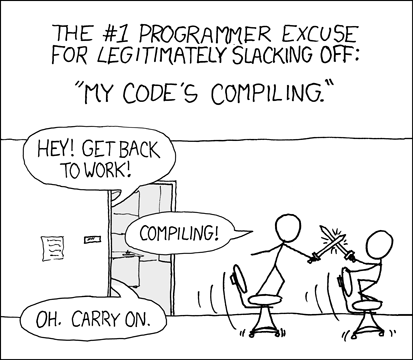
\includegraphics{compiling.png} \\
    \footnotesize\sffamily%
    Tiré de \href{http://xkcd.com/303/}{XKCD.com}
  \end{minipage}
  \setkeys{Gin}{width=0.8\textwidth}
\end{vplace}

\mainmatter

%%% Copyright (C) 2017 Vincent Goulet
%%%
%%% Ce fichier fait partie du projet «Programmer avec R»
%%% http://github.com/vigou3/programmer-avec-r
%%%
%%% Cette création est mise à disposition selon le contrat
%%% Attribution-Partage dans les mêmes conditions 4.0
%%% International de Creative Commons.
%%% http://creativecommons.org/licenses/by-sa/4.0/

\chapter{Éléments d'informatique pour programmeurs}
\label{chap:informatique}

Intro du chapitre

\section{Bref historique des langages de programmation}
\label{sec:informatique:historique}

Ada Lovelace (1815--1852) est généralement reconnue comme la première
auteure d'un algorithme et de ce que l'on appelle aujourd'hui un
programme informatique. C'est en son honneur qu'été nommé le langage
Ada conçu en réponse à un cahier de charges du département de la
Défense des États-Unis au début des années 1980.

Franchissons d'un bond les premiers jours de l'informatique et de la
programmation pour arriver aux ordinateurs électriques modernes, dans
les années 1940. On programme alors généralement ceux-ci en
\emph{assembleur}, un langage de très bas niveau facilement
interprétable par la machine, mais difficile à lire par des humains,
comme l'extrait de programme de la
\autoref{fig:informatique:assembleur} le démontre bien.

\begin{figure}
  \centering
  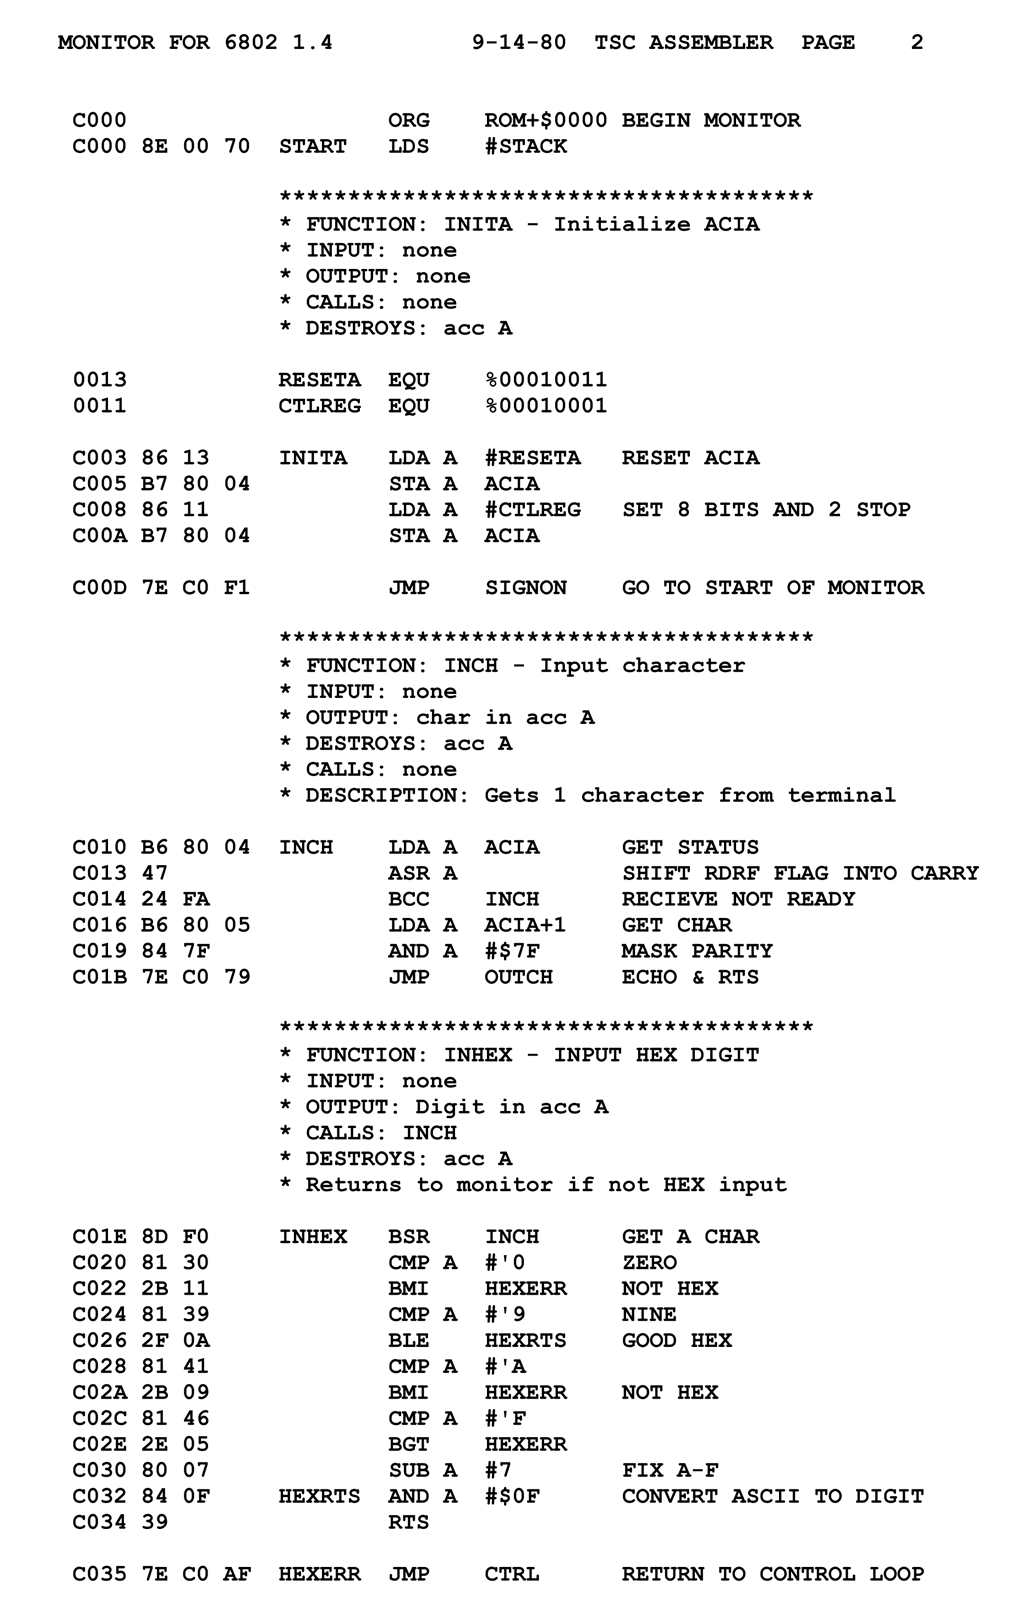
\includegraphics[trim=0 475 0 0, clip=true]{Motorola_6800_Assembly_Language.png}
  \caption[Programme en assembleur pour un microprocesseur 8~bits
  Motorola 6800.]{Extrait d'un programme en assembleur pour un
    microprocesseur 8~bits Motorola 6800. {\small Source:
      \link{https://commons.wikimedia.org/wiki/File\%3AMotorola_6800_Assembly_Language.png}{Wikimedia
        Commons}}}
  \label{fig:informatique:assembleur}
\end{figure}

Les premiers langages créés pour transmettre des instructions à un
ordinateur apparaissent dans les années 1950. Ils sont à l'origine
intimement liés à l'architecture d'un ordinateur: à chaque type
d'ordinateur son langage de programmation. Certaines contraintes ---
ou exigences --- des langages de l'époque proviennent aussi du support
physique alors utilisé pour stocker les programmes: les cartes
perforées.

\subsection{Fortran}
\label{sec:informatique:historique:fortran}

En 1954, l'ingénieur de IBM John Backus publie les spécifications du
langage FORTRAN (\emph{FORmula TRANslating System}). Le premier
compilateur voit le jour deux ans plus tard. Fortran (avec des
minuscules à partir de 1977) deviendra rapidement le langage standard
dans le calcul scientifique.

Plus d'un demi-siècle plus tard, l'empreinte de Fortran demeure
importante, notamment grâce aux bibliothèques d'algèbre linéaire
BLAS\footnote{%
  \emph{Basic Linear Algebra Subprograms};
  \link{http://www.netlib.org/blas}{}.} %
et LAPACK\footnote{%
  \emph{Linear Algebra PACKage};
  \link{http://www.netlib.org/lapack}{}.} %
auxquelles ont recours la plupart des progiciels scientifiques, dont
R. Le langage est toujours utilisé en calcul haute performance et pour
mesurer le rendement des superordinateurs.

\begin{figure}[t]
  \notebox{Dans le très recommandable film Les figures de l'ombre
    (\emph{Hidden Figures}, 2016), une des héroïnes entreprend de
    s'attaquer à la programmation des nouveaux ordinateurs de la NASA.
    On peut alors voir qu'elle apprend le Fortran.}
\end{figure}

\subsection{Lisp}
\label{sec:informatique:historique:lisp}

Le deuxième langage le plus ancien toujours largement diffusé est Lisp
(\emph{LISt Processing}). Créé par John McCarthy en 1958 en tant que
modèle pratique pour représenter des programmes, le Lisp est devenu le
langage de choix pour la recherche et les applications en intelligence
artificielle. Le terme Lisp désigne aujourd'hui une famille de
langages comprenant de nombreux dialectes, dont Common Lisp, Scheme et
Emacs Lisp.

Le Lisp se distingue en outre par une syntaxe simple en notation
préfixée (voir encadré), le support pour la programmation
fonctionnelle (\autoref{sec:informatique:paradigmes}) et la faculté de
manipuler le code source en tant que structure de données. Autre trait
distinctif: la syntaxe du Lisp fait un usage immodéré des parenthèses.

Le Lisp est entouré d'une aura de beauté et d'élégance dont peu
d'autres langages peuvent se targuer. Citons Eric Raymond dans
\link{http://www.catb.org/esr/faqs/hacker-howto.html}{\emph{How to
    Become a Hacker}}:
\begin{quote}
  Il faut apprendre le Lisp pour l'extraordinaire expérience d'éveil
  [\emph{enlightenment experience}] que procure le fait de finalement
  le comprendre; cette expérience fera de vous un meilleur programmeur
  pour toujours, même si vous n'avez plus vraiment à utiliser le Lisp.
\end{quote}

Pour illustrer encore davantage la place toute particulière qu'occupe
le Lisp en programmation, mentionnons également l'aphorisme selon
lequel «ceux qui ne connaissent pas le Lisp sont condamnés à le
réinventer», d'une certaine façon la version courte de la célèbre
\link{https://en.wikipedia.org/wiki/Greenspun\%27s_tenth_rule}{\emph{Greenspun's
    tenth rule of programming}}: %
\begin{quote}
  Tout programme en C ou en Fortran suffisamment complexe contient une
  implémentation mal spécifiée, pleine de bogues et lente de la moitié
  de Common Lisp.
\end{quote}
(Fait amusant à noter: il n'y a pas d'autres lois que la dixième, de
l'\link{http://philip.greenspun.com/bboard/q-and-a-fetch-msg?msg_id=000tgU}{aveu
  même de l'auteur}.)

\begin{figure}[t]
  \label{fig:informatique:notations}
  \setlength{\FrameRule}{1pt}
  \lstset{backgroundcolor=\color{codebg},
    frame=lr, rulecolor=\color{codebg},
    xleftmargin=3.4pt, xrightmargin=3.4pt}
  \begin{emphbox}{\mdseries Notations infixée, préfixée et suffixée}
    Les notations infixée (\emph{infix}), préfixée (\emph{prefix}) et
    suffixée (\emph{postfix}) sont trois manières différentes, mais
    équivalentes, d'écrire des expressions en mathématiques ou en
    programmation.

    Par exemple, l'opération d'addition de deux opérandes $x$ et $y$
    s'écrit en notation infixée
\begin{lstlisting}
x + y
\end{lstlisting}
    En notation préfixée, aussi appelée notation polonaise,
    l'opérateur est placé \emph{avant} les opérandes:
\begin{lstlisting}
+ x y
\end{lstlisting}
    On l'aura compris, en notation suffixée, ou notation polonaise
    inversée, l'opérateur apparait \emph{après} les opérandes:
\begin{lstlisting}
x y +
\end{lstlisting}
    Nous sommes davantage habitués à lire la notation infixée, quoique
    la notation préfixée nous soit familière pour les opérateurs à un
    seul opérande (comme la négation) ou pour les appels de fonctions.
    La notation suffixée n'a jamais recours aux parenthèses.

    La compagnie HP commercialise de très prisées calculatrices
    scientifiques utilisant la notation suffixée (libellées RPN pour
    \emph{Reverse Polish Notation}) depuis 1972.
  \end{emphbox}
\end{figure}

\subsection{COBOL}
\label{sec:informatique:historique:cobol}

Le troisième langage développé dans les années 1950 et toujours en
usage de nos jours est COBOL (\emph{COmmon Business Oriented
  Language}). Ce langage spécialisé dans les applications de gestion a
été créé en 1959 par un comité formé pour proposer un langage commun
pour l'administration américaine.

Le COBOL reste très utilisé dans de grandes entreprises, notamment
dans les institutions financières. La légende urbaine veut d'ailleurs
que les programmeurs COBOL soient comparativement très bien rémunérés
aujourd'hui sous l'effet combiné de leur rareté et de l'importance
opérationnelle des applications qu'ils doivent maintenir.

\subsection{Algol}
\label{sec:informatique:historique:algol}

Dès la fin de la décennie 1950, un comité de scientifiques se réunit à
Zurich pour concevoir ce que l'on voudrait voir devenir le langage de
programmation standard. De ces rencontres naîtra Algol
(\emph{ALGorithmic Oriented Language}) en 1958. Comme la plupart des
tentatives de définition d'un standard, c'est un échec: le langage est
populaire dans les milieux académiques, mais restera peu utilisé dans
les applications commerciales.

Cela dit, on doit à Algol plusieurs innovations importantes, de telle
sorte qu'un grand nombre des langages qui verront le jour par la suite
seront considérés comme ses descendants; le poster
\link{http://www.oreilly.com/go/languageposter}{\emph{History of
    Programming Languages}} de O'Reilly Media illustre ce fait à
merveille. \citet{Hoare:1973} a d'ailleurs cette jolie formule:
\begin{quote}
  Voici un langage très en avance sur son temps, il n'a pas seulement
  été une amélioration de ses prédécesseurs mais aussi une
  amélioration de presque tous ses successeurs.
\end{quote}


\begin{figure}[t]
  \centering
  \begin{minipage}{0.9\linewidth}
    \setkeys{Gin}{width=\textwidth}
    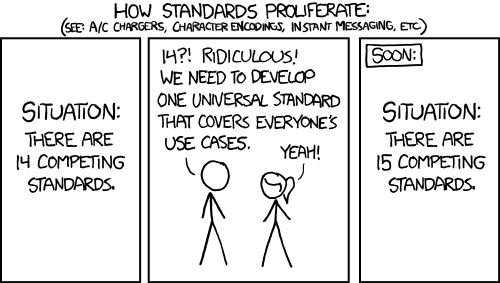
\includegraphics{standards} \\
    \footnotesize\sffamily%
    Tiré de \href{http://xkcd.com/927/}{XKCD.com}
  \end{minipage}
\end{figure}

\subsection{APL}
\label{sec:informatique:historique:apl}

Notre historique ne serait pas complet sans un mot sur APL (\emph{A
  Programming Language}, qui l'aurait cru). Même s'il n'a jamais connu
une diffusion importante, ce langage conçu par Kenneth Iverson autour
de 1962 n'en a pas moins eu une influence considérable sur la manière
de penser et de représenter les opérations mathématiques sur les
tableaux à plusieurs dimensions.

Doté d'une large gamme de symboles pour représenter des opérations et
d'une syntaxe tout à fait particulière --- les expressions sont
exécutées de droite à gauche! --- l'APL est remarquablement concis et
puissant; voir la \autoref{fig:informatique:apl} pour un aperçu. Le
revers de la cette médaille et ce qui a assurément nui à son adoption
à large échelle, c'est la difficulté que l'on éprouve à relire le
code. Assez pour que d'aucuns qualifient l'APL de «langage à écriture
seulement».

APL a pendant longtemps été un langage très prisé par les actuaires,
aussi subsiste-t-il du code dans certaines compagnies d'assurance. Le
modèle de traitement des vecteurs, matrices et tableaux de l'APL a
servi d'inspiration pour la conception du langage S --- nous y
reviendrons au \autoref{chap:presentation}.

Le langage continue sa vie aujourd'hui principalemnt sous forme de son
successeur, J.

\begin{figure}
  \centering
  \scalebox{0.4}{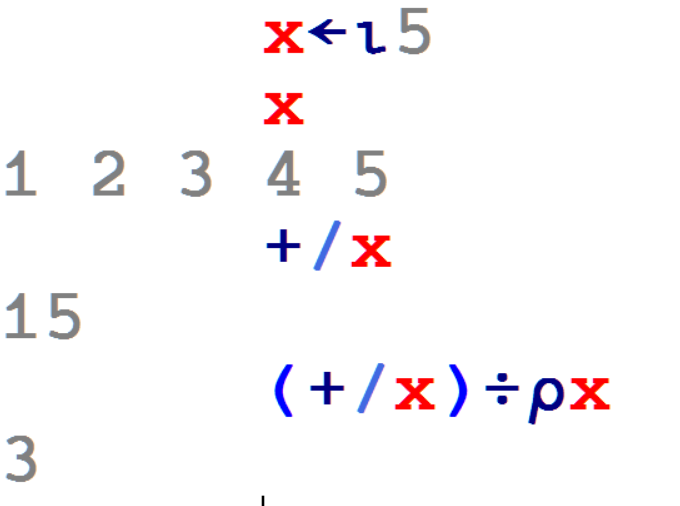
\includegraphics{APL_intro}}
  \caption[Opérations simples en APL.]{Opérations simples en APL. De
    haut en bas: génération des nombres de $1$ à $5$ et stockage dans
    la variable \code{x}; affichage du contenu de \code{x}; somme des
    éléments de \code{x}; moyenne des éléments de \code{x}. {\small Source:
    François-Dominique,
    \link{https://commons.wikimedia.org/w/index.php?curid=43207460}{Wikimedia
      Commons}, CC BY-SA 4.0}}
  \label{fig:informatique:apl}
\end{figure}

\subsection{C}
\label{sec:informatique:historique:c}

Le langage C a été inventé en 1972 chez Bell Labs par Ken Thompson et
Dennis Ritchie afin de réécrire le système d'exploitation UNIX
(\autoref{sec:informatique:os:unix}). Il demeure beaucoup utilisé pour
la programmation système: le noyau de systèmes d'exploitation comme
Windows et Linux sont développés en grande partie en C.

Le C est un langage de programmation généraliste considéré, selon les
standards actuels, comme de bas niveau. Pour illustrer, l'utilisateur
doit programmer des traitements comme la libération de la mémoire, la
vérification de la validité des indices sur les tableaux, l'ouverture
et la fermeture des fichiers, etc.

Le langage demeure l'un des plus utilisés dans le monde et son
influence est considérable. De nombreux langages plus modernes comme
\Cpp, C\# et Java reprennent des aspects de C. Le C est également
beaucoup utilisé pour le calcul numérique intensif, où il s'est en
quelque sorte substitué à Fortran. La plupart des progiciels
scientifiques --- dont R, encore une fois --- offrent la possibilité
d'appeler du code C lorsque la rapidité de calcul devient un enjeu. Le
gain en temps d'exécution doit toutefois être suffisamment grand pour
compenser le temps de développement plus long qu'exige le C par
rapport à des langages de plus haut niveau.

\begin{figure}[t]
  \notebox{Dans l'ouvrage désormais classique de \cite{KandR:1978}, le
    premier exemple d'un programme C affiche le message «\emph{hello,
      world}» à l'écran. Ça deviendra ensuite une tradition de
    démontrer le fonctionnement ou la syntaxe d'un langage avec cet
    exemple.}
\end{figure}

\subsection{Autres jalons}
\label{sec:informatique:historique:autres}

Nous nous sommes attardés jusqu'ici à des langages de programmation
vieux de plus de 40 ans à cause de leur importance historique et parce
qu'ils sont toujours utilisés couramment. De nombreux autres langages
ont vu le jour depuis, si bien qu'ils se comptent aujourd'hui par
milliers. En voici quelques autres ayant occupé une place
prépondérante dans l'histoire.

\begin{itemize}
\item Comme son nom l'indique, \textbf{\Cpp} (Bjarne Stroustrup, 1980)
  est un dérivé du C qui lui ajoute, en autres choses, la
  programmation orientée objet. Certains considèrent que {\Cpp}
  devrait être le point d'entrée de toute personne voulant débuter à
  programmer avec des langages de la famille du C. Le code C est
  compatible avec le \Cpp.
\item Principal représentant de l'ère Internet des années 1990,
  \textbf{Java} (James Gosling, 1995) a été conçu pour que le code
  écrit dans ce langage puisse s'exécuter sur n'importe quelle
  plateforme informatique sans nécessiter une nouvelle compilation. Il
  est donc très populaire dans les applications web ou embarquées. Sa
  syntaxe est fortement inspirée du \Cpp.
\item \textbf{Visual Basic} (Microsoft, 1991) permet de développer des
  applications de manière interactive en disposant des composantes sur
  un canevas. Le langage est aujourd'hui discontinué, mais son dérivé
  \textbf{Visual Basic for Applications} (VBA) demeure beaucoup
  utilisé dans les applications de la suite bureautique Office.
\item \textbf{Python} (Guido van Rossum, 1991) est un langage de haut
  niveau, orienté objet, multiplateforme et sous licence libre. C'est
  un des langages les plus utilisés aujourd'hui pour le calcul
  scientifique et l'analyse de données massives.
\end{itemize}

Certains langages de programmation ont une vocation généraliste,
certains visent des niches particulières, alors que d'autres cherchent
surtout à faire progresser l'état des connaissances dans la théorie
des langages. Quoi qu'il en soit, un langage de programmation demeure
un outil et, en informatique comme dans d'autres domaines, il convient
de choisir le meilleur outil pour accomplir une tâche donnée.

Nous invitons les lecteurs intéressés à en savoir davantage sur
l'histoire des langages de programmation en général, ou sur l'un ou
l'autre des langages mentionnés ci-dessus en particulier, à débuter
par les très complètes entrées de Wikipedia en
\link{https://fr.wikipedia.org/wiki/Histoire_des_langages_de_programmation}{français}
et en
\link{https://en.wikipedia.org/wiki/History_of_programming_languages}{anglais}.


\section{Sémantique et syntaxe}
\label{sec:informatique:semantique}

Il y a plusieurs parallèles à dresser entre les langages de
programmation et les langues parlées ou écrites: leur apprentissage
requiert de la pratique; on en connait jamais un trop grand nombre; le
premier est plus difficile à apprendre que les suivants.
L'informatique a également emprunté à la linguistique les notions de
\emph{sémantique} et de \emph{syntaxe}.

La sémantique est l'étude de ce que signifie un message ou un
programme informatique, c'est-à-dire de ce qu'il transmet ou exécute.
La syntaxe, quant à elle, étudie la structure du message ou du
programme. En simplifiant, disons que, pour une langue donnée, un
dictionnaire permet de connaître la sémantique, alors qu'une grammaire
décrit la syntaxe \citep{Hebenstreit:semantique}.

Par exemple, exprimons le message «J'ai soif» en anglais. Dire
«\emph{I am hungry}» relèverait d'une erreur de sémantique, puisque la
signification du message s'en trouve changée. En revanche, avec
«\emph{I have thirsty}» le bon message se rendra, mais peut-être pas
sans que l'erreur de syntaxe n'ait d'abord suscité une hésitation chez
l'interlocuteur.

Comme pour une langue, la maîtrise d'un langage de programmation exige
de respecter à la fois les règles de sémantique et les régles de
syntaxe du langage. Le second volet est relativement facile: si le
programme compile ou s'exécute, c'est généralement que la syntaxe est
respectée. Le respect de la sémantique, ou de la manière propre d'un
langage d'exprimer des idées, demande plus d'efforts et de pratique.


\section{Paradigmes de programmation}
\label{sec:informatique:paradigmes}

\section{Systèmes d'exploitation}
\label{sec:informatique:os}



%%% Local Variables:
%%% mode: latex
%%% TeX-engine: xetex
%%% TeX-master: "programmer-avec-r"
%%% End:

\chapter{Pr�sentation du langage S}
\label{presentation}


\section{Le langage S}
\label{presentation:langage}

Le S est un langage pour �programmer avec des donn�es� d�velopp� chez
Bell Laboratories (anciennement propri�t� de AT\&T, maintenant de
Lucent Technologies).

\begin{itemize}
\item Ce n'est pas seulement un �autre� environnement statistique
  (comme SPSS ou SAS, par exemple), mais bien un langage de
  programmation complet et autonome.
\item Inspir� de plusieurs langages, dont l'APL et le Lisp, le S est:
  \begin{itemize}
  \item interpr�t� (et non compil�);
  \item sans d�claration obligatoire des variables;
  \item bas� sur la notion de vecteur;
  \item particuli�rement puissant pour les applications math�matiques
    et statistiques (et donc actuarielles).
  \end{itemize}
\end{itemize}


\section{Les moteurs S}
\label{presentation:moteurs}

Il existe quelques �moteurs� ou dialectes du langage S.

\begin{itemize}
\item Le plus connu est S-Plus, un logiciel commercial de
  Insightful Corporation (Bell Labs octroie � Insightful la licence
  exclusive de son syst�me S).
\item \textsf{R}, ou GNU S, est une version libre (\emph{Open Source})
  �\emph{not unlike S}�.
\end{itemize}

S-Plus et \textsf{R} constituent tous deux des environnements int�gr�s
de manipulation de donn�es, de calcul et de pr�paration de graphiques.


\section{O� trouver de la documentation}
\label{presentation:doc}

S-Plus est livr� avec quatre livres (disponibles en format PDF depuis
le menu \texttt{Help} de l'interface graphique), mais aucun ne s'av�re
vraiment utile pour apprendre le langage S.

Plusieurs livres --- en versions papier ou �lectronique, gratuits ou
non --- ont �t� publi�s sur S-Plus et \textsf{R}. On trouvera des
listes exhaustives dans les sites de Insightful et du projet
\textsf{R}:
\begin{itemize}
\item \url{http://www.insightful.com/support/splusbooks.asp}
\item \url{http://www.r-project.org} (dans la section
  \texttt{Documentation}).
\end{itemize}

De plus, les ouvrages de \citet{Sprogramming,MASS} constituent des
r�f�rences sur le langage S devenues au cours des derni�res ann�es des
standards \emph{de facto}.


\section{Interfaces pour S-Plus et \textsf{R}}
\label{presentation:interfaces}

Provenant du monde Unix, tant S-Plus que \textsf{R} sont d'abord et
avant tout des applications en ligne de commande (\texttt{sqpe.exe} et
\texttt{rterm.exe} sous Windows).

\begin{itemize}
\item S-Plus poss�de toutefois une interface graphique �labor�e
  permettant d'utiliser le logiciel sans trop conna�tre le langage de
  programmation.
\item \textsf{R} dispose �galement d'une interface graphique
  rudimentaire sous Windows et Mac OS.
\item L'�dition s�rieuse de code S b�n�ficie cependant grandement d'un
  bon �diteur de texte.
\item � la question 6.2 de la foire aux questions (FAQ) de \textsf{R},
  �Devrais-je utiliser \textsf{R} � l'int�rieur de
  Emacs?�\index{Emacs}, la r�ponse est: �Oui, absolument.� Nous
  partageons cet avis, aussi ce document supposera-t-il que S-Plus ou
  \textsf{R} sont utilis�s � l'int�rieur de GNU Emacs avec le mode
  ESS\index{ESS}.
\item Autre option: WinEdt (partagiciel) avec l'ajout R-WinEdt.
\end{itemize}


\section{Installation de Emacs avec ESS}
\label{presentation:emacs}

Il n'existe pas de proc�dure d'installation similaire aux autres
applications Windows pour Emacs.  L'installation n'en demeure pas
moins tr�s simple: il suffit de d�compresser un ensemble de fichiers
au bon endroit.

\begin{itemize}
\item Pour une installation simplifi�e de Emacs et ESS, consulter le
  site Internet
  \begin{quote}
    \url{http://vgoulet.act.ulaval.ca/pub/emacs/}
  \end{quote}
  On y trouve une version modifi�e de GNU Emacs et des instructions
  d'installation d�taill�es.
\item L'annexe \ref{ess} pr�sente les plus importantes commandes �
  conna�tre pour utiliser Emacs et le mode ESS.
\end{itemize}


\section{D�marrer et quitter S-Plus ou \textsf{R}}
\label{presentation:demarrer}

On suppose ici que S-Plus ou R sont utilis�s � l'int�rieur de Emacs.

\begin{itemize}
\item Pour d�marrer \textsf{R} \R � l'int�rieur de Emacs:
\begin{verbatim}
M-x R RET
\end{verbatim}
  puis sp�cifier un dossier de travail (voir la section
  \ref{presentation:workspace}). Une console \textsf{R} est ouverte
  dans une fen�tre (\emph{buffer} dans la terminologie de Emacs)
  nomm�e \texttt{*R*}.
\item Pour d�marrer S-Plus sous Windows, \Splus la proc�dure est
  similaire, sauf que la commande � utiliser est
\begin{verbatim}
M-x Sqpe RET
\end{verbatim}
  Consulter l'annexe \ref{s-plus_windows} pour de plus amples
  d�tails.
\item Pour quitter, deux options sont disponibles:
  \begin{enumerate}
  \item Taper \fonction{q()} � la ligne de commande.
  \item Dans Emacs, faire \ess{C-c C-q}. ESS va alors s'occuper de
    fermer le processus S ainsi que tous les \emph{buffers} associ�s �
    ce processus.
  \end{enumerate}
\end{itemize}


\section{Strat�gies de travail}
\label{presentation:strategies}

Il existe principalement deux fa�ons de travailler avec S-Plus et
\textsf{R}.
\begin{enumerate}
\item Le code est virtuel et les objets sont r�els. C'est l'approche
  qu'encouragent les interfaces graphiques, mais c'est aussi la moins
  pratique � long terme. On entre des expressions directement � la
  ligne de commande pour les �valuer imm�diatement.
\begin{Schunk}
\begin{Sinput}
> 2 + 3
\end{Sinput}
\begin{Soutput}
[1] 5
\end{Soutput}
\begin{Sinput}
> -2 * 7
\end{Sinput}
\begin{Soutput}
[1] -14
\end{Soutput}
\begin{Sinput}
> exp(1)
\end{Sinput}
\begin{Soutput}
[1] 2.718282
\end{Soutput}
\begin{Sinput}
> log(exp(1))
\end{Sinput}
\begin{Soutput}
[1] 1
\end{Soutput}
\end{Schunk}
  Les objets cr��s au cours d'une session de travail sont sauvegard�s.
  Par contre, � moins d'avoir �t� sauvegard� dans un fichier, le code
  utilis� pour cr�er ces objets est perdu lorsque l'on quitte S-Plus
  ou \textsf{R}.
\item Le code est r�el et les objets sont virtuels. C'est l'approche
  que nous favorisons. Le travail se fait essentiellement dans des
  fichiers de script (de simples fichiers de texte) dans lesquels sont
  sauvegard�es les expressions (parfois complexes!) et le code des
  fonctions personnelles. Les objets sont cr��s au besoin en ex�cutant
  le code. Emacs permet ici de passer efficacement des fichiers de
  script � l'ex�cution du code:
  \begin{enumerate}[i)]
  \item d�marrer un processus S-Plus (\texttt{M-x Sqpe}) ou
    \textsf{R} (\texttt{M-x R}) et sp�cifier le dossier de travail;
  \item ouvrir un fichier de script avec \ess{C-x C-f}. Pour cr�er un
    nouveau fichier, ouvrir un fichier inexistant;
  \item positionner le curseur sur une expression et faire \ess{C-c
      C-n} pour l'�valuer;
  \item le r�sultat appara�t dans le \emph{buffer} \texttt{*S+6*} ou
    \texttt{*R*}.
  \end{enumerate}
\end{enumerate}


\section{Gestion des projets ou environnements de travail}
\label{presentation:workspace}

S-Plus et \textsf{R} ont une mani�re diff�rente mais tout aussi
particuli�re de sauvegarder les objets cr��s au cours d'une session de
travail.
\begin{itemize}
\item Tous deux doivent travailler dans un dossier et non avec des
  fichiers individuels.
\item Dans S-Plus, \Splus tout objet cr�� au cours d'une session de
  travail est sauvegard� de fa�on permanente sur le disque dur dans le
  sous-dossier \texttt{\_\_Data} du dossier de travail.
\item Dans \textsf{R}, \R les objets cr��s sont conserv�s en m�moire
  jusqu'� ce que l'on quitte l'application ou que l'on enregistre le
  travail avec la commande \fonction{save.image()}. L'environnement de
  travail (\emph{workspace}) est alors sauvegard� dans le fichier
  \texttt{.RData} du dossier de travail.
\end{itemize}

Le dossier de travail est d�termin� au lancement de l'application.
\begin{itemize}
\item Avec Emacs et ESS, on doit sp�cifier le dossier de travail
  chaque fois que l'on d�marre un processus S-Plus ou R.
\item Les interfaces graphiques permettent �galement de sp�cifier le
  dossier de travail.
  \begin{itemize}
    \sloppy
  \item Dans \Splus l'interface graphique de S-Plus, choisir
    \texttt{General Settings} dans le menu \texttt{Options}, puis
    l'onglet \texttt{Startup}. Cocher la case \texttt{Prompt for
      project folder}.  Consulter �galement le chapitre 13 du guide de
    l'utilisateur de S-Plus.
  \item Dans \R l'interface graphique de \textsf{R}, le plus simple
    consiste � changer le dossier de travail � partir du menu
    \texttt{Fichier|Changer le r�pertoire courant...} Consulter aussi
    la \emph{R for Windows FAQ}.
  \end{itemize}
\end{itemize}


\section{Consulter l'aide en ligne}
\label{presentation:aide}

Les rubriques d'aide des diverses fonctions disponibles dans S-Plus et
\textsf{R} contiennent une foule d'informations ainsi que des exemples
d'utilisation. Leur consultation est tout � fait essentielle.

\begin{itemize}
\item Pour consulter la rubrique d'aide de la fonction \code{foo},
  on peut entrer � la ligne de commande
\begin{Schunk}
\begin{Sinput}
> ?foo
\end{Sinput}
\end{Schunk}
\item Dans Emacs, \code{C-c C-v foo RET}\indexess{C-c C-v} ouvrira la
  rubrique d'aide de la fonction \code{foo} dans un nouveau
  \emph{buffer}.
\item Plusieurs touches de raccourcis facilitent la consultation des
  rubriques d'aide (voir la carte de r�f�rence ESS).
\item Entre autres, la touche \texttt{l} permet d'ex�cuter ligne par
  ligne les exemples se trouvant � la fin de chaque rubrique d'aide.
\end{itemize}


\section{Exemples}
\label{presentation:exemples}

\lstinputlisting{presentation.R}


\section{Exercices}
\label{presentation:exercices}

\begin{exercice}
  D�marrer un processus S-Plus ou \textsf{R} � l'int�rieur de Emacs.
\end{exercice}

\begin{exercice}
  Ex�cuter un � un les exemples de la section pr�c�dente. Une version
  �lectronique du code de cette section est disponible dans le site
  mentionn� dans la pr�face.
\end{exercice}

\begin{exercice}
  Consulter les rubriques d'aide d'une ou plusieurs des fonctions
  rencontr�es lors de l'exercice pr�c�dent. Observer d'abord comment
  les ru\-bri\-ques d'aide sont structur�es --- elles sont toutes
  identiques --- puis ex�cuter quelques lignes d'exemples.
\end{exercice}

\begin{exercice}
  Lire le chapitre 1 de \cite{MASS} et ex�cuter les commandes de
  l'exemple de session de travail de la section 1.3. Bien que
  davantage orient� vers les application statistiques que vers la
  programmation, cet exemple d�montre quelques-unes des possibilit�s
  du langage S.
\end{exercice}

%%% Local Variables:
%%% mode: latex
%%% TeX-master: "introduction_programmation_S"
%%% End:

% \chapter{Bases du langage S}
\label{bases}


Ce chapitre pr�sente les bases du langage S, soit les notions
d'expression et d'affectation, la description d'un objet S et les
mani�res de cr�er les objets les plus usuels lorsque le S est utilis�
comme langage de programmation.

\section{Commandes S}
\label{bases:commandes}

Toute commande S est soit une \emph{expression}\index{expression},
soit une \emph{affectation}\index{affectation}.
\begin{itemize}
\item Normalement, une expression est imm�diatement �valu�e et le
  r�sultat est affich� � l'�cran:
\begin{Schunk}
\begin{Sinput}
> 2 + 3
\end{Sinput}
\begin{Soutput}
[1] 5
\end{Soutput}
\begin{Sinput}
> pi
\end{Sinput}
\begin{Soutput}
[1] 3.141593
\end{Soutput}
\begin{Sinput}
> cos(pi/4)
\end{Sinput}
\begin{Soutput}
[1] 0.7071068
\end{Soutput}
\end{Schunk}
\item Lors d'une affectation, une expression est �valu�e, mais le
  r�sultat est stock� dans un objet (variable) et rien n'est affich� �
  l'�cran. Le symbole d'affectation est \Fonction{<-} (ou
  \Fonction{->}).
\begin{Schunk}
\begin{Sinput}
> a <- 5
> a
\end{Sinput}
\begin{Soutput}
[1] 5
\end{Soutput}
\begin{Sinput}
> b <- a
> b
\end{Sinput}
\begin{Soutput}
[1] 5
\end{Soutput}
\end{Schunk}
\item �viter d'utiliser l'op�rateur \fonction{=} pour affecter une
  valeur � une variable, puisqu'il ne fonctionne que dans certaines
  situations seulement.
\item Dans S-Plus (mais plus dans \textsf{R} depuis la version 1.8.0),
  on peut �galement affecter avec le caract�re �\fonction{\_}�, mais cet
  emploi est fortement d�courag� puisqu'il rend le code difficile �
  lire. Dans le mode ESS de Emacs, taper ce caract�re g�n�re carr�ment
  \verb*| <- |.
\end{itemize}

\begin{astuce}
  Il arrive fr�quemment que l'on souhaite affecter le r�sultat d'un
  calcul dans un objet et en m�me temps voir ce r�sultat. Pour ce
  faire, placer l'affectation entre parenth�ses (l'op�ration
  d'affectation devient alors une nouvelle expression):
\begin{Schunk}
\begin{Sinput}
> (a <- 2 + 3)
\end{Sinput}
\begin{Soutput}
[1] 5
\end{Soutput}
\end{Schunk}
\end{astuce}


\section{Conventions pour les noms d'objets}
\index{noms d'objets!conventions}
\label{bases:noms}

Les caract�res permis pour les noms d'objets sont les lettres a--z,
A--Z, les chiffres 0--9 et le point �.�. Le caract�re \R �\code{\_}�
est maintenant permis dans \textsf{R}, mais son utilisation est
d�courag�e.

\begin{itemize}
\item Les noms d'objets ne peuvent commencer par un chiffre.
\item Le S est sensible � la casse, ce qui signifie que \code{foo},
  \code{Foo} et \code{FOO} sont trois objets distincts. Un moyen
  simple d'�viter des erreurs li�es � la casse consiste � n'employer
  que des lettres minuscules.
\item Certains noms sont utilis�s par le syst�me, aussi vaut-il mieux
  �viter de les utiliser. En particulier, �viter d'utiliser
  \begin{center}
    \code{c}, \code{q}, \code{t}, \code{C}, \code{D},
    \code{I}, \code{diff}, \code{length}, \code{mean},
    \code{pi}, \code{range}, \code{var}.
  \end{center}
\item \index{noms d'objets!r�serv�s} Certains mots sont r�serv�s pour
  le syst�me et il est interdit de les utiliser comme nom d'objet. Les
  mots r�serv�s sont:
  \begin{center}
    \code{Inf}, \code{NA}, \code{NaN},
    \code{NULL} \\
    \code{break}, \code{else},
    \code{for}, \code{function}, \code{if}, \code{in},
    \code{next}, \code{repeat}, \code{return}, \code{while}.
  \end{center}
\item Dans S-Plus 6.1 et plus, \Splus
  \code{T}\index{T@\code{T}|see{\code{TRUE}}} et \objet{TRUE} (vrai),
  ainsi que \code{F}\index{F@\code{F}|see{\code{FALSE}}} et
  \objet{FALSE} (faux) sont �galement des noms r�serv�s.
\item Dans \textsf{R}, \R les noms \code{TRUE} et \code{FALSE}
  sont �galement r�serv�s. Les variables \code{T} et \code{F}
  prennent par d�faut les valeurs \code{TRUE} et \code{FALSE},
  respectivement, mais peuvent �tre r�affect�es.
\begin{Schunk}
\begin{Sinput}
> T
\end{Sinput}
\begin{Soutput}
[1] TRUE
\end{Soutput}
\end{Schunk}
\begin{Schunk}
\begin{Sinput}
> TRUE <- 3
\end{Sinput}
\end{Schunk}
\begin{Schunk}
\begin{Soutput}
Erreur dans TRUE <- 3 : membre gauche de
l'assignation (do_set) incorrect
\end{Soutput}
\end{Schunk}
\begin{Schunk}
\begin{Sinput}
> (T <- 3)
\end{Sinput}
\begin{Soutput}
[1] 3
\end{Soutput}
\end{Schunk}
\end{itemize}


\section{Les objets S}
\label{bases:objets}

Tout dans le langage S est un objet, m�me les fonctions et les
op�rateurs. Les objets poss�dent au minimum un \emph{mode} et une
\emph{longueur}.

\begin{itemize}
\item Le mode d'un objet est obtenu avec la fonction \Fonction{mode}.
\begin{Schunk}
\begin{Sinput}
> v <- c(1, 2, 5, 9)
> mode(v)
\end{Sinput}
\begin{Soutput}
[1] "numeric"
\end{Soutput}
\end{Schunk}
\item La longueur d'un objet est obtenue avec la fonction
  \Fonction{length}.
\begin{Schunk}
\begin{Sinput}
> length(v)
\end{Sinput}
\begin{Soutput}
[1] 4
\end{Soutput}
\end{Schunk}
\item Certains objets sont �galement dot�s d'un ou plusieurs
  \emph{attributs}.
\end{itemize}


\subsection{Modes et types de donn�es}

Le mode\Index{mode} prescrit ce qu'un objet peut contenir. � ce titre,
un objet ne peut avoir qu'un seul mode. Le tableau \ref{tab:modes}
contient la liste des modes disponibles en S. � chacun de ces modes
correspond une fonction du m�me nom servant � cr�er un objet de ce
mode.

\begin{table}
  \centering
  \begin{tabular}{ll}
    \toprule
    \Mode{numeric}   & nombres r�els \\
    \Mode{complex}   & nombres complexes \\
    \Mode{logical}   & valeurs bool�ennes (vrai/faux) \\
    \Mode{character} & cha�nes de caract�res \\
    \Mode{function}  & fonction \\
    \Mode{list}      & donn�es quelconques \\
    \bottomrule
  \end{tabular}
  \caption{Modes disponibles et contenus correspondants}
  \label{tab:modes}
\end{table}

\subsection{Longueur}

La longueur\Index{longueur} d'un objet est �gale au nombre d'�l�ments
qu'il contient.

\begin{itemize}
\item La longueur d'une cha�ne de caract�res est toujours 1. Un
  objet de mode \code{character} doit contenir plusieurs cha�nes
  de caract�res pour que sa longueur soit sup�rieure � 1.
\begin{Schunk}
\begin{Sinput}
> v <- "actuariat"
> length(v)
\end{Sinput}
\begin{Soutput}
[1] 1
\end{Soutput}
\begin{Sinput}
> v <- c("a", "c", "t", "u", "a", "r", "i", 
+     "a", "t")
> length(v)
\end{Sinput}
\begin{Soutput}
[1] 9
\end{Soutput}
\end{Schunk}
\item Un objet peut �tre de longueur 0 et doit alors �tre interpr�t�
  comme un contenant vide\index{vide|see{\code{NULL}}}.
\begin{Schunk}
\begin{Sinput}
> v <- numeric(0)
> length(v)
\end{Sinput}
\begin{Soutput}
[1] 0
\end{Soutput}
\end{Schunk}
\end{itemize}


\subsection{Attributs}

Les attributs\Index{attribut} d'un objet sont des �l�ments
d'information additionnels li�s � cet objet. La liste des attributs
les plus fr�quemment rencontr�s se trouve au tableau
\ref{tab:attributs}. Pour chaque attribut, il existe une fonction du
m�me nom servant � extraire l'attribut correspondant d'un objet.

\begin{table}
  \centering
  \begin{tabular}{ll}
    \toprule
    \Attribut{class}    &
    affecte le comportement d'un objet \\
    \Attribut{dim}      &
    dimensions\index{dimension} des matrices et tableaux \\
    \Attribut{dimnames} &
    �tiquettes\index{etiquette@�tiquette} des dimensions des matrices
    et tableaux \\
    \Attribut{names}    &
    �tiquettes des �l�ments d'un objet \\
    \bottomrule
  \end{tabular}
  \caption{Attributs les plus usuels d'un objet et leur effet}
  \label{tab:attributs}
\end{table}


\subsection{L'objet sp�cial \code{NA}}

\Objet{NA} est fr�quemment utilis� pour repr�senter les donn�es
manquantes.

\begin{itemize}
\item Son mode est \mode{logical}.
\item Toute op�ration impliquant une donn�e \code{NA} a comme
  r�sultat \code{NA}.
\item Certaines fonctions (\fonction{sum}, \fonction{mean}, par
  exemple) ont par cons�quent un argument \Argument{na.rm} qui,
  lorsque \code{TRUE}, �limine les donn�es manquantes avant de
  faire un calcul.
\item La fonction \Fonction{is.na} permet de tester si les �l�ments
  d'un objet sont \code{NA} ou non.
\end{itemize}

\subsection{L'objet sp�cial \code{NULL}}

\Objet{NULL} repr�sente �rien�, ou le vide.

\begin{itemize}
\item Son mode est \Mode{NULL}.
\item Sa longueur est 0.
\item Diff�rent d'un objet vide:
  \begin{itemize}
  \item un objet de longueur 0 est un contenant vide;
  \item \code{NULL} est �pas de contenant�.
  \end{itemize}
\item La fonction \Fonction{is.null} teste si un objet est \code{NULL}
  ou non.
\end{itemize}


\section{Vecteurs}
\label{bases:vecteurs}

En S, � peu de choses pr�s, \emph{tout} est un vecteur\index{vecteur}.
(Il n'y a pas de notion de scalaire.)

\begin{itemize}
\item Dans un vecteur simple, tous les �l�ments doivent �tre du
  m�me mode.
\item Il est possible (et souvent souhaitable) de donner une �tiquette
  � chacun des �l�ments d'un vecteur.
\begin{Schunk}
\begin{Sinput}
> (v <- c(a = 1, b = 2, c = 5))
\end{Sinput}
\begin{Soutput}
a b c 
1 2 5 
\end{Soutput}
\begin{Sinput}
> v <- c(1, 2, 5)
> names(v) <- c("a", "b", "c")
> v
\end{Sinput}
\begin{Soutput}
a b c 
1 2 5 
\end{Soutput}
\end{Schunk}
\item Les fonctions de base pour cr�er des vecteurs sont:
  \begin{itemize}
  \item \Fonction{c} (concat�nation);
  \item \Fonction{numeric} (vecteur de mode \mode{numeric});
  \item \Fonction{logical} (vecteur de mode \mode{logical});
  \item \Fonction{character} (vecteur de mode \mode{character}).
  \end{itemize}
\item L'indi�age dans un vecteur se fait avec \fonction{[\ ]}. On
  peut extraire un �l�ment d'un vecteur par sa position ou par son
  �tiquette, si elle existe (auquel cas cette approche est beaucoup
  plus s�re).
\begin{Schunk}
\begin{Sinput}
> v[3]
\end{Sinput}
\begin{Soutput}
c 
5 
\end{Soutput}
\begin{Sinput}
> v["c"]
\end{Sinput}
\begin{Soutput}
c 
5 
\end{Soutput}
\end{Schunk}
  La section \ref{bases:indicage} traite plus en d�tail de l'indi�age de
  vecteurs et matrices.
\end{itemize}


\section{Matrices et tableaux}
\label{bases:matrices}

Une matrice\index{matrice} ou, de fa�on plus g�n�rale, un
tableau\index{tableau} (\emph{array}) n'est rien d'autre qu'un vecteur
dot� d'un attribut \attribut{dim}. � l'interne, une matrice est donc
stock�e sous forme de vecteur.

\begin{itemize}
\item La fonction de base pour cr�er des matrices est
  \Fonction{matrix}.
\item La fonction de base pour cr�er des tableaux est
  \Fonction{array}.
\item \emph{Important}: \warning les matrices et tableaux sont remplis
  en faisant d'abord varier la premi�re dimension, puis la seconde,
  etc. Pour les matrices, cela revient � remplir par colonne.
\begin{Schunk}
\begin{Sinput}
> matrix(1:6, nrow = 2, ncol = 3)
\end{Sinput}
\begin{Soutput}
     [,1] [,2] [,3]
[1,]    1    3    5
[2,]    2    4    6
\end{Soutput}
\begin{Sinput}
> matrix(1:6, nrow = 2, ncol = 3, byrow = TRUE)
\end{Sinput}
\begin{Soutput}
     [,1] [,2] [,3]
[1,]    1    2    3
[2,]    4    5    6
\end{Soutput}
\end{Schunk}
\item L'indi�age \index{indi�age!matrice} d'une matrice se fait
  �galement avec \fonction{[\ ]}. On extrait les �l�ments en pr�cisant
  leurs positions sous la forme (ligne, colonne) dans la matrice, ou
  encore leurs positions dans le vecteur sous-jacent.
\begin{Schunk}
\begin{Sinput}
> (m <- matrix(c(40, 80, 45, 21, 55, 32), 
+     nrow = 2, ncol = 3))
\end{Sinput}
\begin{Soutput}
     [,1] [,2] [,3]
[1,]   40   45   55
[2,]   80   21   32
\end{Soutput}
\begin{Sinput}
> m[1, 2]
\end{Sinput}
\begin{Soutput}
[1] 45
\end{Soutput}
\begin{Sinput}
> m[3]
\end{Sinput}
\begin{Soutput}
[1] 45
\end{Soutput}
\end{Schunk}
\item La fonction \Fonction{rbind} permet de fusionner verticalement
  deux matrices (ou plus) ayant le m�me nombre de colonnes.
\begin{Schunk}
\begin{Sinput}
> n <- matrix(1:9, nrow = 3)
> rbind(m, n)
\end{Sinput}
\begin{Soutput}
     [,1] [,2] [,3]
[1,]   40   45   55
[2,]   80   21   32
[3,]    1    4    7
[4,]    2    5    8
[5,]    3    6    9
\end{Soutput}
\end{Schunk}
\item La fonction \Fonction{cbind} permet de fusionner horizontalement
  deux matrices (ou plus) ayant le m�me nombre de lignes.
\begin{Schunk}
\begin{Sinput}
> n <- matrix(1:4, nrow = 2)
> cbind(m, n)
\end{Sinput}
\begin{Soutput}
     [,1] [,2] [,3] [,4] [,5]
[1,]   40   45   55    1    3
[2,]   80   21   32    2    4
\end{Soutput}
\end{Schunk}
\end{itemize}


\section{Listes}
\label{bases:listes}

Une liste\index{liste} est un type de vecteur sp�cial dont les
�l�ments peuvent �tre de n'importe quel mode, y compris le mode
\mode{list} (ce qui permet d'embo�ter des listes).

\begin{itemize}
\item La fonction de base pour cr�er des listes est \Fonction{list}.
\item Il est g�n�ralement pr�f�rable de nommer les �l�ments d'une
  liste. Il est en effet plus simple et s�r d'extraire les �l�ments
  par leur �tiquette.
\item L'extraction\Index{indi�age!liste} des �l�ments d'une liste peut
  se faire de deux fa�ons:
  \begin{enumerate}
  \item avec des doubles crochets \fonction{[[\ ]]};
  \item par leur �tiquette avec \code{nom.liste\$etiquette.element}.
  \end{enumerate}
\item La fonction \Fonction{unlist} convertit une liste en un vecteur
  simple. Attention, cette fonction peut �tre destructrice si la
  structure de la liste est importante.
\end{itemize}


\section{\emph{Data frames}}
\label{bases:dataframes}

Les vecteurs, matrices, tableaux (\emph{arrays}) et listes sont les
types d'objets les plus fr�quemment utilis�s en S pour la
programmation de fonctions personnelles ou la simulation. L'analyse de
donn�es --- la r�gression lin�aire, par exemple --- repose toutefois
davantage sur les \emph{data frames}\Index{data frame}.

\begin{itemize}
\item Un \emph{data frame} est une liste de classe \classe{data.frame}
  dont tous les �l�ments sont de la m�me longueur.
\item G�n�ralement repr�sent� sous la forme d'un tableau � deux
  dimensions (visuellement similaire � une matrice). Chaque �l�ment de
  la liste sous-jacente correspond � une colonne.
\item On peut donc obtenir les �tiquettes des colonnes avec la fonction
  \fonction{names} (ou \fonction{colnames} \R dans \textsf{R}).  Les
  �tiquettes des lignes sont quant � elles obtenues avec
  \fonction{row.names} (ou \fonction{rownames} dans \textsf{R}).
\item Plus g�n�ral qu'une matrice puisque les colonnes peuvent �tre de
  modes diff�rents (\mode{numeric}, \mode{complex}, \mode{character}
  ou \mode{logical}).
\item Peut �tre indic� � la fois comme une liste et comme une matrice.
\item Cr�� avec la fonction \Fonction{data.frame} ou
  \Fonction{as.data.frame} (pour convertir une matrice en \emph{data
    frame}, par exemple).
\item Les fonctions \fonction{rbind} et \fonction{cbind} peuvent �tre
  utilis�es pour ajouter des lignes ou des colonnes, respectivement.
\item On peut rendre les colonnes d'un \emph{data frame} (ou d'une
  liste) visibles dans l'espace de travail avec la fonction
  \Fonction{attach}, puis les masquer avec \Fonction{detach}.
\end{itemize}

Ce type d'objet est moins important lors de l'apprentissage du langage
de programmation.




\section{Indi�age}
\label{bases:indicage}

L'indi�age des vecteurs\Index{indi�age!vecteur} et
matrices\Index{indi�age!matrice} a d�j� �t� bri�vement pr�sent� aux
sections \ref{bases:vecteurs} et \ref{bases:matrices}. La pr�sente
section contient plus de d�tails sur cette proc�dure des plus communes
lors de l'utilisation du langage S. On se concentre toutefois sur le
traitement des vecteurs. Se r�f�rer �galement � \citet[section
2.3]{MASS} pour de plus amples renseignements.

Il existe quatre fa�ons d'indicer un vecteur dans le langage S. Dans
tous les cas, l'indi�age se fait � l'int�rieur de crochets \Fonction{[\ ]}.
\begin{enumerate}
\item Avec un vecteur d'entiers positifs. Les �l�ments se trouvant aux
  positions correspondant aux entiers sont extraits du vecteur, dans
  l'ordre. C'est la technique la plus courante.
\begin{Schunk}
\begin{Sinput}
> letters[c(1:3, 22, 5)]
\end{Sinput}
\begin{Soutput}
[1] "a" "b" "c" "v" "e"
\end{Soutput}
\end{Schunk}
\item Avec un vecteur d'entiers n�gatifs. Les �l�ments se trouvant aux
  positions correspondant aux entiers n�gatifs sont alors
  \emph{�limin�s} du vecteur.
\begin{Schunk}
\begin{Sinput}
> letters[c(-(1:3), -5, -22)]
\end{Sinput}
\begin{Soutput}
 [1] "d" "f" "g" "h" "i" "j" "k" "l" "m" "n" "o" "p"
[13] "q" "r" "s" "t" "u" "w" "x" "y" "z"
\end{Soutput}
\end{Schunk}
\item Avec un vecteur bool�en. Le vecteur d'indi�age doit alors �tre
  de la m�me longueur que le vecteur indic�. Les �l�ments
  correspondant � une valeur \code{TRUE} sont extraits du vecteur,
  alors que ceux correspondant � \code{FALSE} sont �limin�s.
\begin{Schunk}
\begin{Sinput}
> letters > "f" & letters < "q"
\end{Sinput}
\begin{Soutput}
 [1] FALSE FALSE FALSE FALSE FALSE FALSE  TRUE  TRUE
 [9]  TRUE  TRUE  TRUE  TRUE  TRUE  TRUE  TRUE  TRUE
[17] FALSE FALSE FALSE FALSE FALSE FALSE FALSE FALSE
[25] FALSE FALSE
\end{Soutput}
\begin{Sinput}
> letters[letters > "f" & letters < "q"]
\end{Sinput}
\begin{Soutput}
 [1] "g" "h" "i" "j" "k" "l" "m" "n" "o" "p"
\end{Soutput}
\end{Schunk}
\item Avec une cha�ne de caract�res. Utile pour extraire les �l�ments
  d'un vecteur � condition que ceux-ci soient nomm�s.
\begin{Schunk}
\begin{Sinput}
> x <- c(Rouge = 2, Bleu = 4, Vert = 9, Jaune = -5)
> x[c("Bleu", "Jaune")]
\end{Sinput}
\begin{Soutput}
 Bleu Jaune 
    4    -5 
\end{Soutput}
\end{Schunk}
\end{enumerate}


\section{Exemples}
\label{bases:exemples}

\lstinputlisting{bases.R}


\section{Exercices}
\label{bases:exercices}

\Opensolutionfile{reponses}[reponses-bases]
\Writetofile{reponses}{\protect\section*{Chapitre \protect\ref{bases}}}

\begin{exercice}
  \begin{enumerate}
  \item �crire une expression S pour cr�er la liste suivante:
\begin{Schunk}
\begin{Soutput}
[[1]]
[1] 1 2 3 4 5

$data
     [,1] [,2] [,3]
[1,]    1    3    5
[2,]    2    4    6

[[3]]
[1] 0 0 0

$test
[1] FALSE FALSE FALSE FALSE
\end{Soutput}
\end{Schunk}
  \item \index{etiquette@�tiquette} Extraire les �tiquettes de la
    liste.
  \item \index{mode} \index{longueur} Trouver le mode et la longueur
    du quatri�me �l�ment de la liste.
  \item \index{dimension} Extraire les dimensions du second �l�ment de
    la liste.
  \item \index{indi�age!liste} Extraire les deuxi�me et troisi�me
    �l�ments du second �l�ment de la liste.
  \item Remplacer le troisi�me �l�ment de la liste par le vecteur
    \verb|3:8|.
  \end{enumerate}
  \begin{rep}
    Soit \code{x} le nom de la liste.
    \begin{enumerate}
\item
\begin{Schunk}
\begin{Sinput}
> list(1:5, data = matrix(1:6, 2, 3), numeric(3), 
+     test = logical(4))
\end{Sinput}
\end{Schunk}
\item
\begin{Schunk}
\begin{Sinput}
> names(x)
\end{Sinput}
\end{Schunk}
\item
\begin{Schunk}
\begin{Sinput}
> mode(x$test)
> length(x$test)
\end{Sinput}
\end{Schunk}
\item
\begin{Schunk}
\begin{Sinput}
> dim(x$data)
\end{Sinput}
\end{Schunk}
\item
\begin{Schunk}
\begin{Sinput}
> x[[2]][c(2, 3)]
\end{Sinput}
\end{Schunk}
\item
\begin{Schunk}
\begin{Sinput}
> x[[3]] <- 3:8
\end{Sinput}
\end{Schunk}
    \end{enumerate}
  \end{rep}
\end{exercice}

\begin{exercice}
  \index{indi�age!vecteur}
  Soit \code{obs} un vecteur contenant les valeurs suivantes:
  \begin{center}
\begin{Schunk}
\begin{Sinput}
> obs
\end{Sinput}
\begin{Soutput}
 [1] 12 14 18  7 15 13 11 19  2  2 10 16 20 14 19 13
[17] 19  1  9  6
\end{Soutput}
\end{Schunk}
  \end{center}
  �crire une expression S permettant d'extraire les �l�ments suivants.
  \begin{enumerate}
  \item Le deuxi�me �l�ment de l'�chantillon.
  \item Les cinq premiers �l�ments de l'�chantillon.
  \item Les �l�ments strictement sup�rieurs � 14.
  \item Tous les �l�ments sauf les �l�ments en positions 6, 10 et 12.
  \end{enumerate}
  \begin{rep}
    \begin{enumerate}
\item
\begin{Schunk}
\begin{Sinput}
> obs[2]
\end{Sinput}
\end{Schunk}
\item
\begin{Schunk}
\begin{Sinput}
> obs[1:5]
\end{Sinput}
\end{Schunk}
\item
\begin{Schunk}
\begin{Sinput}
> obs[obs > 14]
\end{Sinput}
\end{Schunk}
\item
\begin{Schunk}
\begin{Sinput}
> obs[-c(6, 10, 12)]
\end{Sinput}
\end{Schunk}
    \end{enumerate}
  \end{rep}
\end{exercice}

\begin{exercice}
  \index{indi�age!matrice}
  Soit \code{mat} une matrice $10 \times 7$ obtenue al�atoirement avec
\begin{Schunk}
\begin{Sinput}
> (mat <- matrix(sample(1:100, 70), 7, 10))
\end{Sinput}
\end{Schunk}
  �crire une expression S permettant d'obtenir les �l�ments demand�s
  ci-dessous.
  \begin{enumerate}
  \item L'�l�ment $(4, 3)$ de la matrice.
  \item Le contenu de la sixi�me ligne de la matrice.
  \item Les premi�re et quatri�me colonnes de la matrice
    (simultan�ment).
  \item Les lignes de la matrice dont le premier �l�ment est
    sup�rieur � 50.
  \end{enumerate}
  \begin{rep}
    \begin{enumerate}
\item
\begin{Schunk}
\begin{Sinput}
> mat[4, 3]
\end{Sinput}
\end{Schunk}
\item
\begin{Schunk}
\begin{Sinput}
> mat[6, ]
\end{Sinput}
\end{Schunk}
\item
\begin{Schunk}
\begin{Sinput}
> mat[, c(1, 4)]
\end{Sinput}
\end{Schunk}
\item
\begin{Schunk}
\begin{Sinput}
> mat[mat[, 1] > 50, ]
\end{Sinput}
\end{Schunk}
    \end{enumerate}
  \end{rep}
\end{exercice}

\Closesolutionfile{reponses}

%%% Local Variables:
%%% mode: latex
%%% TeX-master: "introduction_programmation_S"
%%% End:

% \chapter{Op�rateurs et fonctions}
\label{operateurs}


Ce chapitre pr�sente les principaux op�rateurs arithm�tiques,
fonctions math�matiques et structures de contr�le offerts par le S.
La liste est �videmment loin d'�tre exhaustive, surtout �tant donn�
l'�volution rapide du langage. Un des meilleurs endroits pour
d�couvrir de nouvelles fonctions demeure la section \texttt{See Also}
des rubriques d'aide, qui offre des hyperliens vers des fonctions
apparent�es au sujet de la rubrique.


\section{Op�rations arithm�tiques}
\label{operateurs:operations}

L'unit� de base en S est le vecteur\index{vecteur}.

\begin{itemize}
\item Les op�rations sur les vecteurs sont effectu�es \emph{�l�ment
    par �l�ment}:
\begin{Schunk}
\begin{Sinput}
> c(1, 2, 3) + c(4, 5, 6)
\end{Sinput}
\begin{Soutput}
[1] 5 7 9
\end{Soutput}
\begin{Sinput}
> 1:3 * 4:6
\end{Sinput}
\begin{Soutput}
[1]  4 10 18
\end{Soutput}
\end{Schunk}
\item Si les vecteurs impliqu�s dans une expression arithm�tique ne
  sont pas de la m�me longueur, les plus courts sont \emph{recycl�s}
  de fa�on � correspondre au plus long vecteur.  Cette r�gle est
  particuli�rement apparente avec les vecteurs de longueur 1:
\begin{Schunk}
\begin{Sinput}
> 1:10 + 2
\end{Sinput}
\begin{Soutput}
 [1]  3  4  5  6  7  8  9 10 11 12
\end{Soutput}
\begin{Sinput}
> 1:10 + rep(2, 10)
\end{Sinput}
\begin{Soutput}
 [1]  3  4  5  6  7  8  9 10 11 12
\end{Soutput}
\end{Schunk}
\item Si la longueur du plus long vecteur est un multiple de celle du
  ou des autres vecteurs, ces derniers sont recycl�s un nombre entier
  de fois:
\begin{Schunk}
\begin{Sinput}
> 1:10 + 1:5 + c(2, 4)
\end{Sinput}
\begin{Soutput}
 [1]  4  8  8 12 12 11 11 15 15 19
\end{Soutput}
\begin{Sinput}
> 1:10 + rep(1:5, 2) + rep(c(2, 4), 5)
\end{Sinput}
\begin{Soutput}
 [1]  4  8  8 12 12 11 11 15 15 19
\end{Soutput}
\end{Schunk}
\item Sinon, le plus court vecteur est recycl� un nombre fractionnaire
  de fois, mais comme ce r�sultat est rarement souhait� et provient
  g�n�ralement d'une erreur de programmation, un avertissement est
  affich�:
\begin{Schunk}
\begin{Sinput}
> 1:10 + c(2, 4, 6)
\end{Sinput}
\begin{Soutput}
 [1]  3  6  9  6  9 12  9 12 15 12
Message d'avis :
la longueur de l'objet le plus long n'est pas un
multiple de la longueur de l'objet le plus court in:
1:10 + c(2, 4, 6)
\end{Soutput}
\end{Schunk}
\end{itemize}


\section{Op�rateurs}
\label{operateurs:operateurs}

On trouvera dans le tableau \ref{tab:operateurs} les op�rateurs
math�matiques et logiques les plus fr�quemment employ�s, en ordre
d�croissant de priorit� des op�rations. Le tableau 3.1 de \citet{MASS}
contient une liste plus compl�te.

\begin{table}
  \centering
  \renewcommand{\arraystretch}{1.1}
  \begin{tabular}{lp{7cm}}
    \toprule
    \Fonction{\^} ou \Fonction{**} & puissance \\
    \Fonction{-} & changement de signe \\
    \Fonction{*} \Fonction{/} & multiplication, division \\
    \Fonction{+} \Fonction{-} & addition, soustraction \\
    \Fonction{\%*\%} \Fonction{\%\%} \Fonction{\%/\%} & produit
    matriciel, modulo, division enti�re \\
    \Fonction{<} \Fonction{<=} \Fonction{==} \Fonction{>=}
    \Fonction{>} \verb|!=|\Index{"!=@\code{"!=}} & plus petit, plus petit ou �gal, �gal,
    plus grand ou �gal, plus grand, diff�rent de \\
    \verb|!|\Index{"!@\code{"!}} & n�gation logique \\
    \Fonction{\&} \Fonction{|} & �et� logique, �ou� logique \\
    \bottomrule
  \end{tabular}
  \caption{Principaux op�rateurs math�matiques, en ordre d�croissant
    de priorit� des op�rations}
  \label{tab:operateurs}
\end{table}


\section{Appels de fonctions}
\index{fonction!appel}
\label{operateurs:appelfonctions}

Il existe certaines r�gles quant � la fa�on de sp�cifier les arguments
d'une fonction interne ou personnelle.

\begin{itemize}
\item Il n'y a pas de limite pratique quant au nombre d'arguments que
  peut avoir une fonction.
\item Les arguments d'une fonction peuvent �tre sp�cifi�s selon
  l'ordre �tabli dans la d�finition de la fonction.
\item Cependant, il est beaucoup plus prudent et \emph{fortement
    recommand�} de sp�cifier les arguments par leur nom, surtout apr�s
  les deux ou trois premiers arguments.
\item L'ordre des arguments est important; il est donc n�cessaire de
  les nommer s'ils ne sont pas appel�s dans l'ordre.
\item Certains arguments ont une valeur par d�faut qui sera utilis�e
  si l'argument n'est pas sp�cifi� dans l'appel de la fonction.
\end{itemize}

Par exemple, la d�finition de la fonction \texttt{matrix} est la
suivante:
\begin{verbatim}
   matrix(data=NA, nrow=1, ncol=1, byrow=FALSE,
          dimnames=NULL)
\end{verbatim}
\begin{itemize}
  \sloppy
\item La fonction compte cinq arguments: \argument{data},
  \argument{nrow}, \argument{ncol}, \argument{byrow} et
  \argument{dimnames}.
\item Ici, chaque argument a une valeur par d�faut (ce n'est pas
  toujours le cas). Ainsi, un appel � \code{matrix} sans
  argument r�sulte en une matrice $1 \times 1$ remplie par colonne
  (sans importance, ici) de la �valeur� \code{NA} et dont les
  dimensions sont d�pourvues d'�tiquettes.
\begin{Schunk}
\begin{Sinput}
> matrix()
\end{Sinput}
\begin{Soutput}
     [,1]
[1,]   NA
\end{Soutput}
\end{Schunk}
\item Appel plus �labor� utilisant tous les arguments. Le premier
  argument est rarement nomm�.
\begin{Schunk}
\begin{Sinput}
> matrix(1:6, nrow = 2, ncol = 3, byrow = TRUE, 
+     dimnames = list(c("Gauche", "Droit"), 
+         c("Rouge", "Vert", "Bleu")))
\end{Sinput}
\begin{Soutput}
       Rouge Vert Bleu
Gauche     1    2    3
Droit      4    5    6
\end{Soutput}
\end{Schunk}
\end{itemize}

La section 3.6 de \citet{MASS} contient de plus amples d�tails.


\section{Quelques fonctions utiles}
\label{operateurs:fonctionsutiles}

Le langage S compte un tr�s grand nombre de fonctions internes. La
terminologie du syst�me de classement de ces fonctions et la fa�on de
les charger en m�moire diff�rent quelque peu selon que l'on utilise
S-Plus ou \textsf{R}.

Dans S-Plus, \Splus les fonctions sont class�es dans des
\emph{sections} d'une biblioth�que\index{biblioth�que}
(\emph{library}). La biblioth�que principale se trouve dans le dossier
\texttt{library} du dossier d'installation de S-Plus.  Au d�marrage,
plusieurs sections de la biblioth�que de base (dont, entre autres,
\texttt{main}, \texttt{splus} et \texttt{stat}) sont imm�diatement
charg�es en m�moire, avec comme cons�quence qu'un tr�s grand nombre de
fonctions sont imm�diatement disponibles.

Dans \textsf{R}, \R un ensemble de fonctions est appel� un
package\index{package} (terme non traduit). Par d�faut, \textsf{R}
charge en m�moire quelques packages de la biblioth�que seulement, ce
qui �conomise l'espace m�moire et acc�l�re le d�marrage.  En revanche,
on a plus souvent recours � la fonction \texttt{library} pour charger
de nouveaux packages.

Nous utiliserons dor�navant la terminologie de \textsf{R} pour
d�signer un �l�ment de la biblioth�que.

Cette section pr�sente quelques-unes seulement des nombreuses
fonctions disponibles dans S-Plus et \textsf{R}. On s'y concentre sur
les fonctions de base les plus souvent utilis�es pour programmer en S
et pour manipuler des donn�es.

\subsection{Manipulation de vecteurs}

\begin{ttscript}{unique}
\item[\Fonction{seq}] g�n�ration de suites de nombres\index{suite de nombres}
\item[\Fonction{rep}] r�p�tition\index{repetition@r�p�tition de valeurs} de
  valeurs ou de vecteurs
\item[\Fonction{sort}] tri\index{tri} en ordre croissant ou
  d�croissant
\item[\Fonction{order}] positions dans un vecteur des valeurs en ordre
  croissant ou d�croissant
\item[\Fonction{rank}] rang\index{rang} des �l�ments d'un vecteur en
  ordre croissant ou d�croissant
\item[\Fonction{rev}] renverser\index{renverser un vecteur} un vecteur
\item[\Fonction{head}] extraction\index{extraction!premi�res valeurs}
  des $n$ premi�res valeurs (\textsf{R} seulement)
  \index{extraction|seealso{indi�age}}
\item[\Fonction{tail}] extraction\index{extraction!derni�res valeurs}
  des $n$ derni�res valeurs (\textsf{R} seulement)
\item[\Fonction{unique}] extraction des �l�ments
  diff�rents\index{extraction!elements diff�rents@�l�ments diff�rents}
  d'un vecteur
\end{ttscript}

\subsection{Recherche d'�l�ments dans un vecteur}

\begin{ttscript}{which.max}
\item[\Fonction{which}] positions des valeurs \texttt{TRUE} dans un vecteur
  bool�en
\item[\Fonction{which.min}] position du minimum\index{minimum!position
    dans un vecteur} dans un vecteur
\item[\Fonction{which.max}] position du maximum\index{maximum!position
    dans un vecteur} dans un vecteur
\item[\Fonction{match}] position de la premi�re occurrence d'un �l�ment dans un
  vecteur
\item[\Fonction{\%in\%}] appartenance d'une ou plusieurs valeurs � un vecteur
\end{ttscript}

\subsection{Arrondi}

\begin{ttscript}{ceiling}
\item[\Fonction{round}] arrondi\index{arrondi} � un nombre d�fini de
  d�cimales
\item[\Fonction{floor}] plus grand entier inf�rieur ou �gal � l'argument
\item[\Fonction{ceiling}] plus petit entier sup�rieur ou �gal � l'argument
\item[\Fonction{trunc}] troncature vers z�ro de l'argument; diff�rent de
  \texttt{floor} pour les nombres n�gatifs
\end{ttscript}

\subsection{Sommaires et statistiques descriptives}

\begin{ttscript}{sum, prod}
\item[\Fonction{sum}, \Fonction{prod}] somme\index{somme} et
  produit\index{produit} des �l�ments d'un vecteur
\item[\Fonction{diff}] diff�rences\index{diff�rences} entre les
  �l�ments d'un vecteur
\item[\Fonction{mean}] moyenne
  arithm�tique\index{moyenne!arithm�tique} et moyenne
  tronqu�e\index{moyenne!tronqu�e}
\item[\Fonction{var}, \Fonction{sd}] variance\index{variance} et �cart
  type\index{ecart type@�cart type} (versions sans biais)
\item[\Fonction{min}, \Fonction{max}] minimum\index{minimum!d'un
    vecteur} et maximum\index{maximum!d'un vecteur} d'un vecteur
\item[\Fonction{range}] vecteur contenant le minimum et le maximum
  d'un vecteur
\item[\Fonction{median}] m�diane\index{mediane@m�diane} empirique
\item[\Fonction{quantile}] quantiles\index{quantile} empiriques
\item[\Fonction{summary}] statistiques descriptives d'un �chantillon
\end{ttscript}

\subsection{Sommaires cumulatifs et comparaisons �l�ment par �l�ment}

\begin{ttscript}{cumsum, cumprod}
\item[\Fonction{cumsum}, \Fonction{cumprod}]
  somme\index{somme!cumulative} et produit\index{produit!cumulatif}
  cumulatif d'un vecteur
\item[\Fonction{cummin}, \Fonction{cummax}]
  minimum\index{minimum!cumulatif} et maximum\index{maximum!cumulatif}
  cumulatif
\item[\Fonction{pmin}, \Fonction{pmax}]
  minimum\index{minimum!parall�le} et maximum\index{maximum!parall�le}
  en parall�le, c'est-�-dire �l�ment par �l�ment entre deux vecteurs
  ou plus
\end{ttscript}

\subsection{Op�rations sur les matrices}

\begin{ttscript}{rowMeans, colMeans}
\item[\Fonction{t}] transpos�e\index{matrice!transpos�e}
\item[\Fonction{solve}] avec un seul argument (une matrice carr�e):
  inverse\index{matrice!inverse} d'une matrice; avec deux arguments
  (une matrice carr�e et un vecteur): solution du syst�me d'�quation
  $\mat{A} \mat{x} = \mat{b}$
\item[\Fonction{diag}] avec une matrice en argument: diagonale de la
  matrice; avec un vecteur en argument: matrice
  diagonale\index{matrice!diagonale} form�e avec le vecteur; avec un
  scalaire $p$ en argument: matrice identit�\index{matrice!identit�}
  $p \times p$
\item[\Fonction{nrow}, \Fonction{ncol}] nombre de lignes et de
  colonnes d'une matrice
\item[\Fonction{rowSums}, \Fonction{colSums}]
  sommes\index{matrice!sommes par ligne} par ligne et par
  colonne\index{matrice!somme par colonne}, respectivement, des
  �l�ments d'une matrice; voir aussi la fonction \texttt{apply} � la
  section \ref{avance:apply}
\item[\Fonction{rowMeans}, \Fonction{colMeans}]
  moyennes\index{matrice!moyennes par ligne} par ligne et par
  colonne\index{matrice!moyennes par colonne}, respectivement, des
  �l�ments d'une matrice; voir aussi la fonction \texttt{apply} � la
  section \ref{avance:apply}
\item[\Fonction{rowVars}, \Fonction{colVars}]
  variance\index{matrice!variance par ligne} par ligne et par
  colonne\index{matrice!variance par colonne} des �l�ments d'une
  matrice (S-Plus seulement)
\end{ttscript}

\subsection{Produit ext�rieur}
\index{produit!ext�rieur}

La fonction \Fonction{outer}, dont la syntaxe est
\begin{center}
  \code{outer(X, Y, FUN)},
\end{center}
applique la fonction \code{FUN} (\fonction{prod} par d�faut) entre
chacun des �l�ments de \code{X} et chacun des �l�ments de \code{Y}.
\begin{itemize}
\item La dimension du r�sultat est par cons�quent \code{c(dim(X),
    dim(Y))}.
\item Par exemple, le r�sultat du produit ext�rieur entre
  deux vecteurs est une matrice contenant tous les produits entre les
  �l�ments des deux vecteurs:
\begin{Schunk}
\begin{Sinput}
> outer(c(1, 2, 5), c(2, 3, 6))
\end{Sinput}
\begin{Soutput}
     [,1] [,2] [,3]
[1,]    2    3    6
[2,]    4    6   12
[3,]   10   15   30
\end{Soutput}
\end{Schunk}
\item L'op�rateur \Fonction{\%o\%} est un raccourci de \code{outer(X,
    Y, prod)}.
\end{itemize}


\section{Structures de contr�le}
\label{operateurs:structures}

On se contente, ici, de mentionner les structures de contr�le
disponibles en S. Se reporter � \citet[section 3.8]{MASS} pour plus de
d�tails sur leur utilisation.

\subsection{Ex�cution conditionnelle}

\begin{struclist}
\item[\fbox{if (\emph{condition}) \emph{branche.vrai} else
    \emph{branche.faux}}] \rule{0em}{2.5ex}%
  \Indexfonction{if}%
  \Indexfonction{else}%
  \sloppy Si \code{\emph{condition}} est vraie,
  \code{\emph{branche.vrai}} est ex�cut�e, sinon ce sera
  \code{\emph{branche.faux}}. Dans le cas o� l'une ou l'autre de
  \code{\emph{branche.vrai}} ou \code{\emph{branche.faux}} comporte
  plus d'une expression, grouper celles-ci dans des accolades
  \verb={ }=.
\item[\fbox{ifelse(\emph{condition}, \emph{expression.vrai},
    \emph{expression.faux})}]
  \rule{0em}{2.5ex}%
  \Indexfonction{ifelse}%
  Fonction vectoris�e qui remplace chaque �l�ment \code{TRUE} du
  vecteur \code{\emph{condition}} par l'�l�ment correspondant de
  \code{\emph{expression.vrai}} et chaque �l�ment \code{FALSE} par
  l'�l�ment correspondant de \code{\emph{expression.faux}}.
  L'utilisation n'est pas tr�s intuitive, alors examiner attentivement
  les exemples de la rubrique d'aide.
\item[\fbox{switch(\emph{test}, \emph{cas.1 = action.1}, \emph{cas.2 =
      action.2}, ...)}]
  \rule{0em}{2.5ex}%
  \Indexfonction{switch}%
  Structure utilis�e plut�t rarement.
\end{struclist}

\subsection{Boucles}

Les boucles\index{boucle} sont et doivent �tre utilis�es avec
parcimonie en S, car elles sont g�n�ralement inefficaces
(particuli�rement avec S-Plus).  Dans la majeure partie des cas, il
est possible de vectoriser les calculs pour �viter les boucles
explicites, ou encore de s'en remettre aux fonctions \fonction{apply},
\fonction{lapply} et \fonction{sapply} (section \ref{avance:apply})
pour faire les boucles de mani�re plus efficace.

\begin{struclist}
\item[\fbox{for (\emph{variable} in \emph{suite}) \emph{expression}}]
  \rule{0em}{2.5ex}%
  \Indexfonction{for}%
  Ex�cuter \code{\emph{expression}} successivement pour chaque valeur
  de \code{\emph{variable}} contenue dans \code{\emph{suite}}.  Encore
  ici, on groupera les expressions dans des accolades \verb={ }=. �
  noter que \code{\emph{suite}} n'a pas � �tre compos�e de nombres
  cons�cutifs, ni m�me de nombres, en fait.
\item[\fbox{while (\emph{condition}) \emph{expression}}]
  \rule{0em}{2.5ex}%
  \Indexfonction{while}%
  Ex�cuter \code{\emph{expression}} tant que \code{\emph{condition}}
  est vraie. Si \code{\emph{condition}} est fausse lors de l'entr�e
  dans la boucle, celle-ci n'est pas ex�cut�e. Une boucle \code{while}
  n'est par cons�quent pas n�cessairement toujours ex�cut�e.
\item[\fbox{repeat \emph{expression}}]
  \rule{0em}{2.5ex}%
  \Indexfonction{repeat}%
  R�p�ter \code{\emph{expression}}. Cette derni�re devra comporter un
  test d'arr�t qui utilisera la commande \code{break}. Une boucle
  \code{repeat} est toujours ex�cut�e au moins une fois.
\item[\fbox{break}]
  \rule{0em}{2.5ex}%
  \Indexfonction{break}%
  Sortie imm�diate d'une boucle \code{for}, \code{while} ou
  \code{repeat}.
\item[\fbox{next}]
  \rule{0em}{2.5ex}%
  \Indexfonction{next}%
  Passage imm�diat � la prochaine it�ration d'une boucle \code{for},
  \code{while} ou \code{repeat}.
\end{struclist}


\section{Exemples}
\label{operateurs:exemples}

\lstinputlisting{operateurs.R}


\section{Exercices}
\label{operateurs:exercices}

\Opensolutionfile{reponses}[reponses-operateurs]
\Writetofile{reponses}{\protect\section*{Chapitre \protect\ref{operateurs}}}


\begin{exercice}
  � l'aide des fonctions \fonction{rep}, \fonction{seq} et
  \code{c} seulement, g�n�rer les s�quences suivantes.
  \begin{enumerate}
  \item
\begin{Schunk}
\begin{Soutput}
0 6 0 6 0 6
\end{Soutput}
\end{Schunk}
  \item
\begin{Schunk}
\begin{Soutput}
1 4 7 10
\end{Soutput}
\end{Schunk}
  \item
\begin{Schunk}
\begin{Soutput}
1 2 3 1 2 3 1 2 3 1 2 3
\end{Soutput}
\end{Schunk}
  \item
\begin{Schunk}
\begin{Soutput}
1 2 2 3 3 3
\end{Soutput}
\end{Schunk}
  \item
\begin{Schunk}
\begin{Soutput}
1 1 1 2 2 3
\end{Soutput}
\end{Schunk}
  \item
\begin{Schunk}
\begin{Soutput}
1 5.5 10
\end{Soutput}
\end{Schunk}
  \item
\begin{Schunk}
\begin{Soutput}
1 1 1 1 2 2 2 2 3 3 3 3
\end{Soutput}
\end{Schunk}
  \end{enumerate}

  \begin{rep}
    \begin{enumerate}
\item
\begin{Schunk}
\begin{Sinput}
> rep(c(0, 6), 3)
\end{Sinput}
\end{Schunk}
\item
\begin{Schunk}
\begin{Sinput}
> seq(1, 10, by = 3)
\end{Sinput}
\end{Schunk}
\item
\begin{Schunk}
\begin{Sinput}
> rep(1:3, 4)
\end{Sinput}
\end{Schunk}
\item
\begin{Schunk}
\begin{Sinput}
> rep(1:3, 1:3)
\end{Sinput}
\end{Schunk}
\item
\begin{Schunk}
\begin{Sinput}
> rep(1:3, 3:1)
\end{Sinput}
\end{Schunk}
\item
\begin{Schunk}
\begin{Sinput}
> seq(1, 10, length = 3)
\end{Sinput}
\end{Schunk}
\item
\begin{Schunk}
\begin{Sinput}
> rep(1:3, rep(4, 3))
\end{Sinput}
\end{Schunk}
    \end{enumerate}
  \end{rep}
\end{exercice}


\begin{exercice}
  G�n�rer les suites de nombres suivantes � l'aide des fonctions
  \verb|:|\index{:@\verb|:|} et \texttt{rep} seulement, donc sans
  utiliser la fonction \fonction{seq}.
  \begin{enumerate}
  \item
\begin{Schunk}
\begin{Soutput}
1.1 1.2 1.3 1.4 1.5 1.6 1.7 1.8 1.9 2
\end{Soutput}
\end{Schunk}
  \item
\begin{Schunk}
\begin{Soutput}
1 3 5 7 9 11 13 15 17 19
\end{Soutput}
\end{Schunk}
  \item
\begin{Schunk}
\begin{Soutput}
-2 -1 0 1 2 -2 -1 0 1 2
\end{Soutput}
\end{Schunk}
  \item
\begin{Schunk}
\begin{Soutput}
-2 -2 -1 -1 0 0 1 1 2 2
\end{Soutput}
\end{Schunk}
  \item
\begin{Schunk}
\begin{Soutput}
10 20 30 40 50 60 70 80 90 100
\end{Soutput}
\end{Schunk}
  \end{enumerate}

  \begin{rep}
    \begin{enumerate}
\item
\begin{Schunk}
\begin{Sinput}
> 11:20/10
\end{Sinput}
\end{Schunk}
\item
\begin{Schunk}
\begin{Sinput}
> 2 * 0:9 + 1
\end{Sinput}
\end{Schunk}
\item
\begin{Schunk}
\begin{Sinput}
> rep(-2:2, 2)
\end{Sinput}
\end{Schunk}
\item
\begin{Schunk}
\begin{Sinput}
> rep(-2:2, each = 2)
\end{Sinput}
\end{Schunk}
\item
\begin{Schunk}
\begin{Sinput}
> 10 * 1:10
\end{Sinput}
\end{Schunk}
    \end{enumerate}
  \end{rep}
\end{exercice}

\begin{exercice}
  � l'aide de la commande \fonction{apply}, �crire des expressions S
  qui remplaceraient les fonctions suivantes.
  \begin{enumerate}
  \item \fonction{rowSums}
  \item \fonction{colSums}
  \item \fonction{rowMeans}
  \item \fonction{colMeans}
  \end{enumerate}
  \begin{rep}
    Soit \code{mat} une matrice.
    \begin{enumerate}
\item
\begin{Schunk}
\begin{Sinput}
> apply(mat, 1, sum)
\end{Sinput}
\end{Schunk}
\item
\begin{Schunk}
\begin{Sinput}
> apply(mat, 2, sum)
\end{Sinput}
\end{Schunk}
\item
\begin{Schunk}
\begin{Sinput}
> apply(mat, 1, mean)
\end{Sinput}
\end{Schunk}
\item
\begin{Schunk}
\begin{Sinput}
> apply(mat, 2, mean)
\end{Sinput}
\end{Schunk}
    \end{enumerate}
  \end{rep}
\end{exercice}

\begin{exercice}
  Sans utiliser les fonctions \fonction{factorial},
  \fonction{lfactorial}, \fonction{gamma} ou \fonction{lgamma},
  g�n�rer la s�quence 1!, 2!, ..., 10!
  \begin{rep}
\begin{Schunk}
\begin{Sinput}
> cumprod(1:10)
\end{Sinput}
\end{Schunk}
  \end{rep}
\end{exercice}

\begin{exercice}
  Trouver une relation entre \code{x}, \code{y}, \code{x \%\% y}
  et \code{x \%/\% y}, o� \code{y != 0}.
  \begin{rep}
    \verb|x == (x %% y) + y * ( x %/% y )|
  \end{rep}
\end{exercice}

\enlargethispage{10mm}
\begin{exercice}
  Simuler un �chantillon $\mat{x} = (x_1, x_2, x_3, ..., x_{20})$ avec
  la fonction \fonction{sample}.  �crire une expression S permettant
  d'obtenir ou de calculer chacun des r�sultats demand�s ci-dessous.
  \begin{enumerate}
  \item Les cinq premiers �l�ments de l'�chantillon.
  \item La valeur maximale de l'�chantillon.
  \item La moyenne des cinq premiers �l�ments de l'�chantillon.
  \item La moyenne des cinq derniers �l�ments de l'�chantillon.
  \end{enumerate}
  \begin{rep}
    \begin{enumerate}
\item
\begin{Schunk}
\begin{Sinput}
> x[1:5]
> head(x, 5)
\end{Sinput}
\end{Schunk}
\item
\begin{Schunk}
\begin{Sinput}
> max(x)
\end{Sinput}
\end{Schunk}
\item
\begin{Schunk}
\begin{Sinput}
> mean(x[1:5])
> mean(head(x, 5))
\end{Sinput}
\end{Schunk}
\item
\begin{Schunk}
\begin{Sinput}
> mean(x[16:20])
> mean(x[(length(x) - 4):length(x)])
> mean(tail(x, 5))
\end{Sinput}
\end{Schunk}
    \end{enumerate}
  \end{rep}
\end{exercice}

\begin{exercice}
  \label{exercice:operateurs:ijk}
  \begin{enumerate}
  \item Trouver une formule pour calculer la position, dans le vecteur
    sous-jacent, de l'�l�ment $(i, j)$ d'une matrice\index{matrice} $I
    \times J$ remplie par colonne.
  \item R�p�ter la partie (a) pour l'�l�ment $(i, j, k)$ d'un
    tableau\index{tableau} $I \times J \times K$.
  \end{enumerate}
  \begin{rep}
    \begin{enumerate}
    \item \verb|(j - 1)*I + i|
    \item \verb|((k - 1)*J + j - 1)*I + i|
    \end{enumerate}
  \end{rep}
\end{exercice}

\begin{exercice}
  Simuler une matrice\index{matrice} \code{mat} $10 \times 7$, puis
  �crire des expressions S permettant d'effectuer les t�ches demand�es
  ci-dessous.
  \begin{enumerate}
  \item Calculer la somme des �l�ments de chacunes des lignes de la
    matrice.
  \item Calculer la moyenne des �l�ments de chacunes des colonnes de
    la matrice.
  \item Calculer la valeur maximale de la sous-matrice form�e par les
    trois premi�res lignes et les trois premi�res colonnes.
  \item Extraire toutes les lignes de la matrice dont la moyenne des
    �l�ments est sup�rieure � 7.
  \end{enumerate}
  \begin{rep}
    \begin{enumerate}
\item
\begin{Schunk}
\begin{Sinput}
> rowSums(mat)
\end{Sinput}
\end{Schunk}
\item
\begin{Schunk}
\begin{Sinput}
> colMeans(mat)
\end{Sinput}
\end{Schunk}
\item
\begin{Schunk}
\begin{Sinput}
> max(mat[1:3, 1:3])
\end{Sinput}
\end{Schunk}
\item
\begin{Schunk}
\begin{Sinput}
> mat[rowMeans(mat) > 7, ]
\end{Sinput}
\end{Schunk}
    \end{enumerate}
  \end{rep}
\end{exercice}

\begin{exercice}
  On vous donne la liste et la date des 31 meilleurs temps enregistr�s
  au 100~m�tres homme entre 1964 et 2005:
\begin{Schunk}
\begin{Sinput}
> temps <- c(10.06, 10.03, 10.02, 9.95, 10.04, 
+     10.07, 10.08, 10.05, 9.98, 10.09, 10.01, 
+     10, 9.97, 9.93, 9.96, 9.99, 9.92, 9.94, 
+     9.9, 9.86, 9.88, 9.87, 9.85, 9.91, 9.84, 
+     9.89, 9.79, 9.8, 9.82, 9.78, 9.77)
> names(temps) <- c("1964-10-15", "1968-06-20", 
+     "1968-10-13", "1968-10-14", "1968-10-14", 
+     "1968-10-14", "1968-10-14", "1975-08-20", 
+     "1977-08-11", "1978-07-30", "1979-09-04", 
+     "1981-05-16", "1983-05-14", "1983-07-03", 
+     "1984-05-05", "1984-05-06", "1988-09-24", 
+     "1989-06-16", "1991-06-14", "1991-08-25", 
+     "1991-08-25", "1993-08-15", "1994-07-06", 
+     "1994-08-23", "1996-07-27", "1996-07-27", 
+     "1999-06-16", "1999-08-22", "2001-08-05", 
+     "2002-09-14", "2005-06-14")
\end{Sinput}
\end{Schunk}
  Extraire de ce vecteur les records du monde seulement, c'est-�-dire
  la premi�re fois que chaque temps a �t� r�alis�.
  \begin{rep}
\begin{Schunk}
\begin{Sinput}
> temps[match(unique(cummin(temps)), temps)]
\end{Sinput}
\end{Schunk}
  \end{rep}
\end{exercice}

\Closesolutionfile{reponses}

%%% Local Variables:
%%% mode: latex
%%% TeX-master: "introduction_programmation_S"
%%% End:

% \section{Exemples r�solus}

\subsection{Calcul de valeurs pr�sentes}

\begin{frame}
  \frametitle{Calcul de valeurs pr�sentes}

  \begin{block}{�nonc�}
    Un pr�t est rembours� par une s�rie de cinq paiements, le premier
    dans un an. Trouver le montant du pr�t pour\dots
    \begin{enumerate}[a)]
    \item Paiement annuel de \nombre{1000}, taux d'int�r�t de 6~\%
      effectif annuellement
    \item Paiements annuels de 500, 800, 900, 750 et \nombre{1000},
      taux d'int�r�t de 6~\% effectif annuellement
    \item Paiements annuels de 500, 800, 900, 750 et \nombre{1000},
      taux d'int�r�t de 5~\%, 6~\%, 5,5~\%, 6,5~\% et 7~\% effectifs
      annuellement
    \end{enumerate}
  \end{block}
\end{frame}

\begin{frame}
  \frametitle{Solution}
  Formule g�n�rale pour la valeur pr�sente d'une s�rie de paiements
  $P_1, P_2, \dots, P_n$ � la fin des ann�es $1, 2, \dots, n$:
  \begin{displaymath}
    \sum_{j=1}^n \prod_{k=1}^j (1 + i_k)^{-1} P_j
  \end{displaymath}
\end{frame}

\begin{frame}[fragile]
  \NoAutoSpaceBeforeFDP
  \begin{proof}[a) Un seul paiement annuel, un seul taux d'int�r�t]
    Cas sp�cial
    \begin{displaymath}
      \color{orange}P \color{blue} \sum_{j=1}^n \color{red}(1 + i)^{-j}
    \end{displaymath}
    En S:
    \pause
\begin{semiverbatim} \slshape
> \uncover<4->{\color{orange}1000 * }\uncover<3->{\color{blue}sum(}{\color{red}(1 + 0.06)^(-(1:5))}\uncover<3->{)}
\end{semiverbatim}
    \onslide<5->
\begin{Soutput}
[1] 4212.364
\end{Soutput}
  \end{proof}
\end{frame}

\begin{frame}[fragile]
  \NoAutoSpaceBeforeFDP
  \begin{proof}[b) Diff�rents paiements annuels, un seul taux d'int�r�t]
    On a, cette fois,
    \begin{displaymath}
      \color{blue} \sum_{j=1}^n \color{red}(1 + i)^{-j} \color{orange}P_j
    \end{displaymath}
    En S:
    \pause
\begin{semiverbatim}
> \uncover<3->{\color{blue}sum(}\color{orange}c(500, 800, 900, 750, 1000) *
\normalcolor+     \color{red}(1 + 0.06)^(-(1:5))\uncover<3->{\color{blue})}
\end{semiverbatim}
    \onslide<4->
\begin{Soutput}
[1] 3280.681
\end{Soutput}
  \end{proof}
\end{frame}

\begin{frame}[fragile]
  \begin{proof}[c) Diff�rents paiements annuels, diff�rents taux d'int�r�t]
    On doit utiliser la formule g�n�rale
    \begin{displaymath}
      \color{blue}\sum_{j=1}^n
      \color{red} \prod_{k=1}^j (1 + i_k)^{-1}
      \color{orange} P_j
    \end{displaymath}
    En S:
    \pause
\begin{semiverbatim}
> \uncover<4->{\color{blue}sum(}\uncover<3->{\color{orange}c(500, 800, 900, 750, 1000)/}
\normalcolor+ \color{red}cumprod(c(1.05, 1.06, 1.055, 1.065, 1.07))\uncover<4->{\color{blue})}
\end{semiverbatim}
    \onslide<5->
\begin{Soutput}
[1] 3308.521
\end{Soutput}
  \end{proof}
\end{frame}

\subsection{Fonctions de probabilit�}
\label{exemples:fp}

\begin{frame}
  \frametitle{Fonctions de probabilit�}

  \begin{block}{�nonc�}
    Calculer toutes ou la majeure partie des probabilit�s des deux
    lois de probabilit� ci-dessous. V�rifier que la somme des
    probabilit�s est bien �gale � 1.

    \begin{enumerate}[a)]
    \item Binomiale
      \begin{displaymath}
        f(x) = \binom{n}{x} p^x (1 - p)^{n - x}, \quad x = 0, \dots, n
      \end{displaymath}
    \item Poisson
      \begin{displaymath}
        f(x) = \frac{\lambda^x e^{-\lambda}}{x!}, \quad x = 0, 1, \dots,
      \end{displaymath}
      o� $x! = x(x - 1) \cdots 2 \cdot 1$
    \end{enumerate}
  \end{block}
\end{frame}

\begin{frame}[fragile]
  \frametitle{Solution}

  \begin{proof}[a) Binomiale$(10,\, 0,8)$]
\begin{Schunk}
\begin{Sinput}
> n <- 10
> p <- 0.8
> x <- 0:n
> choose(n, x) * p^x * (1 - p)^rev(x)
\end{Sinput}
\begin{Soutput}
 [1] 0.0000001024 0.0000040960 0.0000737280
 [4] 0.0007864320 0.0055050240 0.0264241152
 [7] 0.0880803840 0.2013265920 0.3019898880
[10] 0.2684354560 0.1073741824
\end{Soutput}
\end{Schunk}
    \pause
\begin{Schunk}
\begin{Sinput}
> sum(choose(n, x) * p^x * (1 - p)^rev(x))
\end{Sinput}
\begin{Soutput}
[1] 1
\end{Soutput}
\end{Schunk}
  \end{proof}
\end{frame}

\begin{frame}[fragile]
  \begin{proof}[b) Poisson(5)]
    On calcule les probabilit�s en $x = 0, 1, \dots, 10$ seulement.
\begin{Schunk}
\begin{Sinput}
> lambda <- 5
> x <- 0:10
> exp(-lambda) * (lambda^x/factorial(x))
\end{Sinput}
\begin{Soutput}
 [1] 0.006737947 0.033689735 0.084224337
 [4] 0.140373896 0.175467370 0.175467370
 [7] 0.146222808 0.104444863 0.065278039
[10] 0.036265577 0.018132789
\end{Soutput}
\end{Schunk}
  \pause
\begin{Schunk}
\begin{Sinput}
> x <- 0:200
> exp(-lambda) * sum((lambda^x/factorial(x)))
\end{Sinput}
\begin{Soutput}
[1] 1
\end{Soutput}
\end{Schunk}
  \end{proof}
\end{frame}


\subsection{Fonction de r�partition de la loi gamma}

\begin{frame}
  \frametitle{Fonction de r�partition de la loi gamma}

  Nous utilisons la param�trisation o� la fonction de densit� de
  probabilit� est
  \begin{displaymath}
    f(x) = \frac{\lambda^\alpha}{\Gamma(\alpha)}\, x^{\alpha-1}
    e^{-\lambda x}, \quad x > 0,
  \end{displaymath}
  o�
  \begin{displaymath}
    \Gamma(n) = \int_0^\infty x^{n - 1} e^{-x}\, dx
    = (n - 1) \Gamma(n - 1)
  \end{displaymath}
\end{frame}

\begin{frame}
  \begin{block}{�nonc�}
    Pour $\alpha$ entier et $\lambda = 1$ on a
    \begin{displaymath}
      F(x; \alpha, 1) = 1 - e^{-x} \sum_{j=0}^{\alpha-1} \frac{x^j}{j!}.
    \end{displaymath}

    \begin{enumerate}[a)]
    \item �valuer $F(4; 5, 1)$
    \item �valuer $F(x; 5, 1)$ pour $x = 2, 3, \dots, 10$ en une seule
      expression
    \end{enumerate}
  \end{block}
\end{frame}

\begin{frame}[fragile]
  \frametitle{Solution}

  \begin{proof}[a) Une seule valeur de $x$, param�tre $\alpha$ fixe]
\begin{Schunk}
\begin{Sinput}
> alpha <- 5
> x <- 4
> 1 - exp(-x) * sum(x^(0:(alpha - 1))/
+ gamma(1:alpha))
\end{Sinput}
\begin{Soutput}
[1] 0.3711631
\end{Soutput}
\end{Schunk}
  \pause
  V�rification avec la fonction interne \fonction{pgamma}:
\begin{Schunk}
\begin{Sinput}
> pgamma(x, alpha)
\end{Sinput}
\begin{Soutput}
[1] 0.3711631
\end{Soutput}
\end{Schunk}
  \end{proof}
\end{frame}

\begin{frame}[fragile]
  \begin{alertblock}{Astuce}
    On peut �viter de g�n�rer la m�me suite de nombres � deux reprises:
\begin{Schunk}
\begin{Sinput}
> 1 - exp(-x) * sum(x^(-1 + (j <- 1:alpha))/
+ gamma(j))
\end{Sinput}
\begin{Soutput}
[1] 0.3711631
\end{Soutput}
\end{Schunk}
  \end{alertblock}
\end{frame}

\begin{frame}[fragile]
  \begin{proof}[b) Plusieurs valeurs de $x$, param�tre $\alpha$ fixe]
    C'est un travail pour la fonction \fonction{outer}.
\begin{Schunk}
\begin{Sinput}
> x <- 2:10
> 1 - exp(-x) *
+ colSums(
+   t( outer(x, 0:(alpha - 1), "^") )
+   /gamma(1:alpha)
+ )
\end{Sinput}
\begin{Soutput}
[1] 0.05265302 0.18473676 0.37116306
[4] 0.55950671 0.71494350 0.82700839
[7] 0.90036760 0.94503636 0.97074731
\end{Soutput}
\end{Schunk}
  \end{proof}
\end{frame}


\subsection{Algorithme du point fixe}

\begin{frame}
  \frametitle{Algorithme du point fixe}

  \begin{itemize}
  \item Probl�me classique: trouver la racine d'une fonction $g$,
    c'est-�-dire le point $x$ o� $g(x) = 0$
  \item Souvent possible de reformuler le probl�me de fa�on � plut�t
    chercher le point $x$ o� $f(x) = x$
  \item Solution appel�e \alert{point fixe}
  \item L'algorithme du calcul num�rique du point fixe d'une fonction
    $f(x)$ est tr�s simple:
    \pause
    \begin{enumerate}
    \item choisir une valeur de d�part $x_0$
    \item calculer $x_n = f(x_{n - 1})$
    \item r�p�ter l'�tape 2 jusqu'� ce que $|x_n - x_{n-1}| < \varepsilon$
      ou $|x_n - x_{n-1}|/|{x_{n-1}}| < \varepsilon$
    \end{enumerate}
  \end{itemize}
\end{frame}

\begin{frame}
  \begin{block}{�nonc�}
    Trouver, � l'aide de la m�thode du point fixe, la valeur de $i$
    telle que
    \begin{displaymath}
      a_{\angl{10}} = \frac{1 - (1 + i)^{-10}}{i} = 8,21
    \end{displaymath}
  \end{block}
\end{frame}

\begin{frame}
  \frametitle{Solution}

  \begin{block}{Quelques consid�rations}
    \begin{itemize}
    \item On doit r�soudre
      \begin{displaymath}
        \frac{1 - (1 + i)^{-10}}{8,21} = i
      \end{displaymath}
    \item Nous ignorons combien de fois la proc�dure it�rative devra
      �tre r�p�t�e
    \item Il faut ex�cuter la proc�dure au moins une fois
    \item La structure de contr�le � utiliser dans cette proc�dure
      it�rative est donc \fonction{\alert{repeat}}
    \end{itemize}
  \end{block}
\end{frame}

\begin{frame}[fragile]
  \begin{proof}[Le code]
\begin{Schunk}
\begin{Sinput}
> i <- 0.05
> repeat {
+     it <- i
+     i <- (1 - (1 + it)^(-10))/8.21
+     if (abs(i - it)/it < 1e-10)
+         break
+ }
> i
\end{Sinput}
\begin{Soutput}
[1] 0.03756777
\end{Soutput}
\end{Schunk}
  \pause
\begin{Schunk}
\begin{Sinput}
> (1 - (1 + i)^(-10))/i
\end{Sinput}
\begin{Soutput}
[1] 8.21
\end{Soutput}
\end{Schunk}
  \end{proof}
\end{frame}
%%% Local Variables:
%%% mode: latex
%%% TeX-master: "introduction_programmation_S_diapos"
%%% End:

% \chapter{Fonctions d�finies par l'usager}
\label{fonctions}


La possibilit� pour l'usager de d�finir facilement et rapidement de
nouvelles fonctions --- et donc des extensions au langage --- est une
des grandes forces du S.


\section{D�finition d'une fonction}
\index{fonction!d�finie par l'usager}
\label{fonctions:definition}

On d�finit une nouvelle fonction de la mani�re suivante:
\begin{center}
  \Indexfonction{function}
  \code{fun <- function(\emph{arguments}) \emph{expression}}
\end{center}
o�
\begin{itemize}
\item \code{fun} est le nom de la fonction (les r�gles pour les noms
  de fonctions �tant les m�mes que pour tout autre objet);
\item \code{\itshape arguments} est la liste des arguments, s�par�s
  par des virgules;
\item \code{\itshape expression} constitue le corps de la fonction,
  soit une liste d'expressions group�es entre accolades (n�cessaires
  s'il y a plus d'une expression seulement).
\end{itemize}


\section{Retourner des r�sultats}
\index{fonction!resultats@r�sultat}
\label{fonctions:resultats}

La plupart des fonctions sont �crites dans le but de retourner un
r�sultat.
\begin{itemize}
\item Une fonction retourne tout simplement le r�sultat de la
  \emph{derni�re expression} du corps de la fonction.
\item On �vitera donc que la derni�re expression soit une affectation,
  car la fonction ne retournera alors rien.
\item On peut �galement utiliser explicitement la fonction
  \Fonction{return} pour retourner un r�sultat, mais cela est rarement
  n�cessaire.
\item Lorsqu'une fonction doit retourner plusieurs r�sultats, il est
  en g�n�ral pr�f�rable de le faire dans une liste nomm�e.
\end{itemize}


\section{Variables locales et globales}
\label{fonctions:variables}

Comme dans la majorit� des langages de programmation, les concepts de
variable locale et de variable globale existent en S.

\begin{itemize}
\item Toute variable d�finie dans une fonction est
  locale\index{variable!locale} � cette fonction, c'est-�-dire
  \begin{itemize}
  \item qu'elle n'appara�t pas dans l'espace de travail;
  \item qu'elle n'�crase pas une variable du m�me nom dans l'espace de
    travail.
  \end{itemize}
\item Il est possible de d�finir une variable\index{variable!globale}
  dans l'espace de travail depuis une fonction avec l'op�rateur
  d'affectation \verb|<<-|\index{<<-@\verb=<<-=|textbf}. Il est tr�s
  rare --- et g�n�ralement non recommand� --- de devoir recourir � de
  telles variables globales.
\item On peut d�finir une fonction � l'int�rieur d'une autre fonction.
  Cette fonction sera locale � la fonction dans laquelle elle est
  d�finie.
\end{itemize}


\section{Exemple de fonction}
\label{fonctions:exemple}

Le code d�velopp� pour l'exemple de point fixe\index{point fixe} de la
section \ref{exemples:pointfixe} peut �tre int�gr� dans une fonction
tel que montr� � la figure \ref{fig:fp}.

\begin{figure}
  \centering
  \begin{framed}
\begin{lstlisting}
fp <- function(k, n, start=0.05, TOL=1E-10)
{
    ## Fonction pour trouver par la m�thode du point
    ## fixe le taux d'int�r�t auquel une s�rie de 'n'
    ## paiements vaut 'k'.
    ##
    ## ARGUMENTS
    ##
    ##     k: la valeur pr�sente des paiements
    ##     n: le nombre de paiements
    ## start: point de d�part des it�rations
    ##   TOL: niveau de pr�cision souhait�
    ##
    ## RETOURNE
    ##
    ## Le taux d'int�r�t

    i <- start
    repeat
    {
        it <- i
        i <- (1 - (1 + it)^(-n))/k
        if (abs(i - it)/it < TOL)
            break
    }
    i  # ou return(i)
}
\end{lstlisting}
  \end{framed}
  \caption{Exemple de fonction de point fixe}
  \label{fig:fp}
\end{figure}

\begin{itemize}
\item Le nom de la fonction est \code{fp}.
\item La fonction compte cinq arguments: \code{k}, \code{n},
  \code{start} et \code{TOL}.
\item Les deux derniers arguments ont des valeurs par d�faut de $0,05$
  et $10^{-10}$, respectivement.
\item La fonction retourne la valeur de la variable \code{i}.
\item Avec Emacs\index{Emacs} et le mode ESS\index{ESS}, positionner
  le curseur � l'int�rieur de la fonction et soumettre le code d'une
  fonction � un processus S-Plus ou \textsf{R} avec \ess{C-c C-f}.
\end{itemize}



\section{Fonctions anonymes}
\index{fonction!anonyme}
\label{fonctions:anonymes}

Il est parfois utile de d�finir une fonction sans lui attribuer un nom
--- d'o� la notion de \emph{fonction anonyme}. Il s'agira en g�n�ral
de fonctions courtes utilis�es dans une autre fonction. Par exemple,
pour calculer la valeur de $x y^2$ pour toutes les combinaisons de $x$
et $y$ stock�es dans des vecteurs du m�me nom, on pourrait utiliser la
fonction \fonction{outer} ainsi:
\begin{Schunk}
\begin{Sinput}
> x <- 1:3
> y <- 4:6
> f <- function(x, y) x * y^2
> outer(x, y, f)
\end{Sinput}
\begin{Soutput}
     [,1] [,2] [,3]
[1,]   16   25   36
[2,]   32   50   72
[3,]   48   75  108
\end{Soutput}
\end{Schunk}
Cependant, si la fonction \code{f} ne sert � rien ult�rieurement, on
peut simplement utiliser une fonction anonyme � l'int�rieur de
\fonction{outer}:
\begin{Schunk}
\begin{Sinput}
> outer(x, y, function(x, y) x * y^2)
\end{Sinput}
\begin{Soutput}
     [,1] [,2] [,3]
[1,]   16   25   36
[2,]   32   50   72
[3,]   48   75  108
\end{Soutput}
\end{Schunk}


\section{D�bogage de fonctions}
\index{fonction!d�bogage}
\label{fonctions:debogage}

Nous n'abordons ici que les techniques les plus simples et na�ves.
\begin{itemize}
\item Les simples erreurs de syntaxe sont les plus fr�quentes (en
  particulier l'oubli de virgules). Lors de la d�finition d'une
  fonction, une v�rification de la syntaxe est effectu�e.
\item Lorsqu'une fonction ne retourne pas le r�sultat attendu, placer
  des commandes \fonction{print} � l'int�rieur de la fonction, de
  fa�on � pouvoir suivre les valeurs prises par les diff�rentes
  variables.

  Par exemple, la modification suivante � la boucle de la fonction
  \code{fp} permet d'afficher les valeurs successives de la variable
  \code{i} et de d�tecter une proc�dure it�rative divergente:
\begin{verbatim}
repeat
{
    it <- i
    i <- (1 - (1 + it)^(-n))/k
    print(i)
    if (abs((i - it)/it < TOL))
        break
}
\end{verbatim}
\item Avec Emacs\index{Emacs} et le mode ESS\index{ESS}, la principale
  technique de d�bogage consiste � s'assurer que toutes les variables
  pass�es en arguments � une fonction existent dans l'espace de
  travail, puis � ex�cuter successivement les lignes de la fonction
  avec \ess{C-c C-n}. Les interfaces graphiques de S-Plus et
  \textsf{R} ne permettent pas une telle proc�dure puisque la fen�tre
  d'�dition de fonctions bloque l'acc�s � l'interface de commande.
\end{itemize}


\section{Styles de codage}
\index{style}
\label{fonctions:style}

Si tous s'entendent que l'adoption qu'un style propre et uniforme
favorise le d�veloppement et la lecture de code, il existe plusieurs
chapelles dans le monde des programmeurs quant � la �bonne fa�on� de
pr�senter et, surtout, d'indenter du code informatique.

Par exemple, Emacs\index{Emacs} reconna�t et supporte les styles de
codage suivants, entre autres:
\begin{center}
  \begin{minipage}[t]{9cm}
    C++/Stroustrup
    \hfill
    \begin{minipage}[t]{5cm}
\begin{verbatim}
for (i in 1:10)
{
    expression
}
\end{verbatim}
    \end{minipage}
  \end{minipage}
  \vspace{\baselineskip}

  \begin{minipage}[t]{9cm}
    K\&R (1TBS)
    \hfill
    \begin{minipage}[t]{5cm}
\begin{verbatim}
for (i in 1:10){
     expression
}
\end{verbatim}
    \end{minipage}
  \end{minipage}
  \vspace{\baselineskip}

  \begin{minipage}[t]{9cm}
    Whitesmith
    \hfill
    \begin{minipage}[t]{5cm}
\begin{verbatim}
for (i in 1:10)
     {
     expression
     }
\end{verbatim}
    \end{minipage}
  \end{minipage}
  \vspace{\baselineskip}

  \begin{minipage}[t]{9cm}
    GNU
    \hfill
    \begin{minipage}[t]{5cm}
\begin{verbatim}
for (i in 1:10)
  {
    expression
  }
\end{verbatim}
    \end{minipage}
  \end{minipage}
\end{center}

\begin{itemize}
\item Pour des raisons g�n�rales de lisibilit� et de popularit�, le
  style C$++$, avec les accolades sur leurs propres lignes et une
  indentation de quatre (4) espaces est consid�r� standard en
  programmation en S.
\item Pour utiliser ce style dans Emacs\index{Emacs}, faire
\begin{verbatim}
    M-x ess-set-style RET C++ RET
\end{verbatim}
  une fois qu'un fichier de script est ouvert.
\item Pour �viter de devoir r�p�ter cette commande � chaque session de
  travail, cr�er ou �diter le fichier de configuration \texttt{.emacs}
  dans le dossier vers lequel pointe la variable d'environnement
  \texttt{HOME} et y placer les lignes suivantes:
\begin{verbatim}
(add-hook 'ess-mode-hook
          (lambda () (ess-set-style 'C++)))
\end{verbatim}
\end{itemize}


\section{Exemples}
\label{fonctions:exemples}

\lstinputlisting{fonctions.R}


\section{Exercices}
\label{fonctions:exercices}

\Opensolutionfile{reponses}[reponses-fonctions]
\Writetofile{reponses}{\protect\section*{Chapitre \protect\ref{fonctions}}}

\begin{exercice}
  La fonctions \texttt{var} calcule l'estimateur sans biais de la
  variance d'une population � partir de l'�chantillon donn� en
  argument. �crire une fonction \code{variance} qui calculera
  l'estimateur biais� ou sans biais selon que l'argument \code{biased}
  sera \code{TRUE} ou \code{FALSE}, respectivement. Le comportement
  par d�faut de \code{variance} devrait �tre le m�me que celui de
  \fonction{var}.  L'estimateur sans biais de la variance � partir
  d'un �chantillon $X_1, \dots, X_n$ est
  \begin{align*}
    S^2_{n-1}
    &= \frac{1}{n-1} \sum_{i=1}^n (X_i - \bar{X})^2, \\
    \intertext{alors que l'estimateur biais� est}
    S^2_n
    &= \frac{1}{n} \sum_{i=1}^n (X_i - \bar{X})^2,
  \end{align*}
  o� $\bar{X} = n^{-1}(X_1 + \dots + X_n)$.
  \begin{rep}
\begin{verbatim}
variance <- function(x, biased=FALSE)
{
    if (biased)
    {
        n <- length(x)
        (n - 1)/n * var(x)
    }
    else
        var(x)
}
\end{verbatim}
  \end{rep}
\end{exercice}

\begin{exercice}
  \index{matrice}
  �crire une fonction \code{matrix2} qui, contrairement � la fonction
  \fonction{matrix}, remplira par d�faut la matrice par ligne.  La
  fonction \emph{ne doit pas} utiliser \code{matrix}. Les arguments
  de la fonction \code{matrix2} seront les m�mes que ceux de
  \code{matrix}, sauf que l'argument \code{byrow} sera remplac�
  par \code{bycol}.
  \begin{rep}
    Une premi�re solution utilise la transpos�e. La premi�re
    expression de la fonction s'assure que la longueur de
    \code{data} est compatible avec le nombre de lignes et de
    colonnes de la matrice demand�e.
\begin{verbatim}
matrix2 <- function(data=NA, nrow=1, ncol=1,
                    bycol=FALSE, dimnames=NULL)
{
    data <- rep(data, length=nrow * ncol)

    if (bycol)
        dim(data) <- c(nrow, ncol)
    else
    {
        dim(data) <- c(ncol, nrow)
        data <- t(data)
    }

    dimnames(data) <- dimnames
    data
}
\end{verbatim}
    La seconde solution n'a pas recours � la transpos�e. Si l'on doit
    remplir la matrice par ligne, l'id�e consiste � r�ordonner les
    �l�ments du vecteur \code{data} en utilisant la formule obtenue
    � l'exercice \ref{operateurs}.\ref{exercice:operateurs:ijk}.
\begin{verbatim}
matrix2 <- function(data=NA, nrow=1, ncol=1,
                    bycol=FALSE, dimnames=NULL)
{
    data <- rep(data, length=nrow * ncol)

    if (!bycol)
    {
        i <- 1:nrow
        j <- rep(1:ncol, each=nrow)
        data <- data[(i - 1)*ncol + j]
    }
    dim(data) <- c(nrow, ncol)
    dimnames(data) <- dimnames
    data
}
\end{verbatim}
  \end{rep}
\end{exercice}

\begin{exercice}
  \index{distribution!normale}
  \label{exercice:fonctions:phi}
  �crire une fonction \code{phi} servant � calculer la fonction de
  densit� de probabilit� d'une loi normale centr�e r�duite, soit
  \begin{displaymath}
    \phi(x) = \frac{1}{\sqrt{2 \pi}} e^{-x^2/2},
    \quad -\infty < x < \infty.
  \end{displaymath}
  La fonction devrait prendre en argument un vecteur de valeurs de
  $x$. Comparer les r�sultats avec ceux de la fonction \fonction{dnorm}.
  \begin{rep}
\begin{verbatim}
phi <- function(x)
{
    exp(-x^2/2) / sqrt(2 * pi)
}
\end{verbatim}
  \end{rep}
\end{exercice}

\begin{exercice}
  \index{distribution!normale}
  \label{exercice:fonctions:Phi}
  �crire une fonction \code{Phi} servant � calculer la fonction de
  r�partition d'une loi normale centr�e r�duite, soit
  \begin{displaymath}
    \Phi(x) = \int_{-\infty}^x \frac{1}{\sqrt{2 \pi}} e^{-y^2/2}\, dy,
     \quad -\infty < x < \infty.
  \end{displaymath}
  Supposer, pour le moment, que $x \geq 0$. L'�valuation num�rique de
  l'int�grale ci-dessus peut se faire avec l'identit�
  \begin{displaymath}
    \Phi(x) = \frac{1}{2} + \phi(x) \sum_{n=0}^\infty
    \frac{x^{2n + 1}}{1 \cdot 3 \cdot 5 \cdots (2n + 1)},
    \quad x \geq 0.
  \end{displaymath}
  Utiliser la fonction \code{phi} de l'exercice
  \ref{fonctions}.\ref{exercice:fonctions:phi} et tronquer la somme
  infinie � une grande valeur, 50 par exemple. La fonction ne doit pas
  utiliser de boucles, mais peut ne prendre qu'une seule valeur de $x$
  � la fois.  Comparer les r�sultats avec ceux de la fonction
  \fonction{pnorm}.
  \begin{rep}
\begin{verbatim}
Phi <- function(x)
{
    n <- 1 + 2 * 0:50
    0.5 + phi(x) * sum(x^n / cumprod(n))
}
\end{verbatim}
  \end{rep}
\end{exercice}

\begin{exercice}
  \index{distribution!normale}
  \label{exercice:fonctions:Phi2}
  Modifier la fonction \code{Phi} de l'exercice
  \ref{fonctions}.\ref{exercice:fonctions:Phi} afin qu'elle admette
  des valeurs de $x$ n�gatives. Lorsque $x < 0$, $\Phi(x) = 1 -
  \Phi(-x)$. La solution simple consiste � utiliser une structure de
  contr�le \code{if ...  else}, mais les curieux chercheront � s'en
  passer. Les plus ambitieux regarderont m�me du c�t� de la fonction
  \fonction{Recall} \cite[page 49]{Sprogramming}.
  \begin{rep}
    Premi�re solution utilisant une fonction interne et une structure
    de contr�le \code{if ... else}.
\begin{verbatim}
Phi <- function(x)
{
    fun <- function(x)
    {
        n <- 1 + 2 * 0:50
        0.5 + phi(x) * sum(x^n / cumprod(n))
    }

    if (x < 0)
        1 - fun(-x)
    else
        fun(x)
}
\end{verbatim}
    Seconde solution r�cursive, c'est-�-dire que si $x < 0$, la
    fonction s'appelle elle-m�me avec un argument positif.
\begin{verbatim}
Phi <- function(x)
{
    if (x < 0)
        1 - Recall(-x)
    else
    {
        n <- 1 + 2 * 0:50
        0.5 + phi(x) * sum(x^n / cumprod(n))
    }
}
\end{verbatim}
    Troisi�me solution sans structure de contr�le \code{if ...
      else}. Rappelons que dans des calculs alg�briques,
    \code{FALSE} vaut 0 et \code{TRUE} vaut 1.
\begin{verbatim}
Phi <- function(x)
{
    n <- 1 + 2 * 0:50
    neg <- x < 0
    x <- abs(x)
    neg + (-1)^neg * (0.5 + phi(x) *
                      sum(x^n / cumprod(n)))
}
\end{verbatim}
  \end{rep}
\end{exercice}

\begin{exercice}
  \index{distribution!normale}
  G�n�raliser maintenant la fonction de l'exercice
  \ref{fonctions}.\ref{exercice:fonctions:Phi2} pour qu'elle prenne
  en argument un vecteur de valeurs de $x$. Ne pas utiliser de boucle.
  Comparer les r�sultats avec ceux de la fonction \fonction{pnorm}.
  \begin{rep}
\begin{verbatim}
Phi <- function(x)
{
    n <- 1 + 2 * 0:30
    0.5 + phi(x) * colSums(t(outer(x, n, "^")) /
                           cumprod(n))
}
\end{verbatim}
  \end{rep}
\end{exercice}

\begin{exercice}
  \index{matrice}
  Sans utiliser l'op�rateur \fonction{\%*\%}, �crire une fonction
  \code{prod.mat} qui effectuera le produit matriciel de deux
  matrices seulement si les dimensions de celles-ci le permettent.
  Cette fonction aura deux arguments (\code{mat1} et \code{mat2})
  et devra tout d'abord v�rifier si le produit matriciel est possible.
  Si celui-ci est impossible, la fonction retourne un message
  d'erreur.
  \begin{enumerate}
  \item Utiliser une structure de contr�le \code{if ... else} et deux
    boucles.
  \item Utiliser une structure de contr�le \code{if ... else} et une
    seule boucle.
  \end{enumerate}
  Dans chaque cas, comparer le r�sultat avec l'op�rateur \code{\%*\%}.
  \begin{rep}
    \begin{enumerate}
    \item
\begin{verbatim}
prod.mat <- function(mat1, mat2)
{
    if (ncol(mat1) == nrow(mat2))
    {
        res <- matrix(0, nrow=nrow(mat1),
                      ncol=ncol(mat2))
        for (i in 1:nrow(mat1))
        {
            for (j in 1:ncol(mat2))
            {
                res[i, j] <- sum(mat1[i,] * mat2[,j])
            }
        }
        res
    }
    else
        stop("Les dimensions des matrices ne
permettent pas le produit matriciel.")
}
\end{verbatim}
    \item
\begin{verbatim}
prod.mat<-function(mat1, mat2)
{
    if (ncol(mat1) == nrow(mat2))
    {
        res <- matrix(0, nrow=nrow(mat1),
                      ncol=ncol(mat2))
        for (i in 1:nrow(mat1))
            res[i,] <- colSums(mat1[i,] * mat2)
        res
    }
    else
        stop("Les dimensions des matrices ne
permettent pas le produit matriciel.")
}
\end{verbatim}
    \end{enumerate}
    Solutions bonus: deux fa�ons de faire �quivalentes qui cachent la
    boucle dans un \fonction{sapply}.
\begin{verbatim}
prod.mat<-function(mat1, mat2)
{
    if (ncol(mat1) == nrow(mat2))
        t(sapply(1:nrow(mat1),
                 function(i) colSums(mat1[i,] * mat2)))
    else
        stop("Les dimensions des matrices ne permettent
pas le produit matriciel.")
}

prod.mat<-function(mat1, mat2)
{
    if (ncol(mat1) == nrow(mat2))
        t(sapply(1:ncol(mat2),
                 function(j) colSums(t(mat1) * mat2[,j])))
    else
        stop("Les dimensions des matrices ne permettent
pas le produit matriciel.")
}
\end{verbatim}
  \end{rep}
\end{exercice}

\begin{exercice}
  \index{matrice}
  Vous devez calculer la note finale d'un groupe d'�tudiants � partir
  de deux informations:
  \begin{inparaenum}[(1)]
  \item une matrice contenant la note sur 100 de chacun des �tudiants
    � chacune des �valuations, et
  \item un vecteur contenant la pond�ration de chacune des
    �valuations.
  \end{inparaenum}
  Un coll�gue a compos� la fonction \code{notes.finales} ci-dessous
  afin de calculer la note finale de chacun des �tudiants.  Votre
  coll�gue vous mentionne toutefois que sa fonction est plut�t lente
  et inefficace pour de grands groupes d'�tudiants.  Vous d�cidez donc
  de modifier la fonction afin d'en r�duire le nombre d'op�rations et
  qu'elle n'utilise aucune boucle.
\begin{verbatim}
notes.finales <- function(notes, p)
{
    netud <- nrow(notes)
    neval <- ncol(notes)
    final <- (1:netud) * 0
    for(i in 1:netud)
    {
        for(j in 1:neval)
        {
            final[i] <- final[i] + notes[i, j] * p[j]
        }
    }
    final
}
\end{verbatim}
  \begin{rep}
\begin{verbatim}
notes.finales <- function(notes, p) notes %*% p
\end{verbatim}
  \end{rep}
\end{exercice}

\begin{exercice}
  Trouver les erreurs qui emp�chent la d�finition de la fonction
  ci-dessous.
\begin{verbatim}
AnnuiteFinPeriode <- function(n, i)
{{
    v <- 1/1 + i)
    ValPresChaquePmt <- v^(1:n)
    sum(ValPresChaquepmt)
}
\end{verbatim}
\end{exercice}

\begin{exercice}
  \index{distribution!normale}
  \index{distribution!gamma}
  \index{distribution!Pareto}
  La fonction ci-dessous calcule la valeur des param�tres d'une loi
  normale, gamma ou Pareto � partir de la moyenne et de la variance,
  qui sont connues par l'utilisateur.
\begin{verbatim}
param <- function(moyenne, variance, loi)
{
    loi <- tolower(loi)
    if (loi == "normale")
        param1 <- moyenne
        param2 <- sqrt(variance)
        return(list(mean=param1, sd=param2))
    if (loi == "gamma")
        param2 <- moyenne/variance
        param1 <- moyenne * param2
        return(list(shape=param1, scale=param2))
    if (loi == "pareto")
        cte <- variance/moyenne^2
        param1 <- 2 * cte/(cte-1)
        param2 <- moyenne * (param1 - 1)
        return(list(alpha=param1, lambda=param2))
    stop("La loi doit etre une de \"normale\",
\"gamma\" ou \"pareto\"")
}
\end{verbatim}
  L'utilisation de la fonction pour diverses lois donne les r�sultats
  suivants:
\begin{Schunk}
\begin{Sinput}
> param(2, 4, "normale")
\end{Sinput}
\begin{Soutput}
$mean
[1] 2

$sd
[1] 2
\end{Soutput}
\end{Schunk}
\begin{Schunk}
\begin{Sinput}
> param(50, 7500, "gamma")
\end{Sinput}
\end{Schunk}
\begin{Schunk}
\begin{Soutput}
Erreur dans param(50, 7500, "gamma") : Objet "param1"
non trouv�
\end{Soutput}
\end{Schunk}
\begin{Schunk}
\begin{Sinput}
> param(50, 7500, "pareto")
\end{Sinput}
\end{Schunk}
\begin{Schunk}
\begin{Soutput}
Erreur dans param(50, 7500, "pareto") : Objet "param1"
non trouv�
\end{Soutput}
\end{Schunk}
  \begin{enumerate}
  \item Expliquer pour quelle raison la fonction se comporte ainsi.
  \item Appliquer les corrections n�cessaires � la fonction pour que
    celle-ci puisse calculer les bonnes valeurs. (Les erreurs ne sont
    pas contenues dans les math�matiques de la fonction.) \emph{Astuce}:
    tirer profit du moteur d'indentation de Emacs.
  \end{enumerate}
  \begin{rep}
\begin{verbatim}
param <- function (moyenne, variance, loi)
{
    loi <- tolower(loi)
    if (loi == "normale")
    {
        param1 <- moyenne
        param2 <- sqrt(variance)
        return(list(mean=param1, sd=param2))
    }
    if (loi == "gamma")
    {
        param2 <- moyenne/variance
        param1 <- moyenne * param2
        return(list(shape=param1, scale=param2))
    }
    if (loi == "pareto")
    {
        cte <- variance/moyenne^2
        param1 <- 2 * cte/(cte-1)
        param2 <- moyenne * (param1 - 1)
        return(list(alpha=param1, lambda=param2))
    }
    stop("La loi doit etre une de \"normale\",
\"gamma\" ou \"pareto\"")
}
\end{verbatim}
  \end{rep}
\end{exercice}

\Closesolutionfile{reponses}

%%% Local Variables:
%%% mode: latex
%%% TeX-master: "introduction_programmation_S"
%%% End:

% \chapter{Concepts avanc�s}
\label{avance}


Ce chapitre traite de divers concepts et fonctions un peu plus avanc�s
du langage S. Le lecteur int�ress� � approfondir ses connaissances de
ce langage pourra consulter \citet{Sprogramming}, en particulier les
chapitre 3 et 4.


\section{L'argument `\code{...}'}
\label{avance:dots}

La mention `\code{...}' appara�t dans la d�finition de plusieurs
fonction en S. Il ne faut pas voir l� de la paresse de la part des
r�dacteurs des rubriques d'aide, mais bel et bien un argument formel
dont `\Argument{...}' est le nom.
\begin{itemize}
\item Cet argument signifie qu'une fonction peut accepter un ou
  plusieurs autres arguments autres que ceux faisant partie de sa
  d�finition.
\item Le contenu de l'argument `\code{...}' n'est ni pris en compte,
  ni modifi� par la fonction.
\item Il est g�n�ralement simplement pass� tel quel � une autre
  fonction.
\item Voir les d�finitions des fonctions \fonction{apply},
  \fonction{lapply} et \fonction{sapply}, ci-dessous, pour des
  exemples.
\end{itemize}


\section{Fonction \code{apply}}
\label{avance:apply}

La fonction \Fonction{apply} sert � appliquer une fonction quelconque
sur une partie d'une matrice\index{matrice} ou, plus g�n�ralement,
d'un tableau\index{tableau}. La syntaxe de la fonction est la
suivante:
\begin{center}
  \code{apply(X, MARGIN, FUN, ...)},
\end{center}
o�
\begin{itemize}
\item \code{X} est une matrice ou un tableau (\emph{array});
\item \code{MARGIN} est un vecteur d'entiers contenant la ou les
  dimensions de la matrice ou du tableau sur lesquelles la fonction
  doit s'appliquer;
\item \code{FUN} est la fonction � appliquer;
\item `\code{...}' est un ensemble d'arguments suppl�mentaires,
  s�par�s par des virgules, � passer � la fonction \code{FUN}.
\end{itemize}

Lorsque \code{X} est une matrice, \fonction{apply} sert principalement
� calculer des sommaires par ligne (dimension 1) ou par colonne
(dimension 2) autres que la somme ou la moyenne (puisque les fonctions
\fonction{rowSums}, \fonction{colSums}, \fonction{rowMeans} et
\fonction{colMeans} existent pour ce faire).
\begin{itemize}
\item Utiliser la fonction \fonction{apply} plut�t que des boucles
  puisque celle-ci est plus efficace.
\item Consid�rer les exemples suivants.
\begin{Schunk}
\begin{Sinput}
> (m <- matrix(sample(1:100, 20, rep = TRUE), 
+     5, 4))
\end{Sinput}
\begin{Soutput}
     [,1] [,2] [,3] [,4]
[1,]   56   63   94   73
[2,]   62   30    6   25
[3,]   96    8   28   70
[4,]   62   56   78   35
[5,]   97   93   18   61
\end{Soutput}
\begin{Sinput}
> apply(m, 1, var)
\end{Sinput}
\begin{Soutput}
[1]  273.6667  540.9167 1587.6667  316.2500
[5] 1337.5833
\end{Soutput}
\begin{Sinput}
> apply(m, 2, min)
\end{Sinput}
\begin{Soutput}
[1] 56  8  6 25
\end{Soutput}
\begin{Sinput}
> apply(m, 1, mean, trim = 0.2)
\end{Sinput}
\begin{Soutput}
[1] 71.50 30.75 50.50 57.75 67.25
\end{Soutput}
\end{Schunk}
\end{itemize}

Puisqu'il n'existe pas de fonctions internes pour effectuer des
sommaires sur des tableaux, il faut toujours utiliser la fonction
\fonction{apply}. Si \code{X} est un tableau de plus de deux
dimensions, alors l'argument pass� � \code{FUN} peut �tre une matrice
ou un tableau.
\begin{itemize}
\item D�terminants des cinq sous-matrices $4 \times 4$ d'un tableau $4
  \times 4 \times 5$:
\begin{Schunk}
\begin{Sinput}
> arr <- array(sample(1:100, 80, rep = TRUE), 
+     c(4, 4, 5))
> apply(arr, 3, det)
\end{Sinput}
\begin{Soutput}
[1]   7987847   5940297 -34638968  -2330760
[5]  14753016
\end{Soutput}
\end{Schunk}
\end{itemize}



\section{Fonctions \code{lapply} et \code{sapply}}
\label{avance:lapply}

Les fonctions \Fonction{lapply} et \Fonction{sapply} sont similaires �
la fonction \fonction{apply} en ce qu'elles permettent d'appliquer une
fonction aux �l�ments d'une structure --- le vecteur ou la liste en
l'occurence. Leur syntaxe est similaire:
\begin{center}
  \code{lapply(X, FUN, ...)} \\
  \code{sapply(X, FUN, ...)}
\end{center}
\begin{itemize}
\item La fonction \fonction{lapply} applique une fonction \code{FUN} �
  tous les �l�ments d'un vecteur ou d'une liste \code{X} et retourne
  le r�sultat sous forme de liste.
\begin{Schunk}
\begin{Sinput}
> (v <- lapply(5:8, sample, x = 1:100))
\end{Sinput}
\begin{Soutput}
[[1]]
[1] 39 57 91  5 20

[[2]]
[1] 50 37 80 84 34  3

[[3]]
[1] 55 37 90  9 76 98 69

[[4]]
[1] 64 39 43 40 96 19 70 86
\end{Soutput}
\begin{Sinput}
> lapply(v, mean)
\end{Sinput}
\begin{Soutput}
[[1]]
[1] 42.4

[[2]]
[1] 48

[[3]]
[1] 62

[[4]]
[1] 57.125
\end{Soutput}
\end{Schunk}
\item La fonction \fonction{sapply} est similaire � \fonction{lapply},
  sauf que le r�sultat est retourn� sous forme de vecteur, si
  possible.
\begin{Schunk}
\begin{Sinput}
> sapply(v, mean)
\end{Sinput}
\begin{Soutput}
[1] 42.400 48.000 62.000 57.125
\end{Soutput}
\end{Schunk}
\item Si le r�sultat de chaque application de la fonction est un
  vecteur, alors \fonction{sapply} retourne une matrice, remplie comme
  toujours par colonne.
\begin{Schunk}
\begin{Sinput}
> (v <- lapply(rep(5, 3), sample, x = 1:100))
\end{Sinput}
\begin{Soutput}
[[1]]
[1] 70 55 21 98 67

[[2]]
[1] 21 15 45 18 47

[[3]]
[1] 68 51 97 59 32
\end{Soutput}
\begin{Sinput}
> sapply(v, sort)
\end{Sinput}
\begin{Soutput}
     [,1] [,2] [,3]
[1,]   21   15   32
[2,]   55   18   51
[3,]   67   21   59
[4,]   70   45   68
[5,]   98   47   97
\end{Soutput}
\end{Schunk}
\item Dans un grand nombre de cas, il est possible de remplacer les
  boucles \fonction{for} par l'utilisation de \fonction{lapply} ou
  \fonction{sapply}. On ne saurait donc trop insister sur l'importance
  de ces fonctions.
\end{itemize}


\section{Fonction \code{mapply}}
\label{avance:mapply}

La fonction \Fonction{mapply} est une version multidimensionnelle de
\code{sapply}. Sa syntaxe est, essentiellement,
\begin{center}
  \code{mapply(FUN, ...)}
\end{center}
\begin{itemize}
\item Le r�sultat de \code{mapply} est l'application de la fonction
  \code{FUN} aux premiers �l�ments de tous les arguments contenus dans
  `\code{...}', puis � tous les seconds �l�ments, et ainsi de suite.
\item Ainsi, si \code{v} et \code{w} sont des vecteurs,
  \code{mapply(FUN, v, w)} retourne sous forme de liste, de vecteur
  ou de matrice, selon le cas, \code{FUN(v[1], w[1])}, \code{FUN(v[2],
    w[2])}, etc.
\begin{Schunk}
\begin{Sinput}
> mapply(rep, 1:4, 4:1)
\end{Sinput}
\begin{Soutput}
[[1]]
[1] 1 1 1 1

[[2]]
[1] 2 2 2

[[3]]
[1] 3 3

[[4]]
[1] 4
\end{Soutput}
\end{Schunk}
\item Les �l�ments de `\code{...}' sont recycl�s au besoin.
\begin{Schunk}
\begin{Sinput}
> mapply(seq, 1:6, 6:8)
\end{Sinput}
\begin{Soutput}
[[1]]
[1] 1 2 3 4 5 6

[[2]]
[1] 2 3 4 5 6 7

[[3]]
[1] 3 4 5 6 7 8

[[4]]
[1] 4 5 6

[[5]]
[1] 5 6 7

[[6]]
[1] 6 7 8
\end{Soutput}
\end{Schunk}
\end{itemize}


\section{Fonction \code{replicate}}
\label{avance:replicate}

La fonction \Fonction{replicate}, propre � \textsf{R}, \R est une
fonction enveloppante de \fonction{sapply} simplifiant la syntaxe pour
l'ex�cution r�p�t�e d'une expression.

\begin{itemize}
\item Son usage est particuli�rement indiqu� pour les simulations.
  Ainsi, on peut construire une fonction \code{fun} qui fait tous
  les calculs d'une simulation, puis obtenir les r�sultats pour,
  disons, \nombre{10000} simulations avec
\begin{Schunk}
\begin{Sinput}
> replicate(10000, fun(...))
\end{Sinput}
\end{Schunk}
\item L'annexe \ref{simulation} pr�sente en d�tail diff�rentes
  strat�gies --- dont l'utilisation de \code{replicate} --- pour
  la r�alisation d'�tudes de simulation en S.
\end{itemize}


\section{Classes et fonctions g�n�riques}
\label{avance:classes}

Tous les objets dans le langage S ont une classe. La classe est
parfois implicite ou d�riv�e du mode de l'objet (consulter la rubrique
d'aide de \fonction{class} pour de plus amples d�tails).

\begin{itemize}
\item Certaines fonctions, dites fonctions
  \emph{g�n�riques}\index{fonction!g�n�rique}, se comportent
  diff�remment selon la classe de l'objet donn� en argument. Les
  fonctions g�n�riques les plus fr�quemment employ�es sont
  \fonction{print}, \fonction{plot} et \fonction{summary}.
\item Une fonction g�n�rique poss�de une \emph{m�thode} correspondant
  � chaque classe qu'elle reconna�t et, g�n�ralement, une m�thode
  \code{default} pour les autres objets. La liste des m�thodes
  existant pour une fonction g�n�rique s'obtient avec
  \Fonction{methods}:
\begin{Schunk}
\begin{Sinput}
> methods(plot)
\end{Sinput}
\begin{Soutput}
 [1] plot.acf*           plot.data.frame*   
 [3] plot.Date*          plot.decomposed.ts*
 [5] plot.default        plot.dendrogram*   
 [7] plot.density        plot.ecdf          
 [9] plot.factor*        plot.formula*      
[11] plot.hclust*        plot.histogram*    
[13] plot.HoltWinters*   plot.isoreg*       
[15] plot.lm             plot.medpolish*    
[17] plot.mlm            plot.POSIXct*      
[19] plot.POSIXlt*       plot.ppr*          
[21] plot.prcomp*        plot.princomp*     
[23] plot.profile.nls*   plot.spec          
[25] plot.spec.coherency plot.spec.phase    
[27] plot.stepfun        plot.stl*          
[29] plot.table*         plot.ts            
[31] plot.tskernel*      plot.TukeyHSD      

   Non-visible functions are asterisked
\end{Soutput}
\end{Schunk}
\item � chaque m�thode \code{methode} d'une fonction g�n�rique
  \code{fun} correspond une fonction \code{fun.methode}. C'est donc la
  rubrique d'aide de cette derni�re fonction qu'il faut consulter au
  besoin, et non celle de la fonction g�n�rique, qui contient en
  g�n�ral peu d'informations.
\item Il est int�ressant de savoir que lorsque l'on tape le nom d'un
  objet � la ligne de commande pour voir son contenu, c'est la
  fonction g�n�rique \fonction{print} qui est appel�e. On peut donc
  compl�tement modifier la repr�sentation � l'�cran du contenu d'un
  objet est cr�ant une nouvelle classe et une nouvelle m�thode pour la
  fonction \code{print}.
\end{itemize}


\section{Exemples}
\label{avance:exemples}

\lstinputlisting{avance.R}


\section{Exercices}
\label{avance:exercices}

\Opensolutionfile{reponses}[reponses-avance]
\Writetofile{reponses}{\protect\section*{Chapitre \protect\ref{avance}}}

\begin{exercice}
  \index{moyenne!pond�r�e}
  � l'exercice \ref{exercice:exemples:moyennes} du chapitre
  \ref{exemples}, on a calcul� la moyenne pond�r�e d'un vecteur
  d'observations
  \begin{displaymath}
    X_w = \sum_{i=1}^n \frac{w_i}{w_\pt}\, X_i,
  \end{displaymath}
  o� $w_\pt = \sum_{i=1}^n w_i$. Si l'on a plut�t une matrice $n
  \times p$ d'observations $X_{ij}$, on peut d�finir les moyennes
  pond�r�es
  \begin{align*}
    X_{iw}
    &= \sum_{j=1}^p \frac{w_{ij}}{w_{i\pt}}\, X_{ij}, \quad
    w_{i\pt} = \sum_{j=1}^p w_{ij} \\
    X_{wj}
    &= \sum_{i=1}^n \frac{w_{ij}}{w_{\pt j}}\, X_{ij}, \quad
    w_{\pt j} = \sum_{i=1}^n w_{ij} \\
    \intertext{et}
    X_{ww}
    &= \sum_{i=1}^n \sum_{j=1}^p \frac{w_{ij}}{w_{\pt\pt}}\, X_{ij}, \quad
    w_{\pt\pt} = \sum_{i=1}^n \sum_{j=1}^p w_{ij}.
  \end{align*}
  De m�me, on peut d�finir des moyennes pond�r�es calcul�es � partir
  d'un tableau de donn�es $X_{ijk}$ de dimensions $n \times p \times
  r$ dont la notation suit la m�me logique que ci-dessus. �crire des
  expressions S pour calculer, sans boucle, les moyennes pond�r�es
  suivantes.
  \begin{enumerate}
  \item $X_{iw}$ en supposant une matrice de donn�es $n \times p$.
  \item $X_{wj}$ en supposant une matrice de donn�es $n \times p$.
  \item $X_{ww}$ en supposant une matrice de donn�es $n \times p$.
  \item $X_{ijw}$ en supposant un tableau de donn�es $n \times p
    \times r$.
  \item $X_{iww}$ en supposant un tableau de donn�es $n \times p
    \times r$.
  \item $X_{wjw}$ en supposant un tableau de donn�es $n \times p
    \times r$.
  \item $X_{www}$ en supposant un tableau de donn�es $n \times p
    \times r$.
  \end{enumerate}
  \begin{rep}
    Soit \code{Xij} et \code{wij} des matrices, et \code{Xijk}
    et \code{wijk} des tableaux � trois dimensions.
    \begin{enumerate}
\item
\begin{Schunk}
\begin{Sinput}
> rowSums(Xij * wij)/rowSums(wij)
\end{Sinput}
\end{Schunk}
\item
\begin{Schunk}
\begin{Sinput}
> colSums(Xij * wij)/colSums(wij)
\end{Sinput}
\end{Schunk}
\item
\begin{Schunk}
\begin{Sinput}
> sum(Xij * wij)/sum(wij)
\end{Sinput}
\end{Schunk}
\item
\begin{Schunk}
\begin{Sinput}
> apply(Xijk * wijk, c(1, 2), sum)/apply(wijk, 
+     c(1, 2), sum)
\end{Sinput}
\end{Schunk}
\item
\begin{Schunk}
\begin{Sinput}
> apply(Xijk * wijk, 1, sum)/apply(wijk, 1, 
+     sum)
\end{Sinput}
\end{Schunk}
\item
\begin{Schunk}
\begin{Sinput}
> apply(Xijk * wijk, 2, sum)/apply(wijk, 2, 
+     sum)
\end{Sinput}
\end{Schunk}
\item
\begin{Schunk}
\begin{Sinput}
> sum(Xijk * wijk)/sum(wijk)
\end{Sinput}
\end{Schunk}
    \end{enumerate}
  \end{rep}
\end{exercice}

\begin{exercice}
  G�n�rer les suites de nombres suivantes � l'aide d'une expression S.
  (�videmment, il faut trouver un moyen de g�n�rer les suites sans
  simplement concat�ner les diff�rentes sous suites.)
  \begin{enumerate}
  \item $0, 0, 1, 0, 1, 2, \dots, 0, 1, 2, 3, \dots, 10$.
  \item $10, 9, 8, \dots, 2, 1, 10, 9, 8, \dots 3, 2, \dots, 10, 9, 10$
  \item $10, 9, 8, \dots, 2, 1, 9, 8, \dots, 2, 1, \dots, 2, 1, 1$
  \end{enumerate}
  \begin{rep}
    \begin{enumerate}
\item
\begin{Schunk}
\begin{Sinput}
> unlist(lapply(0:10, seq, from = 0))
\end{Sinput}
\end{Schunk}
\item
\begin{Schunk}
\begin{Sinput}
> unlist(lapply(1:10, seq, from = 10))
\end{Sinput}
\end{Schunk}
\item
\begin{Schunk}
\begin{Sinput}
> unlist(lapply(10:1, seq, to = 1))
\end{Sinput}
\end{Schunk}
    \end{enumerate}
  \end{rep}
\end{exercice}

\begin{exercice}
  \index{distribution!Pareto}
  \label{exercice:avance:pareto}
  La fonction de densit� de probabilit� et la fonction de r�partition
  de la loi de Pareto de param�tres $\alpha$ et $\lambda$ sont,
  respectivement,
  \begin{align*}
    f(x)
    &= \frac{\alpha \lambda^\alpha}{(x + \lambda)^{\alpha + 1}} \\
    \intertext{et}
    F(x)
    &= 1 - \left( \frac{\lambda}{x + \lambda} \right)^\alpha.
  \end{align*}
  La fonction suivante simule un �chantillon al�atoire de taille $n$
  issu d'une distribution de Pareto de param�tres $\alpha$ et
  $\lambda$:
\begin{verbatim}
rpareto <- function(n, alpha, lambda)
    lambda * (runif(n)^(-1/alpha) - 1)
\end{verbatim}
  \begin{enumerate}
  \item �crire une expression S permettant de simuler, en utilisant la
    fonction \code{rpareto} ci-dessus, cinq �chantillons al�atoires
    de tailles 100, 150, 200, 250 et 300 d'une loi de Pareto avec
    $\alpha = 2$ et $\lambda = \nombre{5000}$. Les �chantillons
    al�atoires devraient �tre stock�s dans une liste.
  \item On vous donne l'exemple suivant d'utilisation de la fonction
    \fonction{paste}:
\begin{Schunk}
\begin{Sinput}
> paste("a", 1:5, sep = "")
\end{Sinput}
\begin{Soutput}
[1] "a1" "a2" "a3" "a4" "a5"
\end{Soutput}
\end{Schunk}
    Nommer les �l�ments de la liste cr��e en (a)
    \code{echantillon1}, ..., \code{echantillon5}.
  \item Calculer la moyenne de chacun des �chantillons al�atoires
    obtenus en (a). Retourner le r�sultat dans un vecteur.
  \item �valuer la fonction de r�partition de la loi de Pareto$(2,
    \nombre{5000})$ en chacune des valeurs de chacun des �chantillons
    al�atoires obtenus en (a). Retourner les valeurs de la fonction de
    r�partition en ordre croissant.
  \item Faire l'histogramme des donn�es du cinqui�me �chantillon
    al�atoire � l'aide de la fonction \fonction{hist}.
  \item Ajouter \nombre{1000} � toutes les valeurs de tous les
    �chantillons simul�s en (a), ceci afin d'obtenir des observations
    d'une distribution de Pareto \emph{translat�e}.
  \end{enumerate}
  \begin{rep}
    \begin{enumerate}
\item
\begin{Schunk}
\begin{Sinput}
> ea <- lapply(seq(100, 300, by = 50), rpareto, 
+     alpha = 2, lambda = 5000)
\end{Sinput}
\end{Schunk}
\item
\begin{Schunk}
\begin{Sinput}
> names(ea) <- paste("echantillon", 1:5, sep = "")
\end{Sinput}
\end{Schunk}
\item
\begin{Schunk}
\begin{Sinput}
> sapply(ea, mean)
\end{Sinput}
\end{Schunk}
\item
\begin{Schunk}
\begin{Sinput}
> lapply(ea, function(x) sort(ppareto(x, 2, 
+     5000)))
> lapply(lapply(ea, sort), ppareto, alpha = 2, 
+     lambda = 5000)
\end{Sinput}
\end{Schunk}
\item
\begin{Schunk}
\begin{Sinput}
> hist(ea$echantillon5)
\end{Sinput}
\end{Schunk}
\item
\begin{Schunk}
\begin{Sinput}
> lapply(ea, "+", 1000)
\end{Sinput}
\end{Schunk}
    \end{enumerate}
  \end{rep}
\end{exercice}

\begin{exercice}
  Une base de donn�es contenant toutes les informations sur les
  assur�s est stock�e dans une liste de la fa�on suivante:
\begin{Schunk}
\begin{Sinput}
> x[[1]]
\end{Sinput}
\begin{Soutput}
$num.police
[1] 1001

$franchise
[1] 250

$nb.acc
 [1] 3 1 0 0 0 1 2 4 0 0

$montants
 [1] 1426.5918 2688.4555 6470.1165 8762.0631
 [5] 3011.0889 1253.5112 9490.0217 4383.2323
 [9] 1304.6549  912.9694 1134.0616
\end{Soutput}
\begin{Sinput}
> x[[2]]
\end{Sinput}
\begin{Soutput}
$num.police
[1] 1002

$franchise
[1] 1000

$nb.acc
[1] 2 1 0 2 4

$montants
[1]  1376.457  2885.352  3010.319  4043.079
[5]  4861.903  7404.045 13672.752  2332.587
[9]  2972.889
\end{Soutput}
\end{Schunk}
  Ainsi, \code{x[[i]]} contient les informations relatives � l'assur�
  $i$. Sans utiliser de boucles, �crire une expression ou une fonction S
  qui permettra de calculer les quantit�s suivantes.
  \begin{enumerate}
  \item La franchise moyenne dans le portefeuille.
  \item Le nombre annuel moyen de r�clamations par assur�.
  \item Le nombre total de r�clamations dans le portefeuille.
  \item Le montant moyen par accident dans le portefeuille.
  \item Le nombre d'assur�s n'ayant eu aucune r�clamation.
  \item Le nombre d'assur�s ayant eu une seule r�clamation dans leur
    premi�re ann�e.
  \item La variance du nombre total de sinistres.
  \item La variance du nombre de sinistres pour chaque assur�.
  \item La probabilit� empirique qu'une r�clamation soit inf�rieure �
    $x$ (un scalaire) dans le portefeuille.
  \item La probabilit� empirique qu'une r�clamation soit inf�rieure
    � $\mat{x}$ (un vecteur) dans le portefeuille.
  \end{enumerate}
  \begin{rep}
    \begin{enumerate}
\item
\begin{Schunk}
\begin{Sinput}
> mean(sapply(x, function(liste) liste$franchise))
\end{Sinput}
\end{Schunk}
Les crochets utilis�s pour l'indi�age constituent en fait un
op�rateur dont le �nom� est \fonction{[[}. On peut donc utiliser cet
op�rateur dans la fonction \code{sapply}:
\begin{Schunk}
\begin{Sinput}
> mean(sapply(x, "[[", "franchise"))
\end{Sinput}
\end{Schunk}
\item
\begin{Schunk}
\begin{Sinput}
> sapply(x, function(x) mean(x$nb.acc))
\end{Sinput}
\end{Schunk}
\item
\begin{Schunk}
\begin{Sinput}
> sum(sapply(x, function(x) sum(x$nb.acc)))
\end{Sinput}
\end{Schunk}
ou
\begin{Schunk}
\begin{Sinput}
> sum(unlist(sapply(x, "[[", "nb.acc")))
\end{Sinput}
\end{Schunk}
\item
\begin{Schunk}
\begin{Sinput}
> mean(unlist(lapply(x, "[[", "montants")))
\end{Sinput}
\end{Schunk}
\item
\begin{Schunk}
\begin{Sinput}
> sum(sapply(x, function(x) sum(x$nb.acc) == 
+     0))
\end{Sinput}
\end{Schunk}
\item
\begin{Schunk}
\begin{Sinput}
> sum(sapply(x, function(x) x$nb.acc[1] == 
+     1))
\end{Sinput}
\end{Schunk}
\item
\begin{Schunk}
\begin{Sinput}
> var(unlist(lapply(x, function(x) sum(x$nb.acc))))
\end{Sinput}
\end{Schunk}
\item
\begin{Schunk}
\begin{Sinput}
> sapply(x, function(x) var(x$nb.acc))
\end{Sinput}
\end{Schunk}
\item
\begin{Schunk}
\begin{Sinput}
> y <- unlist(lapply(x, "[[", "montants"))
> sum(y <= x)/length(y)
\end{Sinput}
\end{Schunk}
La fonction \fonction{ecdf} retourne une fonction permettant
de calculer la fonction de r�partition empirique en tout point:
\begin{Schunk}
\begin{Sinput}
> ecdf(unlist(lapply(x, "[[", "montants")))(x)
\end{Sinput}
\end{Schunk}
\item
\begin{Schunk}
\begin{Sinput}
> y <- unlist(lapply(x, "[[", "montants"))
> colSums(outer(y, x, "<="))/length(y)
\end{Sinput}
\end{Schunk}
La fonction retourn�e par \fonction{ecdf} accepte un vecteur
de points en argument:
\begin{Schunk}
\begin{Sinput}
> ecdf(unlist(lapply(x, "[[", "montants")))(x)
\end{Sinput}
\end{Schunk}
    \end{enumerate}
  \end{rep}
\end{exercice}

\Closesolutionfile{reponses}


%%% Local Variables:
%%% mode: latex
%%% TeX-master: "introduction_programmation_S"
%%% End:


\appendix
\chapter{GNU Emacs et ESS: la base}
\index{Emacs|(}
\label{emacs+ess}

Emacs est l'Éditeur de texte des éditeurs de texte. À l'origine un
éditeur pour les programmeurs (avec des modes spéciaux pour une
multitude de langages différents), Emacs est devenu au fil du temps un
environnement logiciel en soi dans lequel on peut réaliser une foule
de tâches différentes: rédiger des documents {\LaTeX}, interagir avec R,
SAS ou un logiciel de base de données, consulter son courrier
électronique, gérer son calendrier ou même jouer à Tetris!

Cette annexe passe en revue les quelques commandes essentielles à
connaître pour commencer à travailler avec GNU Emacs et le mode ESS.
L'ouvrage de \cite{Cameron:Emacs:2004} constitue une excellente
référence pour l'apprentissage plus poussé de l'éditeur.

\setkeys{Gin}{width=370pt} % 1/2 la largeur de l'image insérée
\begin{figure}[t]
  \centering
  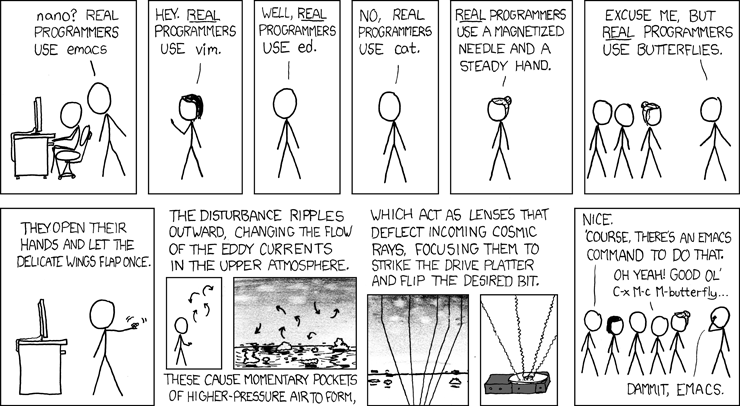
\includegraphics{emacs.png} \\
  \footnotesize\sffamily\flushleft\vspace{-\baselineskip}%
  Tiré de \href{http://xkcd.com/378/}{XKCD.com}. La commande \code{M-X
    butterfly} existe vraiment dans Emacs... en référence à cette
  bande dessinée!
\end{figure}
\setkeys{Gin}{width=0.8\textwidth}

\section{Mise en contexte}
\label{emacs+ess:contexte}

Emacs est le logiciel étendard du projet GNU («\emph{GNU is not
  Unix}»), dont le principal commanditaire est la \emph{Free Software
  Foundation} (FSF) à l'origine de tout le mouvement du logiciel
libre.
\begin{itemize}
\item Richard M.\ Stallman, président de la FSF et grand apôtre du
  libre, a écrit la première version de Emacs et il continue à ce jour
  à contribuer au projet.
\item Les origines de Emacs remontent au début des années 1980, une
  époque où les interfaces graphiques n'existaient pas, le parc
  informatique était beaucoup plus hétérogène qu'aujourd'hui (les
  claviers n'étaient pas les mêmes d'une marque d'ordinateur à une
  autre) et les modes de communication entre les ordinateurs
  demeuraient rudimentaires.
\item L'âge vénérable de Emacs transparaît à plusieurs endroits,
  notamment dans la terminologie inhabituelle, les raccourcis clavier
  non conformes aux standards d'aujourd'hui ou la manipulation des
  fenêtres qui ne se fait pas avec une souris.
\end{itemize}

Emacs s'adapte à différentes tâches par l'entremise de \emph{modes}
qui modifient son comportement ou lui ajoutent des fonctionnalités.
L'un de ces modes est ESS (\emph{Emacs Speaks Statistics}).
\begin{itemize}
\item ESS permet d'interagir avec des logiciels statistiques (en
  particulier R, S+ et SAS) directement depuis Emacs.
\item Quelques-uns des développeurs de ESS sont aussi des développeurs
  de R, d'où la grande compatibilité entre les deux logiciels.
\item Lorsque ESS est installé, le mode est activé automatiquement en
  ouvrant dans Emacs un fichier dont le nom se termine par l'extension
  \code{.R}.
\end{itemize}


\section{Installation}
\label{emacs+ess:installation}

GNU Emacs et le mode ESS sont normalement livrés d'office avec toutes
les distributions Linux. Pour les environnements Windows et OS~X,
le plus simple consiste à installer les distributions préparées par le
présent auteur. Consulter le site
\begin{quote}
  \url{http://vgoulet.act.ulaval.ca/emacs/}
\end{quote}


\section{Description sommaire}
\label{emacs+ess:description}

Au lancement, Emacs affiche un écran d'information contenant des liens
vers différentes ressources. Cet écran disparaît dès que l'on appuie
sur une touche. La fenêtre Emacs se divise en quatre zone principales
(voir la \autoref{fig:ess:emacswindow}):
\begin{enumerate}
\item tout au haut de la fenêtre (ou de l'écran sous OS~X), on trouve
  l'habituelle barre de menu dont le contenu change selon le mode dans
  lequel se trouve Emacs;
\item l'essentiel de la fenêtre sert à afficher un \emph{buffer}, soit
  le contenu d'un fichier ouvert ou l'invite de commande d'un
  programme externe;
\item la ligne de mode est le séparateur horizontal contenant diverses
  informations sur le fichier ouvert et l'état de Emacs;
\item le \emph{minibuffer} est la région au bas de la fenêtre où l'on
  entre des commandes et reçoit de l'information de Emacs.
\end{enumerate}
Il est possible de séparer la fenêtre Emacs en sous-fenêtres pour
afficher plusieurs \emph{buffers} à la fois. Il y a alors une ligne de
mode pour chaque \emph{buffer}.

\begin{figure}[t]
  %% Capture d'écran
  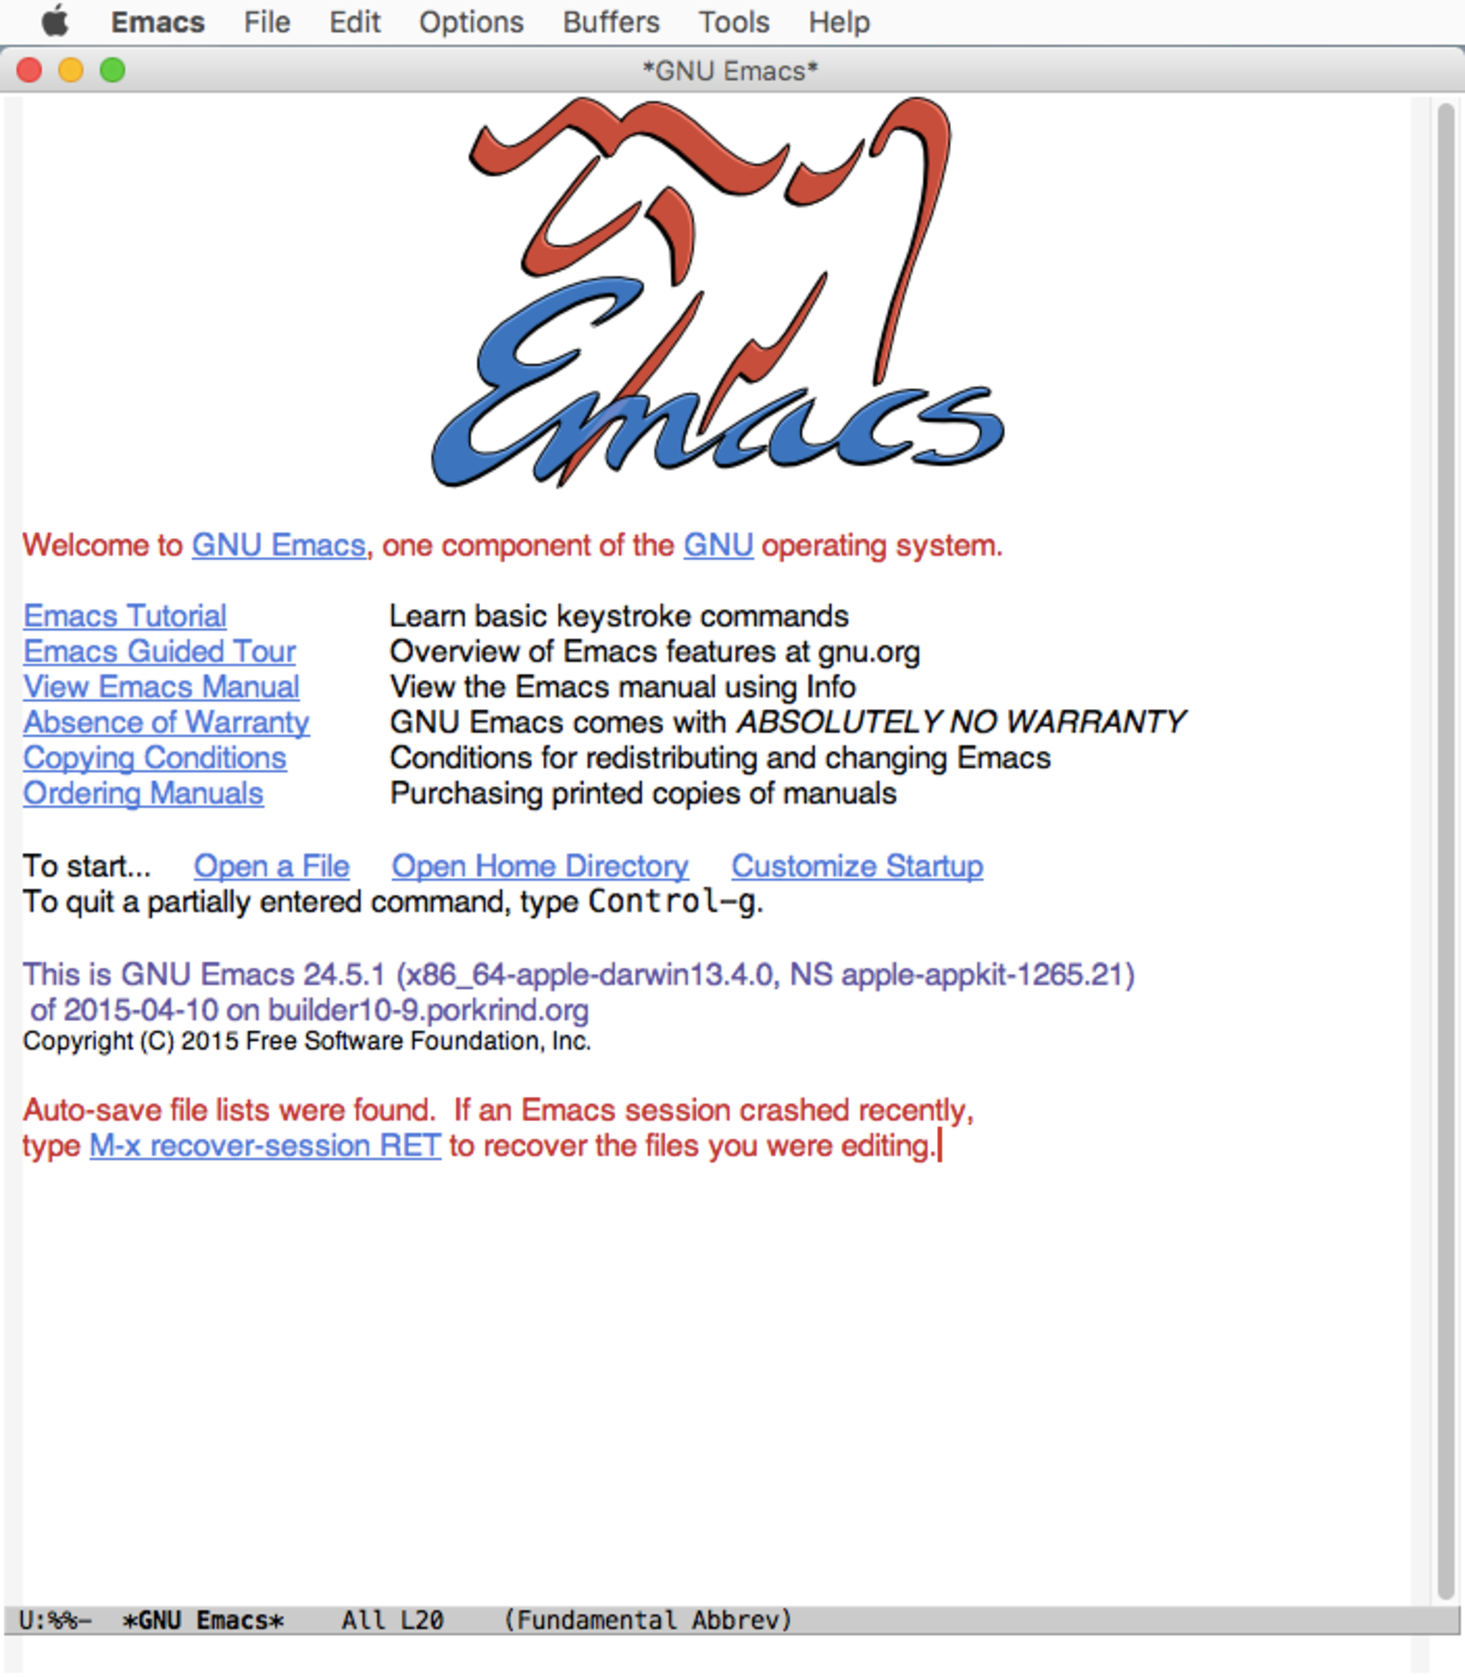
\includegraphics{emacswindow-screenshot}

  %% Identification de la barre de menu
  \begin{textblock}{0.35}(7.38,-6.58)
    \Large\faLongArrowRight
  \end{textblock}
  \begin{textblock}{1.75}(7.88,-6.59)
    \footnotesize\sffamily Barre de menu
  \end{textblock}

  %% Identification du buffer
  \begin{textblock}{0.35}(7.38,-3.38)
    \Large\faLongArrowRight
  \end{textblock}
  \begin{textblock}{1.75}(7.88,-3.39)
    \footnotesize\sffamily \emph{Buffer}
  \end{textblock}

  %% Identification de la mode line
  \begin{textblock}{0.35}(7.38,-0.28)
    \Large\faLongArrowRight
  \end{textblock}
  \begin{textblock}{1.75}(7.88,-0.29)
    \footnotesize\sffamily Ligne de mode
  \end{textblock}

  %% Identification du minibuffer
  \begin{textblock}{0.35}(7.38,-0.08)
    \Large\faLongArrowRight
  \end{textblock}
  \begin{textblock}{1.75}(7.88,-0.09)
    \footnotesize\sffamily \emph{Minibuffer}
  \end{textblock}
  \caption{Fenêtre GNU~Emacs et ses différentes parties au lancement
    de l'application sous OS~X. Sous Windows et Linux, la barre de
    menu se trouve à l'intérieur de la fenêtre.}
  \label{fig:ess:emacswindow}
\end{figure}


\section{\emph{Emacs-ismes} et \emph{Unix-ismes}}
\label{emacs+ess:ismes}

Emacs possède sa propre terminologie qu'il vaut mieux connaître
lorsque l'on consulte la documentation. De plus, l'éditeur utilise des
conventions du monde Unix qui sont moins usitées sur les plateformes
Windows et OS~X.

\begin{itemize}
\item Dans les définitions de raccourcis claviers:
  \begin{itemize}
  \item \code{C} est la touche \code{Contrôle} (\ctlkey);
  \item \code{M} est la touche \code{Meta}, qui correspond à la touche
    \code{Alt} de gauche sur un PC ou la touche \code{Option}
    (\optkey) sur un Mac (toutefois, voir l'encadré à la
    \autopageref{fig:ess:meta});
  \item \code{ESC} est la touche \code{Échap} (\esckey) et
    est équivalente à \code{Meta};
  \item \code{SPC} est la barre d'espacement;
  \item \code{DEL} est la touche \code{Retour arrière} (\delkey) ---
    \emph{et non la touche} \code{Supprimer}.
  \item \code{RET} est la touche \code{Entrée} (\returnkey);
  \end{itemize}
\item Toutes les fonctionnalités de Emacs correspondent à une commande
  pouvant être tapée dans le \emph{minibuffer}. \code{M-x} démarre
  l'invite de commande.
\item Le caractère \,\verb=~=\, représente le dossier vers lequel
  pointe la variable d'environnement \code{\$HOME} (Linux, OS~X) ou
  \code{\%HOME\%} (Windows). C'est le dossier par défaut de Emacs.
\item La barre oblique (\code{/}) est utilisée pour séparer les
  dossiers dans les chemins d'accès aux fichiers, même sous Windows.
\item En général, il est possible d'appuyer sur \code{TAB} dans le
  \emph{minibuffer} pour compléter les noms de fichiers ou de
  commandes.
\end{itemize}

\begin{figure}[t]
  \begin{osx}
    Par défaut sous OS~X, la touche \code{Meta} est assignée à
    \code{Option} (\optkey). Sur les claviers français, cela empêche
    d'accéder à certains caractères spéciaux tels que [, ], \{ ou \}.

    Une solution à cette fâcheuse situation consiste à assigner
    la touche \code{Meta} à \code{Commande} (\cmdkey). Cela bloque
    alors l'accès à certains raccourcis Mac, mais la situation est
    moins critique ainsi.

    Pour assigner la touche \code{Meta} à \code{Commande} (\cmdkey) et
    laisser la touche \code{Option} (\optkey) jouer son rôle usuel, il
    suffit d'insérer les lignes suivantes dans son fichier de
    configuration \code{.emacs} (voir la
    \autoref{emacs+ess:configuration}):
\begin{verbatim}
;;; ====================================
;;;  Assigner la touche Meta à Commande
;;;  et laisser Option être Option
;;; ====================================
(setq-default ns-command-modifier 'meta)
(setq-default ns-option-modifier 'none)
\end{verbatim}
  \end{osx}
  \label{fig:ess:meta}
\end{figure}



\section{Commandes de base}
\label{emacs+ess:commandes}

Emacs comporte une pléthore de commandes, il serait donc futile de
tenter d'en faire une liste exhaustive ici. Nous nous contenterons de
mentionner les commandes les plus importantes regroupées par tâche.

% Pour débuter, il est utile de suivre le Tour guidé de Emacs\footnote{%
%   \url{http://www.gnu.org/software/emacs/tour/} ou cliquer sur le lien
%   dans l'écran d'accueil.} %
% et de lire le tutoriel de Emacs, que l'on démarre avec \code{C-h t}.

\subsection{Les essentielles}
\label{emacs+ess:commandes:essentielles}

\begin{ttscript}{M-x}
\item[\code{M-x}] démarrer l'invite de commande
\item[\code{C-g}] bouton de panique: annuler, quitter! Presser plus
  d'une fois au besoin.
\end{ttscript}

\subsection{Manipulation de fichiers}
\label{emacs+ess:commandes:fichiers}

Entre parenthèses, le nom de la commande Emacs correspondante. On peut
entrer cette commande dans le \emph{minibuffer} au lieu d'utiliser le
raccourci clavier.

\begin{important}
  On remarquera qu'il n'existe pas de commande «nouveau fichier» dans
  Emacs. Pour créer un nouveau fichier, il suffit d'ouvrir un fichier
  n'existant pas.\index{Emacs!nouveau fichier}
\end{important}

\begin{ttscript}{C-x C-w}
  \raggedright
\item[\code{C-x C-f}] ouvrir un fichier (\code{find-file})
\item[\code{C-x C-s}] sauvegarder
  (\code{save-buffer})\index{Emacs!sauvegarder}
\item[\code{C-x C-w}] sauvegarder sous
  (\code{write-file})\index{Emacs!sauvegarder sous}
\item[\code{C-x k}] fermer un fichier (\code{kill-buffer})
  \\[\baselineskip]
\item[\code{C-\_}] annuler (pratiquement illimité); aussi
  \code{C-x u} (\code{undo})
  \\[\baselineskip]
\item[\code{C-s}] recherche incrémentale avant
  (\code{isearch-forward})
\item[\code{C-r}] Recherche incrémentale arrière
  (\code{isearch-backward})
\item[\code{M-\%}] rechercher et remplacer
  (\code{query-replace})\index{Emacs!rechercher et remplacer}
\end{ttscript}


\subsection{Déplacements simples du curseur}
\index{Emacs!déplacement du curseur}
\label{emacs+ess:commandes:deplacement}

\begin{ttscript}{C-DEL | C-w}
  \raggedright
\item[\code{C-b} | \code{C-f}] déplacer d'un caractère vers l'arrière~|~l'avant
  (\code{backward-char} | \code{forward-char})
\item[\code{C-a} | \code{C-e}] aller au début~|~fin de la ligne
  (\code{move-beginning-of-line} | \code{move-end-of-line})
\item[\code{C-p} | \code{C-n}] aller à la ligne précédente~|~suivante
  (\code{previous-line} | \code{next-line})
\item[\code{M-<} | \code{M->}] aller au début~|~fin du fichier
  (\code{beginning-of-buffer} | \code{end-of-buffer}) \\[\baselineskip]
\item[\code{DEL} | \code{C-d}] effacer le caractère à
  gauche~|~droite du curseur (\code{delete-backward-char} | \code{delete-char})
\item[\code{M-DEL} | \code{M-d}] effacer le mot à gauche~|~droite
  du curseur (\code{backward-kill-word} | \code{kill-word})
\item[\code{C-k}] supprimer jusqu'à la fin de la ligne (\code{kill-line})
\end{ttscript}

\begin{figure}[ht]
  \begin{osx}
    Plusieurs des raccourcis clavier de Emacs composés avec la touche
    \code{Contrôle} (\ctlkey) sont valides sous OS~X. Par exemple,
    \ctlkey\,\code{A} et \ctlkey\,\code{E} déplacent le curseur au
    début et à la fin de la ligne dans les champs texte.
  \end{osx}
\end{figure}


\subsection{Sélection de texte, copier, coller, couper}
\index{Emacs!sélection}
\label{emacs+ess:commandes:selection}

\begin{ttscript}{C-x C-w}
  \raggedright
\item[\code{C-SPC}] débute la sélection (\code{set-mark-command})
\item[\code{C-w}] couper la sélection (\code{kill-region})
\item[\code{M-w}] copier la sélection (\code{kill-ring-save})
\item[\code{C-y}] coller (\code{yank})
\item[\code{M-y}] remplacer le dernier texte collé par la
  sélection précédente (\code{yank-pop})
\end{ttscript}

\begin{itemize}
\item Il est possible d'utiliser les raccourcis clavier usuels de
  Windows (\code{C-c}, \code{C-x}, \code{C-v}) et OS~X
  (\cmdkey\,\code{C}, \cmdkey\,\code{X}, \cmdkey\,\code{V}) en
  activant le mode CUA dans le menu \code{Options}.
\item On peut copier-coller directement avec la souris dans Windows en
  sélectionnant du texte puis en appuyant sur le bouton central (ou la
  molette) à l'endroit souhaité pour y copier le texte.
\end{itemize}


\subsection{Manipulation de fenêtres}
\label{emacs+ess:commandes:fenetres}

\begin{ttscript}{C-x C-w}
\item[\code{C-x b}] changer de \emph{buffer}
  (\code{switch-buffer})
\item[\code{C-x 2}] séparer l'écran en deux fenêtres
  (\code{split-window-vertically})
\item[\code{C-x 1}] conserver uniquement la fenêtre courante
  (\code{delete-other-windows})
\item[\code{C-x 0}] fermer la fenêtre courante
  (\code{delete-window})
\item[\code{C-x o}] aller vers une autre fenêtre lorsqu'il y en a
  plus d'une (\code{other-window})
\end{ttscript}

\subsection{Manipulation de fichiers de script dans le mode ESS}
\index{Emacs!mode ESS|(}
\label{emacs+ess:commandes:script}

Le mode ESS dispose de fonctions «intelligentes» qui facilitent
grandement la manipulation des fichiers de script. Les deux
principales commandes à connaître sont les suivantes:
\begin{ttscript}{C-x C-w}
  \raggedright
\item[\code{C-RET}] évaluer dans le processus R la ligne sous le
  curseur ou la région sélectionnée, puis déplacer le curseur à la
  prochaine expression (\code{ess-eval-region-or-line-and-step})
\item[\code{C-c C-c}] évaluer dans le processus R la région
  sélectionnée, la fonction ou le paragraphe (tout bloc entre deux
  lignes blanches) dans lequel se trouve le curseur, puis déplacer le
  curseur à la prochaine expression
  (\code{ess-eval-region-or-function-or-paragraph-and-step})
\end{ttscript}
Les quelques autres fonctions utiles sont:
\begin{ttscript}{C-x C-w}
  \raggedright
\item[\code{C-c C-z}] déplacer le curseur vers le processus R
  (\code{ess-switch-to-inferior-or-script-buffer})
\item[\code{C-c C-f}] évaluer le code de la fonction courante dans
  le processus R (\code{ess-eval-function})
\item[\code{C-c C-l}] évaluer le code du fichier courant en entier dans
  le processus R (\code{ess-load-file})
\item[\code{C-c C-v}] aide sur une commande R
  (\code{ess-display-help-on-object})
\end{ttscript}

\subsection{Interaction avec l'invite de commande R}
\label{emacs+ess:commandes:invite}

\begin{ttscript}{M-p |M-n}
  \raggedright
\item[\code{M-p} | \code{M-n}] commande précédente~|~suivante
  dans l'historique (\code{previous-matching-history-from-input},
  \code{next-matching-history-from-input})
\item[\code{C-c C-z}] déplacer le curseur vers le fichier de script
  courant (\code{ess-switch-to-inferior-or-script-buffer})
\item[\code{M-h}] sélectionner le résultat de la dernière commande
  (\code{mark-paragraph})
\item[\code{C-c C-o}] effacer le résultat de la dernière commande
  (\code{comint-delete-output})
\item[\code{C-c C-v}] aide sur une commande R
  (\code{ess-display-help-on-object})
\item[\code{C-c C-q}] terminer le processus R (\code{ess-quit})
\end{ttscript}

\subsection{Consultation des rubriques d'aide de R}
\label{emacs+ess:commandes:aide}

\begin{ttscript}{m, m}
  \raggedright
\item[\code{p} | \code{n}] aller à la section précédente~|~suivante de
  la rubrique (\code{ess-skip-to-previous-section} |
  \code{ess-skip-to-next-section})
\item[\code{s a}] aller à la section de la liste des arguments \emph{(Arguments)}
\item[\code{s D}] aller à la section des détails sur la fonction \emph{(Details)}
\item[\code{s v}] aller à la section sur la valeur retournée par la
  fonction \emph{(Value)}
\item[\code{s s}] aller à la section des fonctions apparentée \emph{(See Also)}
\item[\code{s e}] aller à la section des exemples \emph{(Examples)}
\item[\code{l}] évaluer la ligne sous le curseur; pratique pour
  exécuter les exemples (\code{ess-eval-line-and-step})
\item[\code{r}] évaluer la région sélectionnée (\code{ess-eval-region})
\item[\code{h}] ouvrir une nouvelle rubrique d'aide, par défaut pour le
  mot se trouvant sous le curseur (\code{ess-display-help-on-object})
\item[\code{q}] retourner au processus ESS en laissant la rubrique
  d'aide visible (\code{ess-switch-to-end-of-ESS})
\item[\code{x}] fermer la rubrique d'aide et retourner au processus ESS
  (\code{ess-kill-buffer-and-go})
\end{ttscript}



\section{Anatomie d'une session de travail (bis)}
\label{emacs+ess:session}

On reprend ici les étapes d'une \capsule{http://youtu.be/xiNnHegDau8}{session de
  travail} type présentées à la \autoref{presentation:session}, mais
en expliquant comment compléter chacune dans Emacs avec le mode ESS.

\begin{enumerate}
\item Lancer Emacs et ouvrir un fichier de script avec
  \begin{quote}
    \code{C-x C-f}
  \end{quote}
  ou avec le menu
  \begin{quote}
    \code{File|Open File...}
  \end{quote}
  En spécifiant un nom de fichier qui n'existe pas déjà, on se trouve
  à créer un nouveau fichier de script. S'assurer de terminer le nom
  du nouveau fichier par \code{.R} pour que Emacs reconnaisse
  automatiquement qu'il s'agit d'un fichier de script R.
\item Démarrer un processus R à l'intérieur même de Emacs avec
  \begin{quote}
    \code{M-x R }\returnkey
  \end{quote}
  Emacs demandera alors de spécifier de répertoire de travail
  (\emph{starting data directory}). Accepter la valeur par défaut, par
  exemple
  \begin{quote}
    \verb=~/ =\returnkey
  \end{quote}
  ou indiquer un autre dossier. Un éventuel message de Emacs à l'effet
  que le fichier \code{.Rhistory} n'a pas été trouvé est sans
  conséquence et peut être ignoré.
\item Composer le code. Lors de cette étape, on se déplacera souvent
  du fichier de script à la ligne de commande afin d'essayer diverses
  expressions. On exécutera également des parties seulement du code se
  trouvant dans le fichier de script. Les commandes les plus utilisées
  sont alors:
  \begin{quote}
    \begin{ttscript}{C-c C-z}
      \renewcommand{\makelabel}[1]{#1\hfill}
    \item[\code{C-RET}] pour exécuter une ligne du fichier de script ou la
      région sélectionnée;
    \item[\code{C-c C-c}] pour exécuter un paragraphe du fichier de
      script;
    \item[\code{C-c C-z}] pour se déplacer entre le fichier de script et
      la ligne de commande R.
    \end{ttscript}
  \end{quote}
\item Sauvegarder le fichier de script:
  \begin{quote}
    \code{C-x C-s}
  \end{quote}
  Les quatrième et cinquième caractères de la ligne de mode changent
  de \,\verb|**|\, à \,\verb|--|.
\item Sauvegarder si désiré l'espace de travail de R avec
  \code{save.image()}\indexfonction{save.image}. Cela n'est
  habituellement pas nécessaire à moins que l'espace de travail ne
  contienne des objets importants ou longs à recréer.
\item Quitter le processus R avec
  \begin{quote}
    \code{C-c C-q}
  \end{quote}
  Cette commande ESS se chargera de fermer tous les fichiers associés
  au processus R. On peut ensuite quitter Emacs en fermant
  l'application de la manière usuelle.
\end{enumerate}
\index{Emacs!mode ESS|)}



\section{Configuration de l'éditeur}
\label{emacs+ess:configuration}

Une des grandes forces de Emacs est qu'à peu près chacune de ses
facettes est configurable: couleurs, polices de caractère, raccourcis
clavier, etc.

\begin{itemize}
\item La configuration de Emacs se fait par le biais de commandes
  réunies dans un \capsule{http://youtu.be/IsyQn7d2Ao0}{fichier de
    configuration} nommé \code{.emacs} (le point est important!) que
  Emacs lit au démarrage.
\item Le fichier \code{.emacs} doit se trouver dans le dossier
  \,\verb=~/=, c'est-à-dire dans le dossier de départ de l'utilisateur
  sous Linux et OS~X, et dans le dossier référencé par la variable
  d'environnement \code{\%HOME\%} sous Windows.
\end{itemize}


\section{Aide et documentation}
\label{emacs+ess:aide}

Emacs possède son propre système d'aide très exhaustif, mais dont la
navigation est peu intuitive selon les standards d'aujourd'hui.
Consulter le menu \code{Help}.

Autrement, on trouvera les manuels de Emacs et de ESS en divers
formats dans les sites respectifs des deux projets:
\begin{quote}
  \url{http://www.gnu.org/software/emacs} \\
  \url{http://ess.r-project.org}
\end{quote}

Enfin, si le désespoir vous prend au cours d'une séance de codage
intensive, vous pouvez toujours consulter le psychothérapeute Emacs.
On le trouve, bien entendu, dans le menu \code{Help}!

\index{Emacs|)}

%%% Local Variables:
%%% mode: latex
%%% TeX-master: "introduction_programmation_r"
%%% coding: utf-8
%%% End:

\chapter{RStudio: une introduction}
\index{RStudio|(}
\label{chap:rstudio}

Un environnement de développement intégré (\emph{integrated
  development environment}, IDE) est un progiciel de productivité
destiné au développement de logiciels ou, plus largement, à la
programmation informatique. Il comprend toujours un éditeur de texte
adapté au langage de programmation visé, un environnement de
compilation ou d'exécution du code et, généralement, des outils de
contrôle de versions, de gestion des projets et de navigation dans le
code source.\footnote{%
  À ce compte, GNU~Emacs constitue un environnement de développement
  intégré.} %

Offert au public depuis 2011, RStudio est un IDE convivial conçu
spécifiquement pour l'analyse de données et le développement de
packages avec R. Il est produit par RStudio~Inc.\ et est offert en
version libre ou commerciale, pour une exécution locale
(\emph{desktop}) ou pour une exécution sur un serveur via un
navigateur web.


\section{Installation}
\label{sec:rstudio:installation}

RStudio est disponible à l'identique pour les plateformes Windows,
macOS et Linux. Pour une utilisation locale sur son poste de travail,
on installera la version libre (\emph{Open Source}) de
\link{https://www.rstudio.com/products/rstudio/download/}{RStudio~Desktop}.


\section{Description sommaire}
\label{sec:rstudio:description}

La fenêtre de RStudio se divise toujours en quatre
sous-fenêtres\footnote{%
  Les sous-fenêtres sont appelées \emph{panes} (en anglais) dans
  l'application.} %
--- sauf au lancement, alors que la sous-fenêtre d'édition de code
source n'est pas visible; voir la \autoref{fig:rstudio:rstudiowindow}.
Dans le sens des aiguilles d'une montre en partant en haut à gauche,
on trouve:
\begin{enumerate}
  \index{RStudio!sous-fenêtres}
\item la sous-fenêtre d'édition de code source, avec un onglet par
  fichier de script;
\item le navigateur d'environnement de travail ou d'historique des
  commandes, selon l'onglet sélectionné;
\item le navigateur de fichiers du projet, de packages, de graphiques,
  etc., selon l'onglet sélectionné;
\item la console --- ou ligne de commande --- R.
\end{enumerate}
Au lancement de l'application, la console R occupe toute la gauche de
la fenêtre jusqu'à ce qu'un fichier de script soit ouvert.

\begin{figure}[t]
  %% Capture d'écran et espace additionnel sous l'image
  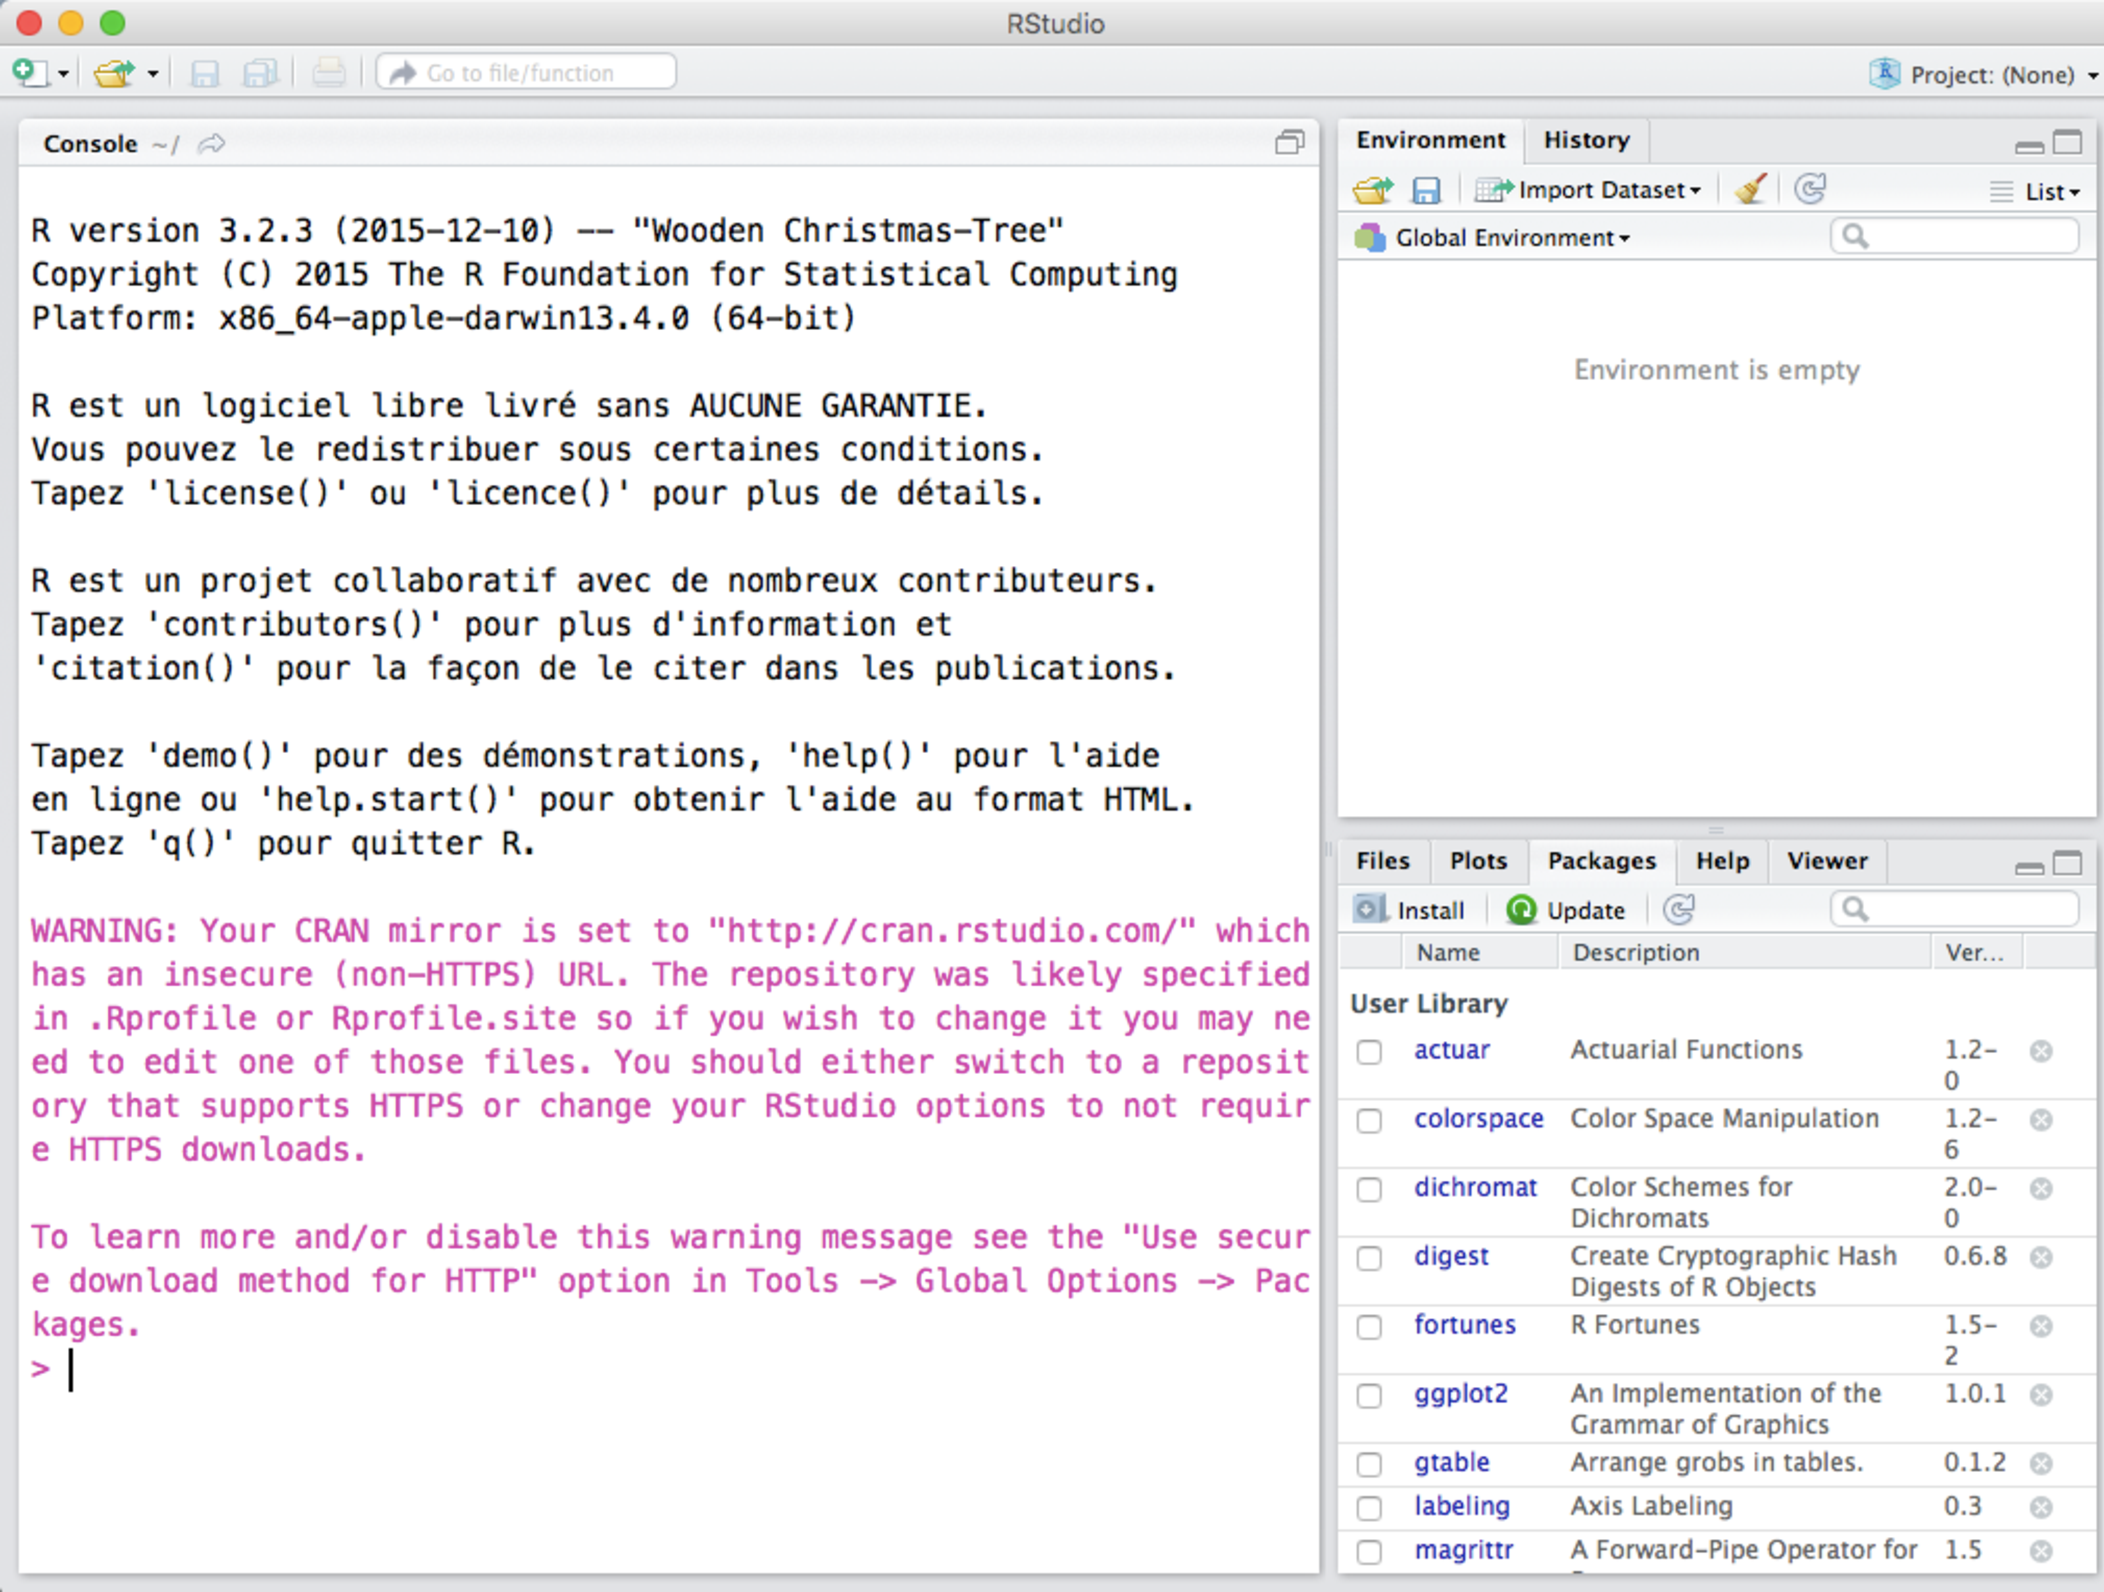
\includegraphics{rstudiowindow-screenshot}
  \vspace{0.5\TPVertModule}

  \begingroup
  \TPoptions{absolute=false}
  %% Identification de la console
  \begin{textblock}{0.5}(2.65,-0.62)
    \large\faLongArrowDown
  \end{textblock}
  \begin{textblock}{2}(2.2,-0.3)
    \footnotesize\sffamily Console R
  \end{textblock}

  %% Identification du navigateur d'environnement
  \begin{textblock}{1}(7.52,-3.65)
    \large\faLongArrowRight
  \end{textblock}
  \begin{textblock}{2.2}(7.95,-3.9)
    \footnotesize\sffamily\raggedright Navigateur d'environnement et d'historique
  \end{textblock}

  %% Identification de navigateur de fichiers
  \begin{textblock}{1}(7.52,-1.65)
    \large\faLongArrowRight
  \end{textblock}
  \begin{textblock}{2.2}(7.95,-1.9)
    \footnotesize\sffamily\raggedright Navigateur de fichiers, packages, graphiques, etc.
  \end{textblock}
  \endgroup
  \caption{Fenêtre de RStudio et trois de ses sous-fenêtres au
    lancement de l'application sous macOS. Sous Windows et Linux, la
    fenêtre comporte également une barre de menu.}
  \label{fig:rstudio:rstudiowindow}
\end{figure}

\begin{itemize}
\item Le navigateur d'environnement de travail est particulièrement
  utile pour voir le contenu, les attributs, le type et la taille de
  chaque objet sauvegardé dans la session R. Il permet également de
  visualiser le contenu des objets en cliquant sur leur nom ou sur
  l'icône de grille à droite de leur nom.
\item Il ne peut y avoir qu'un seul processus R (affiché dans la
  console) actif par fenêtre RStudio. Pour utiliser plusieurs
  processus R simultanément, il faut démarrer autant de copies de
  RStudio.
\item La position des sous-fenêtres dans la grille ne peut être
  modifiée. Par contre, chaque sous-fenêtre peut être redimensionnée.
\item On peut modifier la liste des onglets affichés dans les deux
  navigateurs dans les préférences de l'application; voir la
  \autoref{sec:rstudio:configuration}.
\end{itemize}


\section{Projets}
\index{RStudio!projets}
\label{sec:rstudio:projets}

Il est possible d'utiliser RStudio un peu comme un simple éditeur de
texte.
\begin{itemize}
\item On ouvre les fichiers de scripts un à un, soit à partir du menu
  \code{File|Open file...}, soit à partir de l'onglet \code{Files} du
  navigateur de fichiers.
\item Lorsque nécessaire, on change le répertoire de travail de R à
  partir du menu \code{Session}.
\end{itemize}

Pour faciliter l'organisation de son travail, l'ouverture des fichiers
de script et le lancement d'un processus R dans le bon répertoire de
travail, RStudio propose la notion de \emph{projet}.
\begin{itemize}
\item Un projet RStudio est associé à un répertoire de travail de R
  (\autoref{sec:presentation:workspace}).
\item On crée un nouveau projet à partir du menu \code{Project} à
  l'extrémité droite de la barre d'outils ou à partir du menu
  \code{File|New Project...} On a alors l'option de créer un nouveau
  dossier sur notre poste de travail ou de créer un projet à partir
  d'un dossier existant.
\item Lors de la création d'un projet, RStudio crée dans le dossier
  visé un fichier avec une extension \code{.Rproj} contenant diverses
  informations en lien avec le projet. De plus, le projet est
  immédiatement chargé dans RStudio.
\item L'ouverture d'un projet entraine: le lancement d'une session R
  dont le répertoire de travail est celui du projet; le
  chargement du fichier \code{.RData} (le cas échéant); l'ouverture de
  tous les fichiers de scripts qui étaient ouverts lors de la dernière
  séance de travail.
\item Chaque projet dispose de ses propres réglages. On accède à
  ceux-ci via la commande \code{Project Options...} du menu
  \code{Project} de la barre d'outils.
\end{itemize}

On trouvera plus d'information sur les projets dans l'aide en ligne
de RStudio.


\section{Commandes de base}
\label{sec:rstudio:commandes}

Comme l'interface de RStudio respecte les standards modernes, je ne
souligne ici que les commandes particulièrement utiles pour la
manipulation des fichiers de script. On accède rapidement à la liste
des commandes les plus utiles via le menu \code{Help} de
l'application.

Les raccourcis clavier sous, d'une part, Windows et Linux et sous,
d'autre part, macOS, différent légèrement. Je fournis ci-dessous
les deux jeux, séparés par le symbole $\bullet$.

\begin{ttscript}{Ctrl-Shift-S $\bullet$ \cmdkey\shiftkey S}
  \index{RStudio!symbole d'affectation}
\item[\code{Alt+-} $\bullet$ \code{\optkey\,-}] insérer le symbole
  d'affectation \verb*| <- | (pour les
  \capsule{https://youtu.be/aTyJfzE6pRw}{Mac avec un clavier
    canadien-français}, consulter l'encadré de la
  \autopageref{fig:rstudio:affectation})
\item[\code{Ctrl+Retour} $\bullet$ \code{\cmdkey\,\returnkey}]
  évaluer dans le processus R la ligne sous le curseur ou la région
  sélectionnée, puis déplacer le curseur à la prochaine expression
\item[\code{Ctrl+Shift+S} $\bullet$ \code{\shiftkey\,\cmdkey\,S}]
  évaluer le code du fichier courant en entier dans le processus R
\item[\code{Ctrl+Alt+B} $\bullet$ \code{\optkey\,\cmdkey\,B}]
  évaluer dans le processus R le code source du début du fichier
  jusqu'à la ligne sous le curseur
\item[\code{Ctrl+Alt+E} $\bullet$ \code{\optkey\,\cmdkey\,E}]
  évaluer dans le processus R le code source de la ligne sous le curseur
  jusqu'à la fin du fichier
\item[\code{Ctrl+Alt+F} $\bullet$ \code{\optkey\,\cmdkey\,F}]
  évaluer le code de la fonction courante dans le processus R
\end{ttscript}

À la console --- ou ligne de commande --- R, les raccourcis suivants
sont particulièrement utiles.
\begin{ttscript}{Ctrl-I $\bullet$ \cmdkey\,I}
\item[$\uparrow$ | $\downarrow$] expression
  précédente~|~suivante dans l'historique des commandes
\item[\code{Ctrl+}$\uparrow$ $\bullet$ \cmdkey\,$\uparrow$] afficher
  la fenêtre d'historique des commandes
\end{ttscript}

\begin{figure}[t]
  \begin{emphbox}{\mdseries Symbole d'affectation et
      Mac munis d'un clavier canadien-français}
    Le très pratique raccourci clavier {\optkey\,-} servant à insérer
    le symbole d'affectation ne fonctionne pas avec le clavier
    canadien-français sur les Mac. Cette combinaison de touches sert
    déjà à insérer le symbole \textbar. C'est en fait un doublon
    puisque, si l'on en croit le clavier, ce symbole est
    principalement lié à la
    touche {\optkey\,/}.

    Il est possible de régler le problème en redéfinissant le raccourci
    clavier associé au symbole d'affectation.

    \begin{enumerate}
    \item Ouvrir les préférences de RStudio (menu
      \code{RStudio|Preferences} ou {\cmdkey\,,}).
    \item Choisir la section \code{Code} dans la barre latérale de la
      fenêtre des options.
    \item Appuyer sur le bouton \code{Modify Keyboard Shortcuts\dots}.
    \item Une nouvelle fenêtre liste toutes les commandes disponibles
      et les raccourcis clavier associés. Dans le champ de recherche en
      haut, taper les lettres de «assignment» jusqu'à ce que la
      commande \code{Insert Assignment Operator} apparaisse.
    \item Cliquer sur la case du raccouci clavier (qui devrait être
      \code{Alt+-} par défaut) pour l'activer. Appuyer sur \optkey\,-
      pour utiliser cette combinaison de touches comme raccourci. Oui,
      on entre ce qui est apparemment la même combinaison de touches.
      Pour une raison quelconque, c'est «Alt+\bs» qui apparait alors
      comme raccourci.
    \item Fermer toutes les fenêtres de configuration.
    \end{enumerate}
  \end{emphbox}
  \label{fig:rstudio:affectation}
\end{figure}

\section{Anatomie d'une session de travail (bis)}
\label{sec:rstudio:session}

On reprend ici la description de %
%\capsule{http://youtu.be/xiNnHegDau8}{session de travail} %
la session de travail %
type présentée à la \autoref{sec:presentation:session}, mais en
expliquant comment compléter chaque étape dans RStudio. Sont
intercalés dans les instructions les raccourcis clavier des commandes
RStudio et les accès par les menus.

\begin{enumerate}
\item Lancer RStudio et ouvrir un nouveau fichier de script ou un
  fichier de script existant.
  \begin{trivlist}
  \item
    \makebox[0.38\linewidth][l]{%
      \colorbox{codebg}{\code{Ctrl+Shift+N} $\bullet$ \code{\shiftkey\,\cmdkey\,N}}}
    \hfill
    \makebox[0.58\linewidth][l]{%
      \colorbox{codebg}{\code{File|New File|R Script...}}}
  \item
    \makebox[0.38\linewidth][l]{%
      \colorbox{codebg}{\code{Ctrl+O} $\bullet$ \code{\cmdkey\,O}}}
    \hfill
    \makebox[0.58\linewidth][l]{%
      \colorbox{codebg}{\code{File|Open File...}}}
  \end{trivlist}
\item C'est une bonne pratique de faire du dossier où se trouve son ou
  ses fichiers de scripts le répertoire de travail de R.
  \begin{trivlist}
  \item
    \colorbox{codebg}{\code{Session|Set Working Directory|To Source File Location}}
  \end{trivlist}
\item Composer le code. Lors de cette étape de programmation, on se
  déplacera souvent du fichier de script à la console R afin
  d'essayer diverses expressions. On exécutera également des parties
  seulement du code se trouvant dans le fichier de script.
  \begin{trivlist}
  \item
    \makebox[0.38\linewidth][l]{%
      \colorbox{codebg}{\code{Ctrl+Retour} $\bullet$ \code{\cmdkey\,\returnkey}}}
    \hfill
    \makebox[0.58\linewidth][l]{%
      \colorbox{codebg}{\code{Code|Run Selected Line(s)}}}
  \item
    \makebox[0.38\linewidth][l]{%
      \colorbox{codebg}{\code{Ctrl+1} $\bullet$ \code{\cmdkey\,1}}}
    \hfill
    \makebox[0.58\linewidth][l]{%
      \colorbox{codebg}{\code{View|Move Focus to Source}}}
  \item
    \makebox[0.38\linewidth][l]{%
      \colorbox{codebg}{\code{Ctrl+2} $\bullet$ \code{\cmdkey\,2}}}
    \hfill
    \makebox[0.58\linewidth][l]{%
      \colorbox{codebg}{\code{View|Move Focus to Console}}}
  \end{trivlist}
\item Sauvegarder le fichier de script.
  \begin{trivlist}
  \item
    \makebox[0.38\linewidth][l]{%
      \colorbox{codebg}{\code{Ctrl+S} $\bullet$ \code{\cmdkey\,S}}}
    \hfill
    \makebox[0.58\linewidth][l]{%
      \colorbox{codebg}{\code{File|Save}}}
  \end{trivlist}
  (S'il s'agit d'un nouveau fichier, s'assurer de terminer son nom par
  \code{.R}.) Le nom du fichier dans l'onglet de la sous-fenêtre passe
  du rouge au noir.
\item Sauvegarder, si désiré, l'espace de travail de R avec
  \code{save.image()}\index{save.image@\code{save.image}}. Cela n'est
  habituellement pas nécessaire à moins que l'espace de travail ne
  contienne des objets importants ou longs à recréer.
  \begin{trivlist}
  \item
    \colorbox{codebg}{\code{Session|Save Workspace As...}}
  \end{trivlist}
\item Quitter RStudio de la manière usuelle. Par défaut, RStudio
  devrait demander si l'on souhaite sauvegarder l'espace de travail de
  R. Nous suggérons de ne pas le faire.

  La \autoref{sec:rstudio:configuration} explique comment configurer
  RStudio afin d'éviter de se faire poser la question à chaque
  fermeture de l'application.
\end{enumerate}


\section{Configuration de l'éditeur}
\index{RStudio!configuration}
\label{sec:rstudio:configuration}

Il est possible de configurer plusieurs facettes de RStudio à partir
d'une interface familière. On accède aux options de configuration par
le menu \code{Tools|Global Options...} sous Windows et Linux, et par le
menu standard \code{RStudio|Preferences} (\code{\cmdkey\,,})
sous macOS.

Nous recommandons de régler l'option
\begin{quote}
  \code{Save workspace to .RData on exit}
\end{quote}
à \code{Never} dans les options de configuration générales,
tel qu'illustré à la \autoref{fig:rstudio:rstudiopreferences}. Avec ce
réglage, l'espace de travail de R ne sera pas sauvegardé à la
fermeture de RStudio.

\begin{figure}
  \centering
  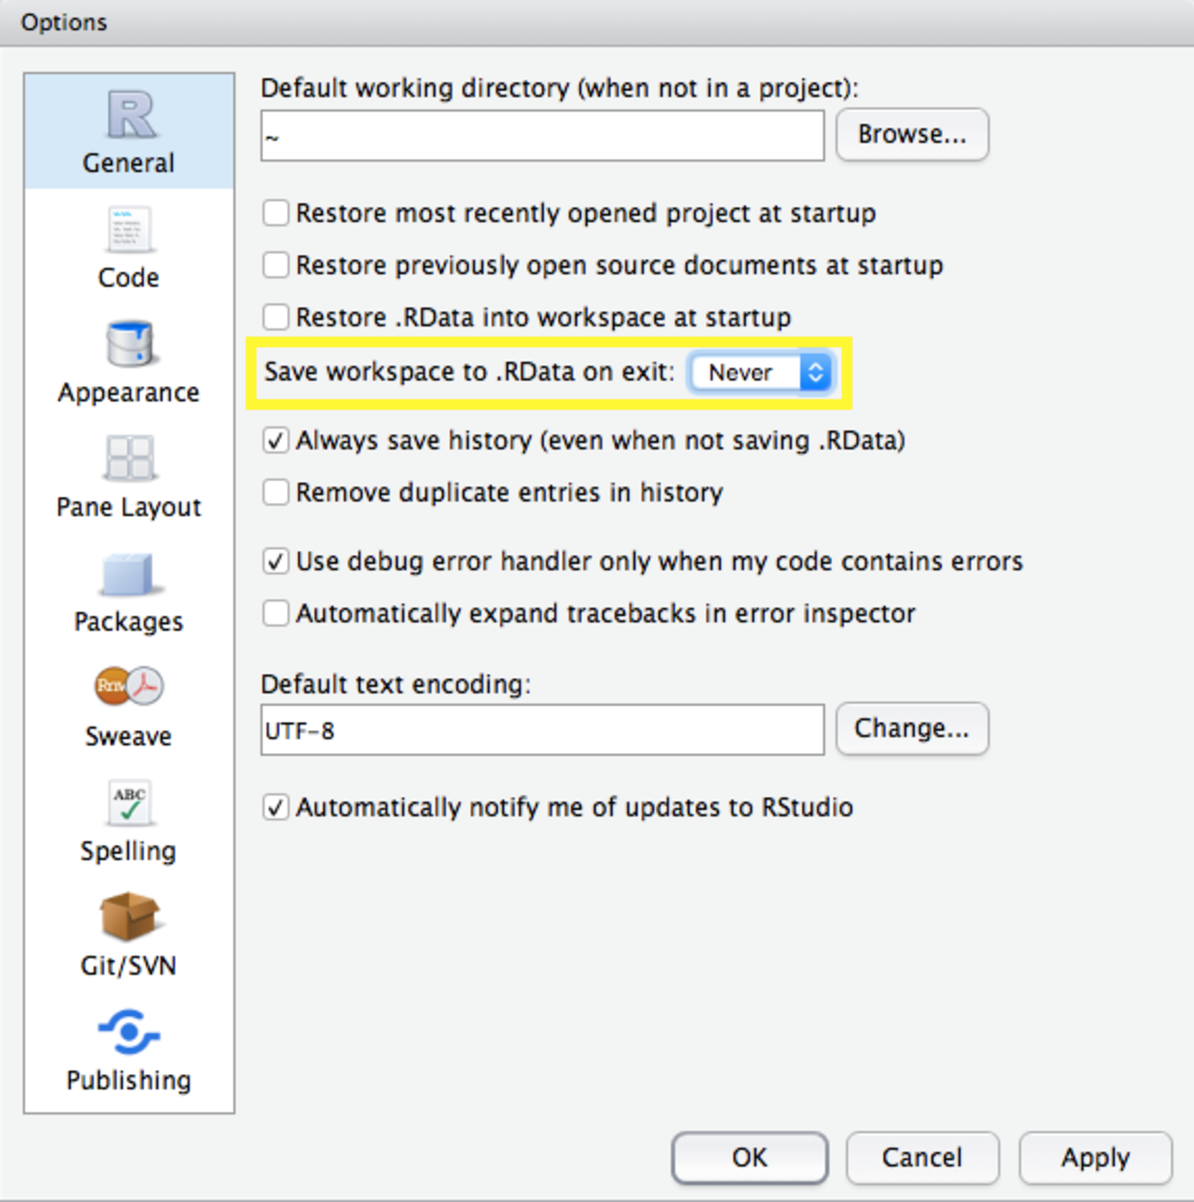
\includegraphics{rstudiopreferences-screenshot}
  \caption{Réglage suggéré de RStudio (encadré en jaune) faisant en
    sorte que l'espace de travail de R n'est jamais sauvegardé au
    moment de quitter l'application}
  \label{fig:rstudio:rstudiopreferences}
\end{figure}


\section{Aide et documentation}
\label{sec:rstudio:aide}

La documentation de RStudio se trouve entièrement en ligne. On y
accède par le menu \code{Help}. L'onglet \code{Help} du navigateur de
fichiers (sous-fenêtre en bas à droite) offre également une interface
unifiée pour accéder à l'aide de R et à celle de RStudio.

\index{RStudio|)}

%%% Local Variables:
%%% mode: latex
%%% TeX-engine: xetex
%%% TeX-master: "programmer-avec-r"
%%% coding: utf-8
%%% End:

% \chapter{Installation de packages dans R}
\index{package!installation|(}
\label{packages}

Un package R est un ensemble cohérent de fonctions, de jeux de données
et de documentation permettant de compléter les fonctionnalités du
système de base ou d'en ajouter de nouvelles. Les packages sont normalement
installés depuis le site \emph{Comprehensive R Archive Network} (CRAN;
\url{http://cran.r-project.org}).

Cette annexe explique comment configurer R pour faciliter l'%
\capsule{https://youtu.be/DL48oi2RKjM}{installation et l'administration
  de packages} %
externes.

Les instructions ci-dessous se basent sur la création d'une
bibliothèque personnelle\index{package!bibliothèque personnelle} où
seront installés les packages R téléchargés de CRAN. Il est fortement
recommandé de créer une telle bibliothèque. Cela permet d'éviter les
éventuels problèmes d'accès en écriture dans la bibliothèque
principale et de conserver les packages intacts lors des mises à jour
de R. On montre également comment spécifier le site miroir de CRAN
pour éviter d'avoir à le répéter à chaque installation de package.
\begin{enumerate}
\item Identifier le dossier de départ de l'utilisateur. En cas
  d'incertitude, examiner la valeur de la variable d'environnement
  \code{HOME}\footnote{%
    Pour les utilisateurs de GNU~Emacs sous Windows, la variable est
    créée par l'assistant d'installation de Emacs lorsqu'elle n'existe
    pas déjà.}, %
  depuis R avec la commande
\begin{Schunk}
\begin{Sinput}
> Sys.getenv("HOME")
\end{Sinput}
\end{Schunk}
  ou, pour les utilisateurs de Emacs, directement depuis l'éditeur avec
\begin{verbatim}
M-x getenv RET HOME RET
\end{verbatim}
  Nous référerons à ce dossier par le symbole \verb=~=.
\item Créer un dossier qui servira de bibliothèque de packages
  personnelle. Dans la suite, nous utiliserons \verb=~/R/library=.
\item La configuration de R se fait à l'aide simples fichiers texte,
  comme pour GNU~Emacs; voir la \autoref{emacs+ess:configuration}.
  Dans un fichier nommé \verb=~/.Renviron= (donc situé dans le dossier
  de départ), enregistrer la ligne suivante:
\begin{verbatim}
R_LIBS_USER="~/R/library"
\end{verbatim}
  Au besoin, remplacer le chemin \verb=~/R/library= par celui du
  dossier créé à l'étape précédente. Utiliser la barre oblique avant
  (\code{/}) dans le chemin pour séparer les dossiers.
  \begin{osx}
    Sous OS~X, ajouter dans le fichier \verb=~/.Renviron= la ligne
    suivante:
\begin{verbatim}
R_INTERACTIVE_DEVICE=quartz
\end{verbatim}
    Ainsi, R utilisera toujours l'interface Quartz\index{Quartz} native
    de OS~X pour afficher les graphiques.
  \end{osx}
\item Dans un fichier nommé \verb=~/.Rprofile=, enregistrer l'option
  suivante:
\begin{verbatim}
options(repos = "http://cran.ca.r-project.org")
\end{verbatim}
  Si désiré, remplacer la valeur de l'option \code{repos} par l'URL
  d'un autre site miroir de CRAN.

  Les utilisateurs de GNU~Emacs voudront ajouter une option pour
  éviter que R ait recours aux menus graphiques Tcl/Tk. Le code à
  entrer dans le fichier \verb=~/.Rprofile= sera plutôt
\begin{verbatim}
options(repos = "http://cran.ca.r-project.org",
        menu.graphics = FALSE)
\end{verbatim}
\end{enumerate}
Consulter la rubriques d'aide de \code{Startup} pour les détails sur
la syntaxe et l'emplacement des fichiers de configuration, celles de
\code{library} et \code{.libPaths} pour la gestion des bibliothèques
et celle de \code{options} pour les différentes options reconnues par
R.

Après un redémarrage de R, la bibliothèque personnelle aura préséance
sur la bibliothèque principale et il ne sera plus nécessaire de
préciser le site miroir de CRAN lors de l'installation de packages.
Ainsi, la simple commande
\begin{Schunk}
\begin{Sinput}
> install.packages("actuar")
\end{Sinput}
\end{Schunk}
téléchargera le package de fonctions actuarielles \textbf{actuar}
depuis le miroir canadien de CRAN et l'installera dans le dossier
\verb=~/R/library=. Pour charger le package en mémoire, on fera
\begin{Schunk}
\begin{Sinput}
> library("actuar")
\end{Sinput}
\end{Schunk}

On peut arriver au même résultat sans utiliser les fichiers de
configuration \code{.Renviron} et \code{.Rprofile}. Il faut cependant
recourir aux arguments \code{lib} et \code{repos} de la fonction
\code{install.packages} et à l'argument \code{lib.loc} de la fonction
\code{library}. Consulter les rubriques d'aide de ces deux fonctions
pour de plus amples informations.

\index{package!installation|)}

%%% Local Variables:
%%% mode: latex
%%% TeX-master: "introduction_programmation_r"
%%% coding: utf-8
%%% End:

\chapter{Réponses des exercices}
\label{chap:reponses}

\begingroup

%% Environnement Schunk simplifié pour l'affichage des réponses
\renewenvironment{Schunk}{%
  \setlength{\topsep}{0pt}
  \colorlet{shadecolor}{codebg}
  \begin{snugshade*}}%
  {\end{snugshade*}}

\input{solutions-informatique}
\input{solutions-bases}
\input{solutions-implementation}
\input{solutions-donnees}
\input{solutions-application}
\input{solutions-internes}

\endgroup

%%% Local Variables:
%%% mode: latex
%%% TeX-engine: xetex
%%% TeX-master: "programmer-avec-r"
%%% coding: utf-8
%%% End:


\bibliography{r,stat,informatique,vg}

\cleardoublepage
\printindex

\pagestyle{empty}

\cleartoverso
\vspace*{\fill}

\begingroup
\calccentering{\unitlength}
\begin{adjustwidth*}{\unitlength}{-\unitlength}
  \begin{flushleft}
    \small %
    Ce document a été produit avec le système de mise en page
    {\XeLaTeX}. Le texte principal est en Lucida Bright~OT 11~points,
    les mathématiques en Lucida Bright Math~OT, le code informatique
    en Lucida Grande Mono~DK et les titres en Adobe Myriad~Pro. Des
    icônes proviennent de la police Font~Awesome. Les graphiques ont
    été réalisés avec R.
  \end{flushleft}
\end{adjustwidth*}
\endgroup
\vfill


\cleartoverso
\begingroup

\TPGrid{3}{36}
\textblockorigin{0mm}{0mm}
\setlength{\parindent}{0mm}
\setlength{\banderougewidth}{2\TPHorizModule}
\setlength{\bandeorwidth}{\TPHorizModule}
\setlength{\gapwidth}{2pt}
\addtolength{\bandeorwidth}{-\gapwidth}

%% bandeau identitaire arrière
\begin{textblock*}{8.5in}[0,1](0mm,30\TPVertModule)
  \textcolor{or}{\rule{\bandeorwidth}{\TPVertModule}}%      % bande or
  \rule{\gapwidth}{0pt}%                                    % filet
  \textcolor{rouge}{\rule{\banderougewidth}{\TPVertModule}} % bande rouge
\end{textblock*}

% code-barre
\begin{textblock*}{0.9\TPHorizModule}(0.1\TPHorizModule,25\TPVertModule)
  % \includegraphics[height=4\TPVertModule]{codebarre_\ISBN}
\end{textblock*}

\endgroup

%%% Local Variables:
%%% mode: latex
%%% TeX-master: "programmer-avec-r"
%%% TeX-engine: xetex
%%% End:


\end{document}

%%% Local Variables:
%%% mode: latex
%%% TeX-engine: xetex
%%% TeX-master: t
%%% coding: utf-8
%%% End:
